

\subsection{P0 with mutation burden} \label{s:p0}

 
The Jack Birch's Unit holds a large dataset of bladder tissue samples both cancerous and non-cancerous. There are three different types of 'normal'  (or healthy or non-cancerous) bladder samples: P0 (23), Abs/Ca-differentiated (49) and undifferentiated (15). The P0 are in-situ tissues taken from healthy individual unaltered in the lab, the ABS/Ca differentiated are in-vitro which have been differentiated by the ABS/Ca protocol and lastly the undifferentiated are in-vitro samples which yet are not specialised. From the previous classifications \citet{Robertson2017-mg, Kamoun2020-tj} it is known that there are 2 major subgroups Luminal Papillary (LumP) and Basal Squamous (Ba/Sq). The former is known to share aspects with the differentiated tissue while the latter with the undifferentiated. 

In this section we used only the P0 dataset to construct a healthy network representing the co-expressed genes network in an unaltered bladder tissue. The network is built based on the pipeline described in Figure \ref{fig:N_I:network_pipeline} where instead of the tumour's gene expression the data from P0 is used, but the mutation burden for the modifiers is still used. This means that the Module Connectivity (ModCon) selects the genes which are most representative of the communities in the healthy network. These selected genes are used to compute the Module Evaluation Value score using the gene expression from TCGA. Therefore, this approach can be thought as a method to select the genes most representative for the P0 samples and how their expression changes in the tumour dataset. 

It is worth noting that there are only 23 P0 samples and this may not offer enough statistical power to find communities with specific biological functions. In addition, the Basal may be under-represented by the lack of undifferentiated tissue samples. Nevertheless, using unprocessed tissue samples may unravel new biology.

The top 4K most-relative varied genes (median/std) from P0 are used to construct the network, the same weight modifiers (Reward and Penalised see Fig \ref{fig:N_I:modifiers}) are employed and 50 edges for the Transcription Factor. For the standard genes 3 edges are kept while for Transcription Factors (TFs) 50. The top 100 genes are selected with ModCon and for MEVs the top 4K most varied genes are used.


\subsubsection{Describing the Network}


\begin{figure}[!htb]    
    \centering
    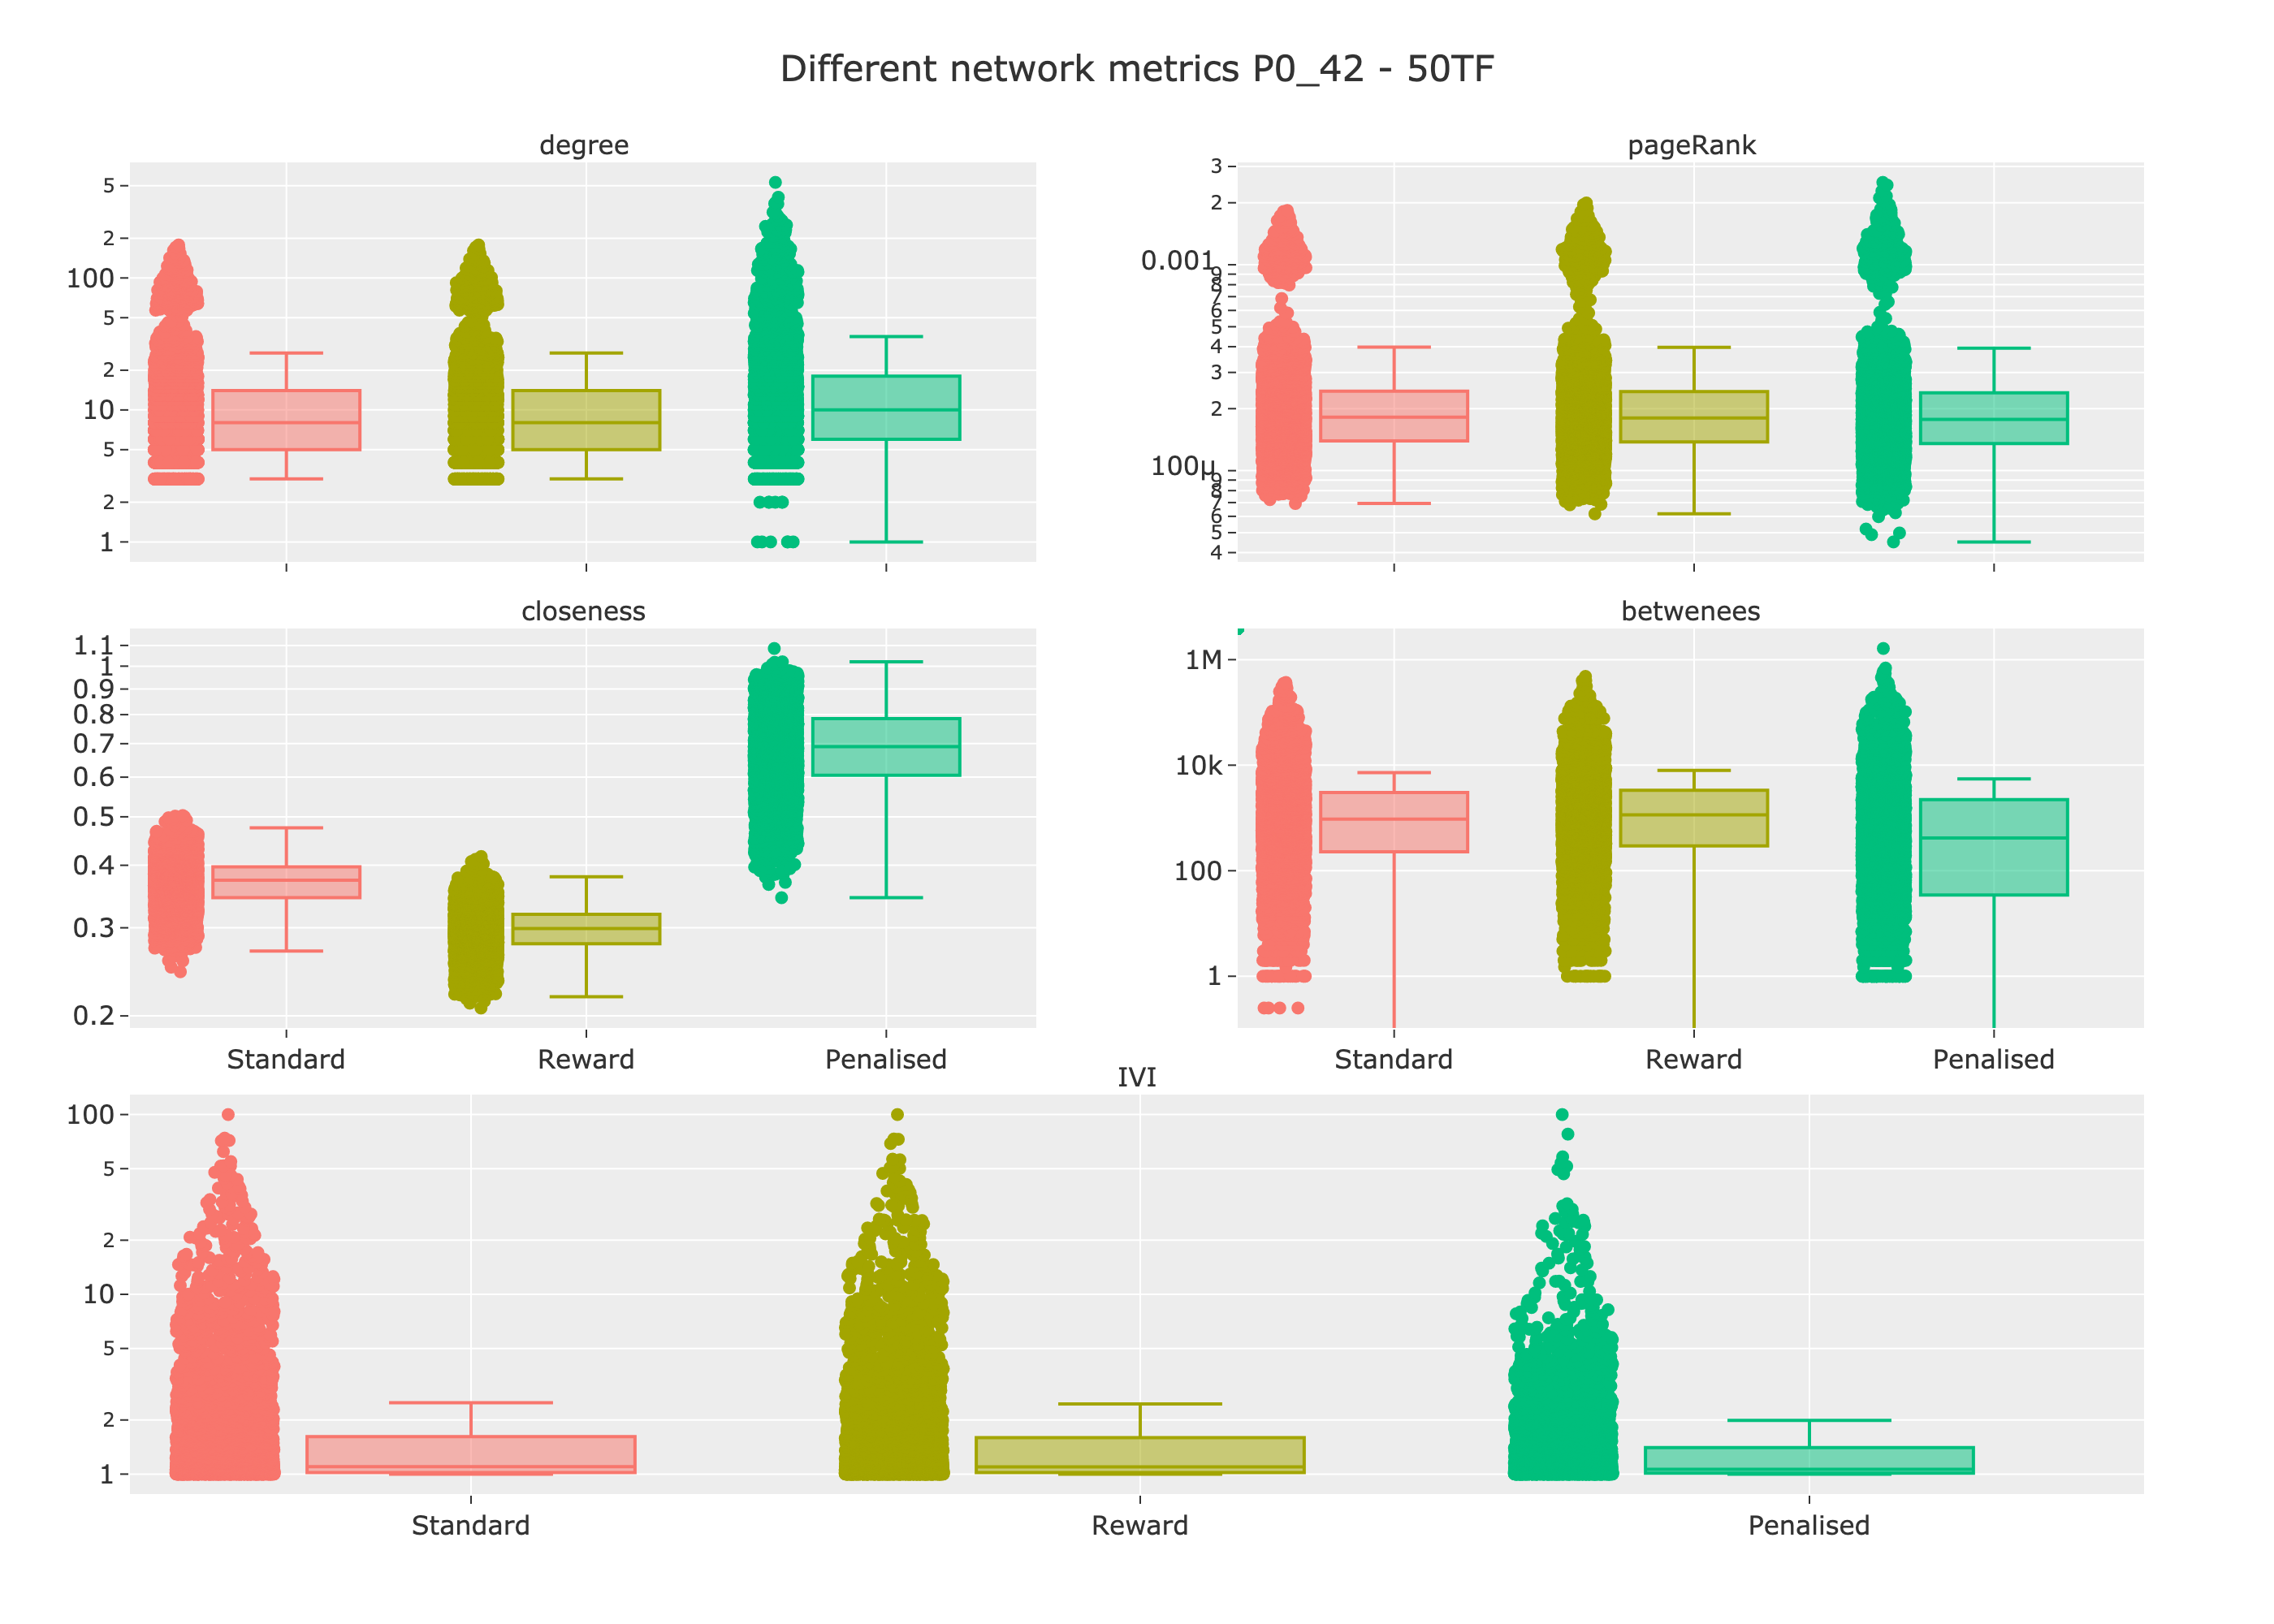
\includegraphics[width=1.0\textwidth,height=0.7\textheight,keepaspectratio]{Sections/Network_I/Resources/P0/P0_NetworkMetricsComp_50TF_2.png}
    \caption{Network metrics for the P0 networks formed from 4K genes, 3 connections per standard gene and 50 for TFs with the different weight modifiers; standard (blue), reward (red) and penalised (green). The y-axis represent the log10 of the metric. }
    \label{fig:N_I:net_metrics_p0}
\end{figure}

In the previous section \ref{s:N_I:tum_describe} five different network metrics were chosen to describe the networks generated: degree, PageRank, closeness, betweeness and IVI. These give an overview of the network properties, how well are the nodes connected, shortest path between them and their overall importance (IVI). In Figure \ref{fig:N_I:net_metrics_p0} the degree and PageRank plots for Standard and Reward network have a con-like set of points, denoting a subgroup of genes with a high number of edges. This is further enforced by the scale of the Y-axes; compared to the tumour experiments where the nodes degree where <100. Interestingly, PageRank values are at the similar scale with the ones from the tumour experiments (Figure \ref{fig:N_I:net_metrics_tum}). From the Closeness plot it can be seen that the Reward and Standard have lower values compared to Penalised denoting that less central nodes in the networks. For the Integrated Value Of Influence (IVI) the Standard and Reward have a larger spread compared to Penalised. 

Overall, the network metrics suggest that the Penalised network is different from the other two networks suggesting that reducing the weights to values close to 0 for highly mutated genes has a higher impact on the network than doubling their values.

\subsubsection{Choosing Clustering model}

% Explain what and why are the clustering methods we used
To find the appropriate clustering model and the number of clusters we adapt the previous work done in Chapter \ref{} (Subtyping chapter) where we used Principal Component Analysis (PCA) and K-means to stratify MIBC based on gene expression. Based on three different clustering method (Silhouette with cosine distance, Calinski Habrasz and Davies Bouldin\footnote{For a refresher on the clustering metrics see Section \ref{}}) we selected following clustering models \footnote{I have explored other clustering methods such as DBSCAN, MeanShit, Affinity Propagation, OPTICS, HDBSCAN and Fuzzy K-means. All based on Scikit-learn \cite{Scikit-learn_undated-ax}} the K-means, Agglomerative Clustering with Average linkage (Agg\_Avg), Birch, Ward, Gaussian Mixture Model and Spectral Clustering. 

\begin{figure}[!htb]
    \centering
    \begin{subfigure}[b]{0.49\textwidth}
        \centering
        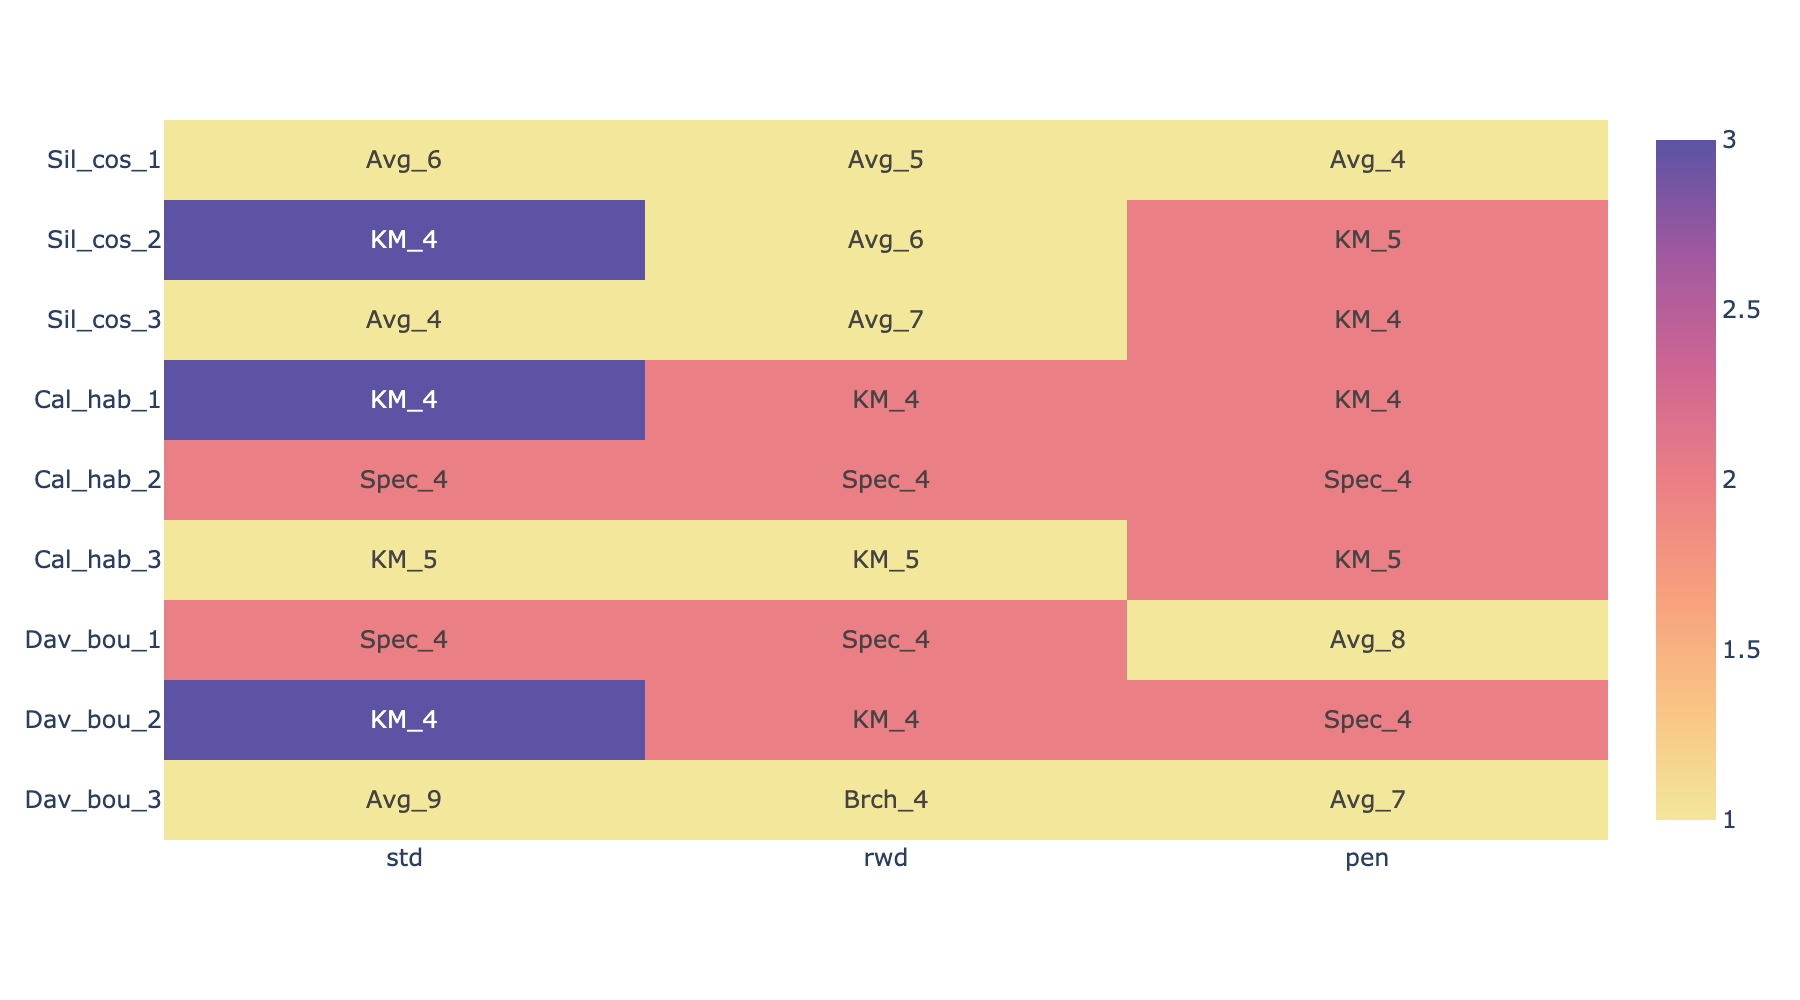
\includegraphics[width=\textwidth,keepaspectratio]{Sections/Network_I/Resources/P0/top3_cs_gen_p0_tum4K.png}    
        \caption{Cluster model and size}
    \end{subfigure}
    \hfill
    \begin{subfigure}[b]{0.49\textwidth}
        \centering
        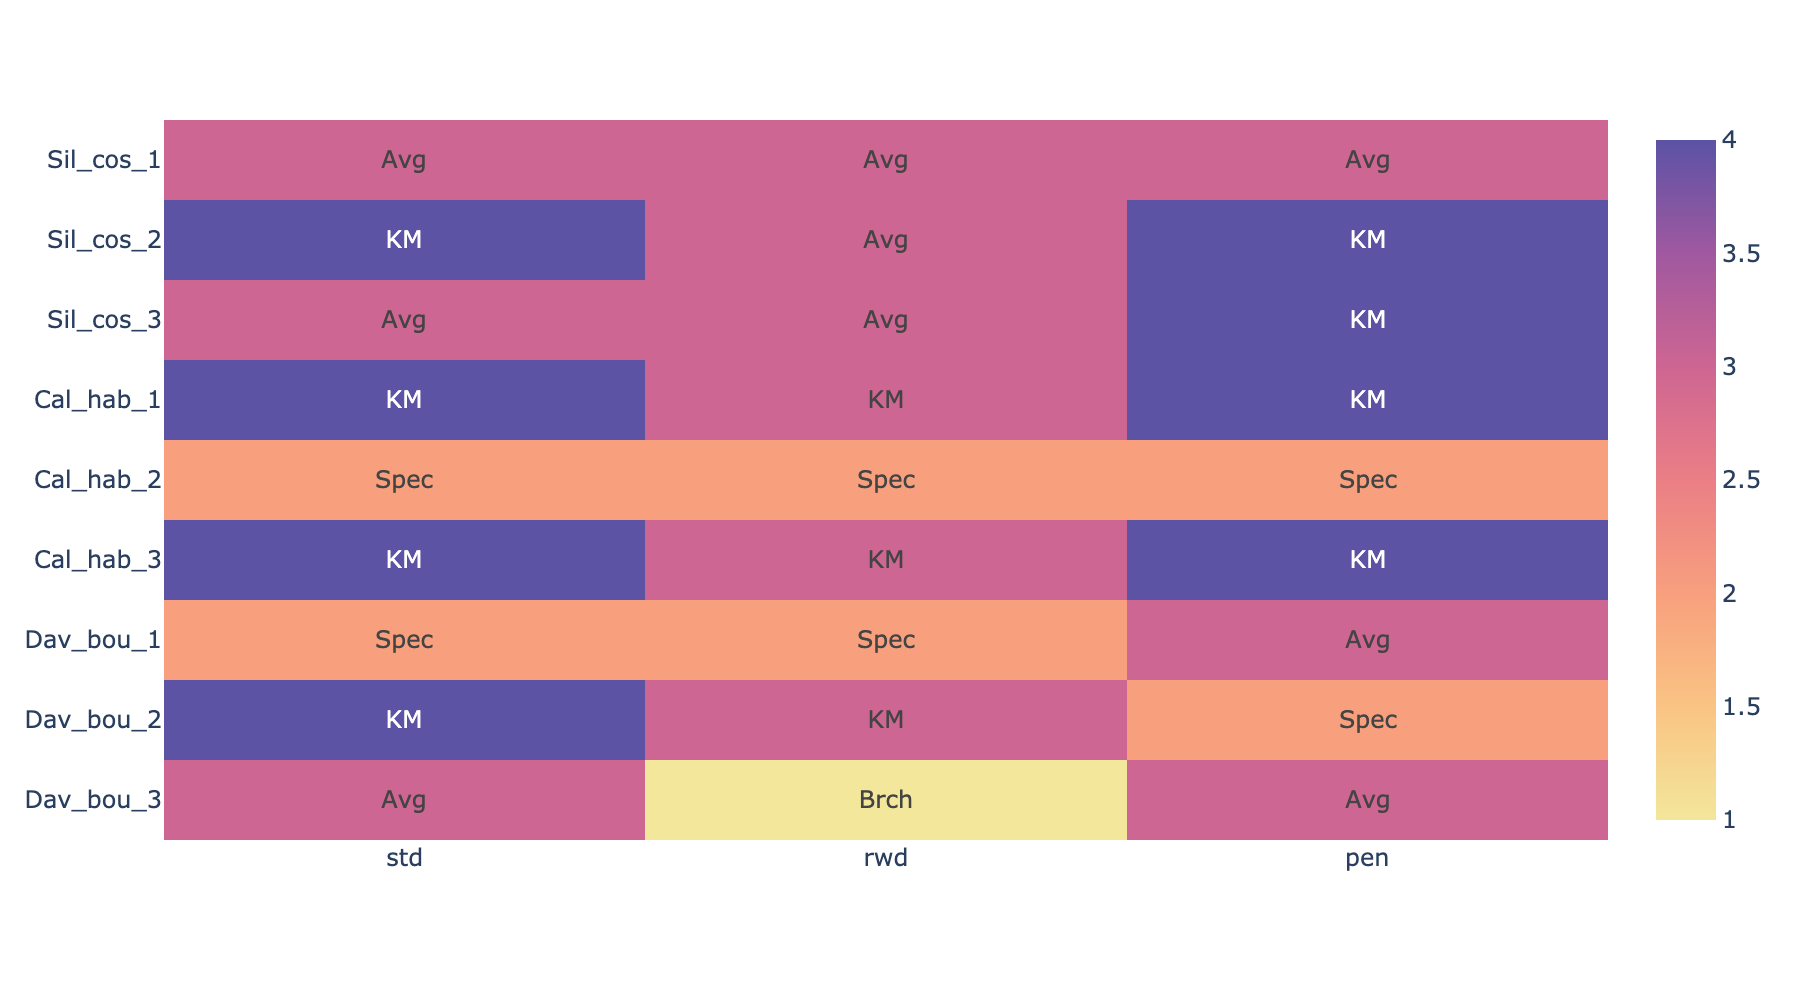
\includegraphics[width=\textwidth,keepaspectratio]{Sections/Network_I/Resources/P0/top3_cs_model_p0_tum4K.png}
        \caption{Cluster model}
    \end{subfigure} %
    \hfill
    \begin{subfigure}[b]{0.49\textwidth}
        \centering
        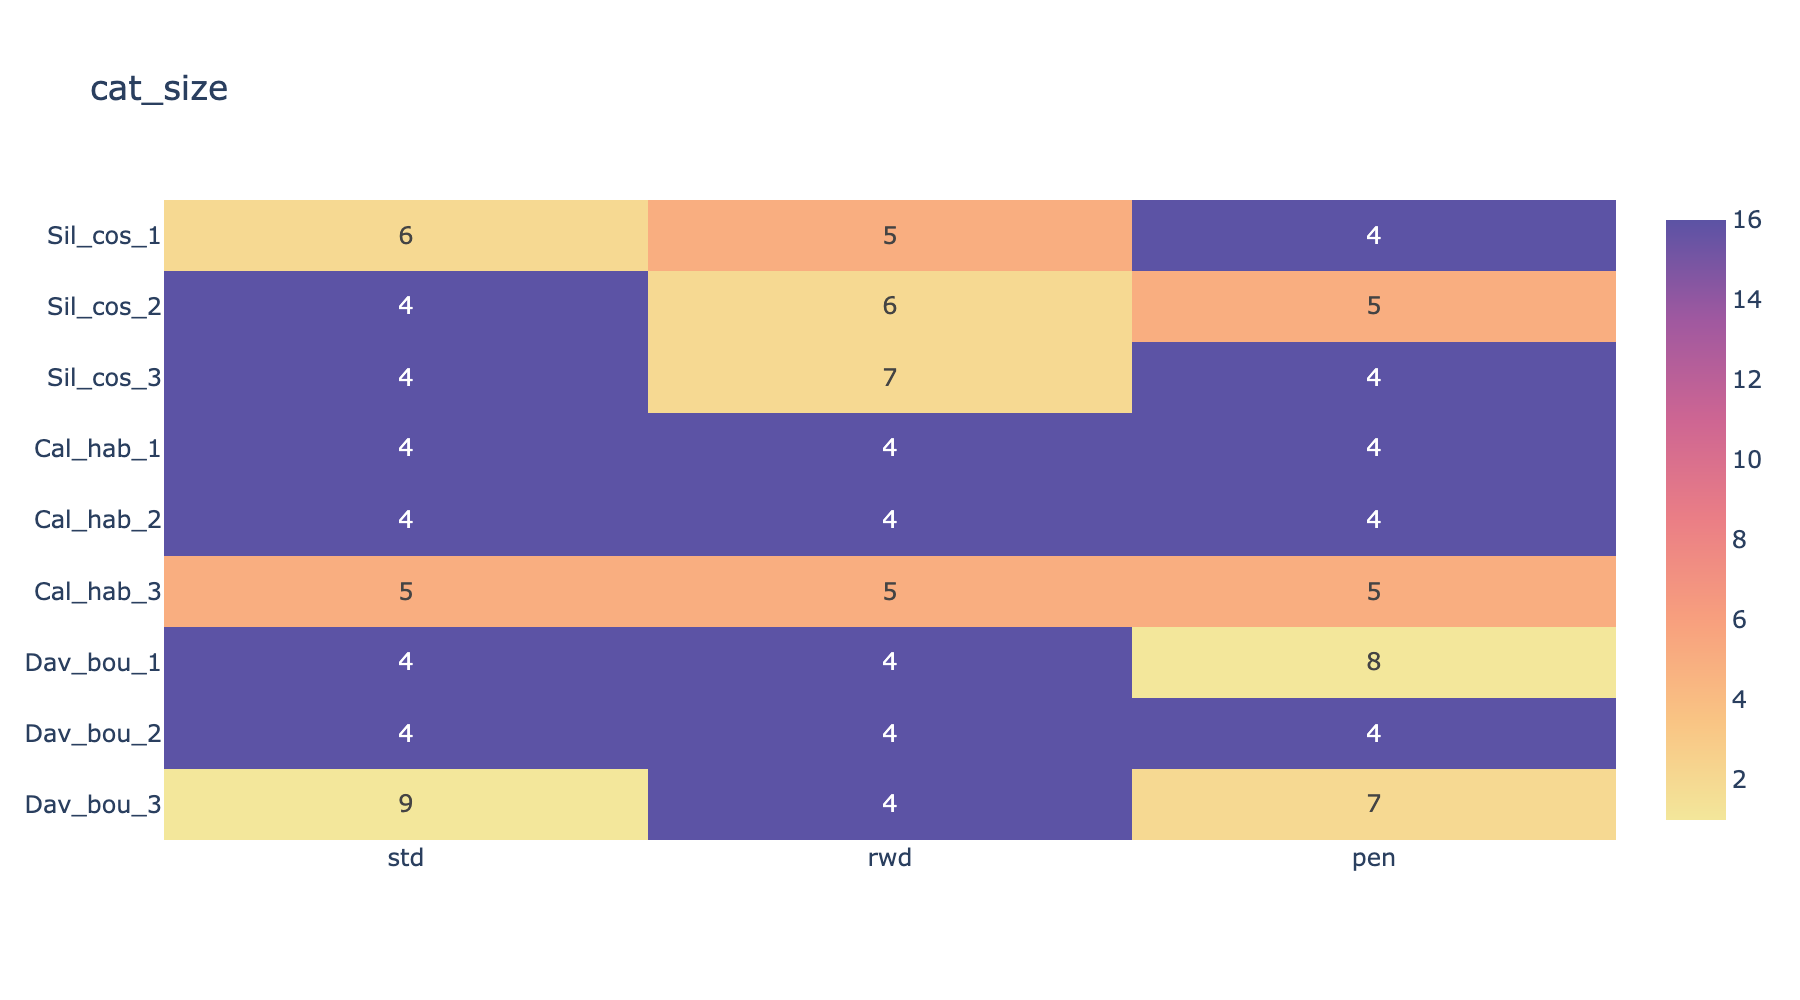
\includegraphics[width=\textwidth,keepaspectratio]{Sections/Network_I/Resources/P0/top3_cs_size_p0_tum4K.png}
        \caption{Cluster size}
    \end{subfigure}
     \hfill
    \begin{subfigure}[b]{0.49\textwidth}
        \centering
        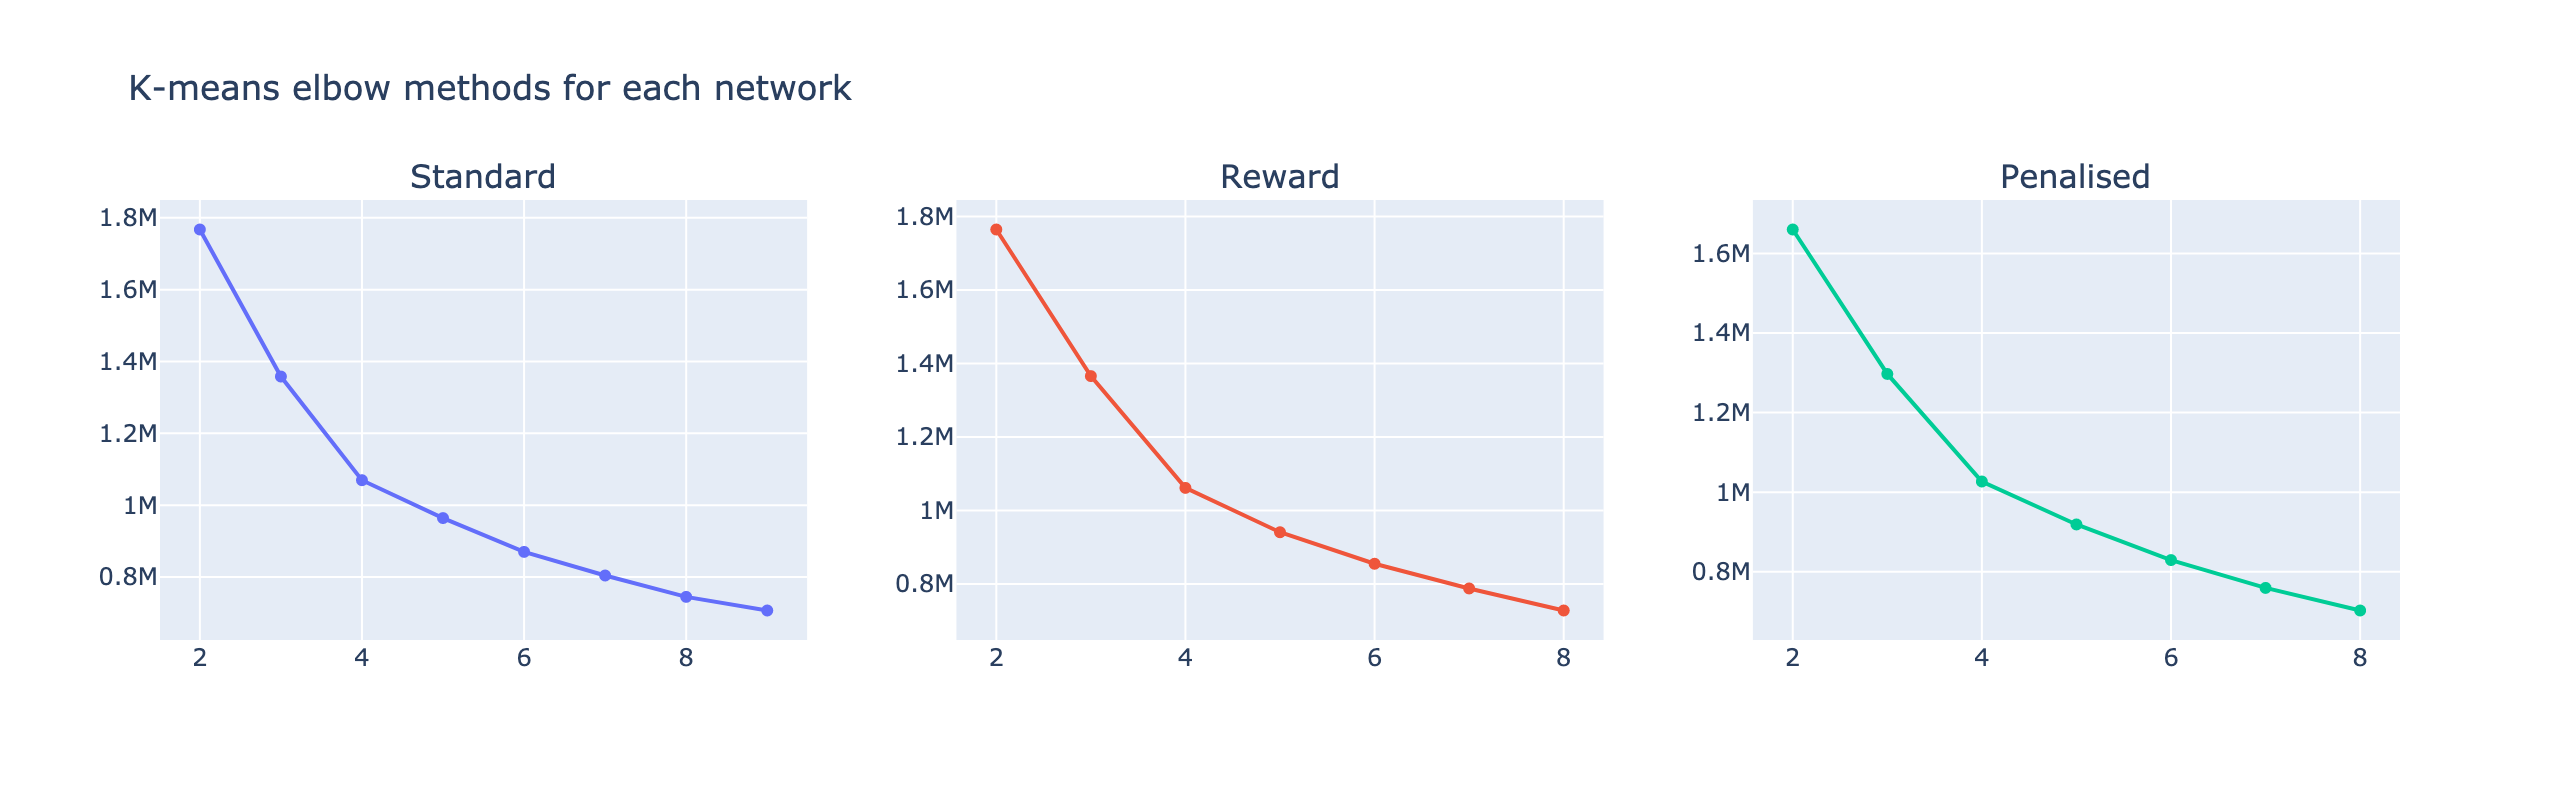
\includegraphics[width=\textwidth, keepaspectratio]{Sections/Network_I/Resources/P0/p0_elbowMethod_4K.png}
        \label{fig:N_I:p0_elbow_method}
        \caption{Elbow method}
    \end{subfigure}
    \caption{Clustering models for each network type with the top three clustering scores. Colouring scale corresponds to the encounter frequency \textbf{per network type}; i.e. the count restarts for every network. A) looks at the overall most common clustering model configuration. B) at the most common clustering model C) the most likely cluster size.}
    \label{fig:N_I:p0_top_3_metrics}
\end{figure}


% Introduce the results and motivate the reason of why we don't include K=2,3
In this section we apply the above-mentioned clustering methods to the MEV scores derived from the three networks (Standard, Reward and Penalised) with K ranging from 3-9 and we used the same clustering metrics to assess the performance. In Figure \ref{fig:N_I:p0_choosing_cs} the clustering metrics are displayed, were the number of 'x' marks the highest score after cluster size 2 and 3. The models with 2 clusters or 3 are not taken in account as the metrics tend to give higher score for models with 2,3 clusters. This can be seen in our results as well were usually the clustering models perform worst with the increase of K. 

\begin{figure}[!htb]
    \thispagestyle{plain}
    \centering
    \begin{subfigure}{1.0\linewidth}
        \centering
        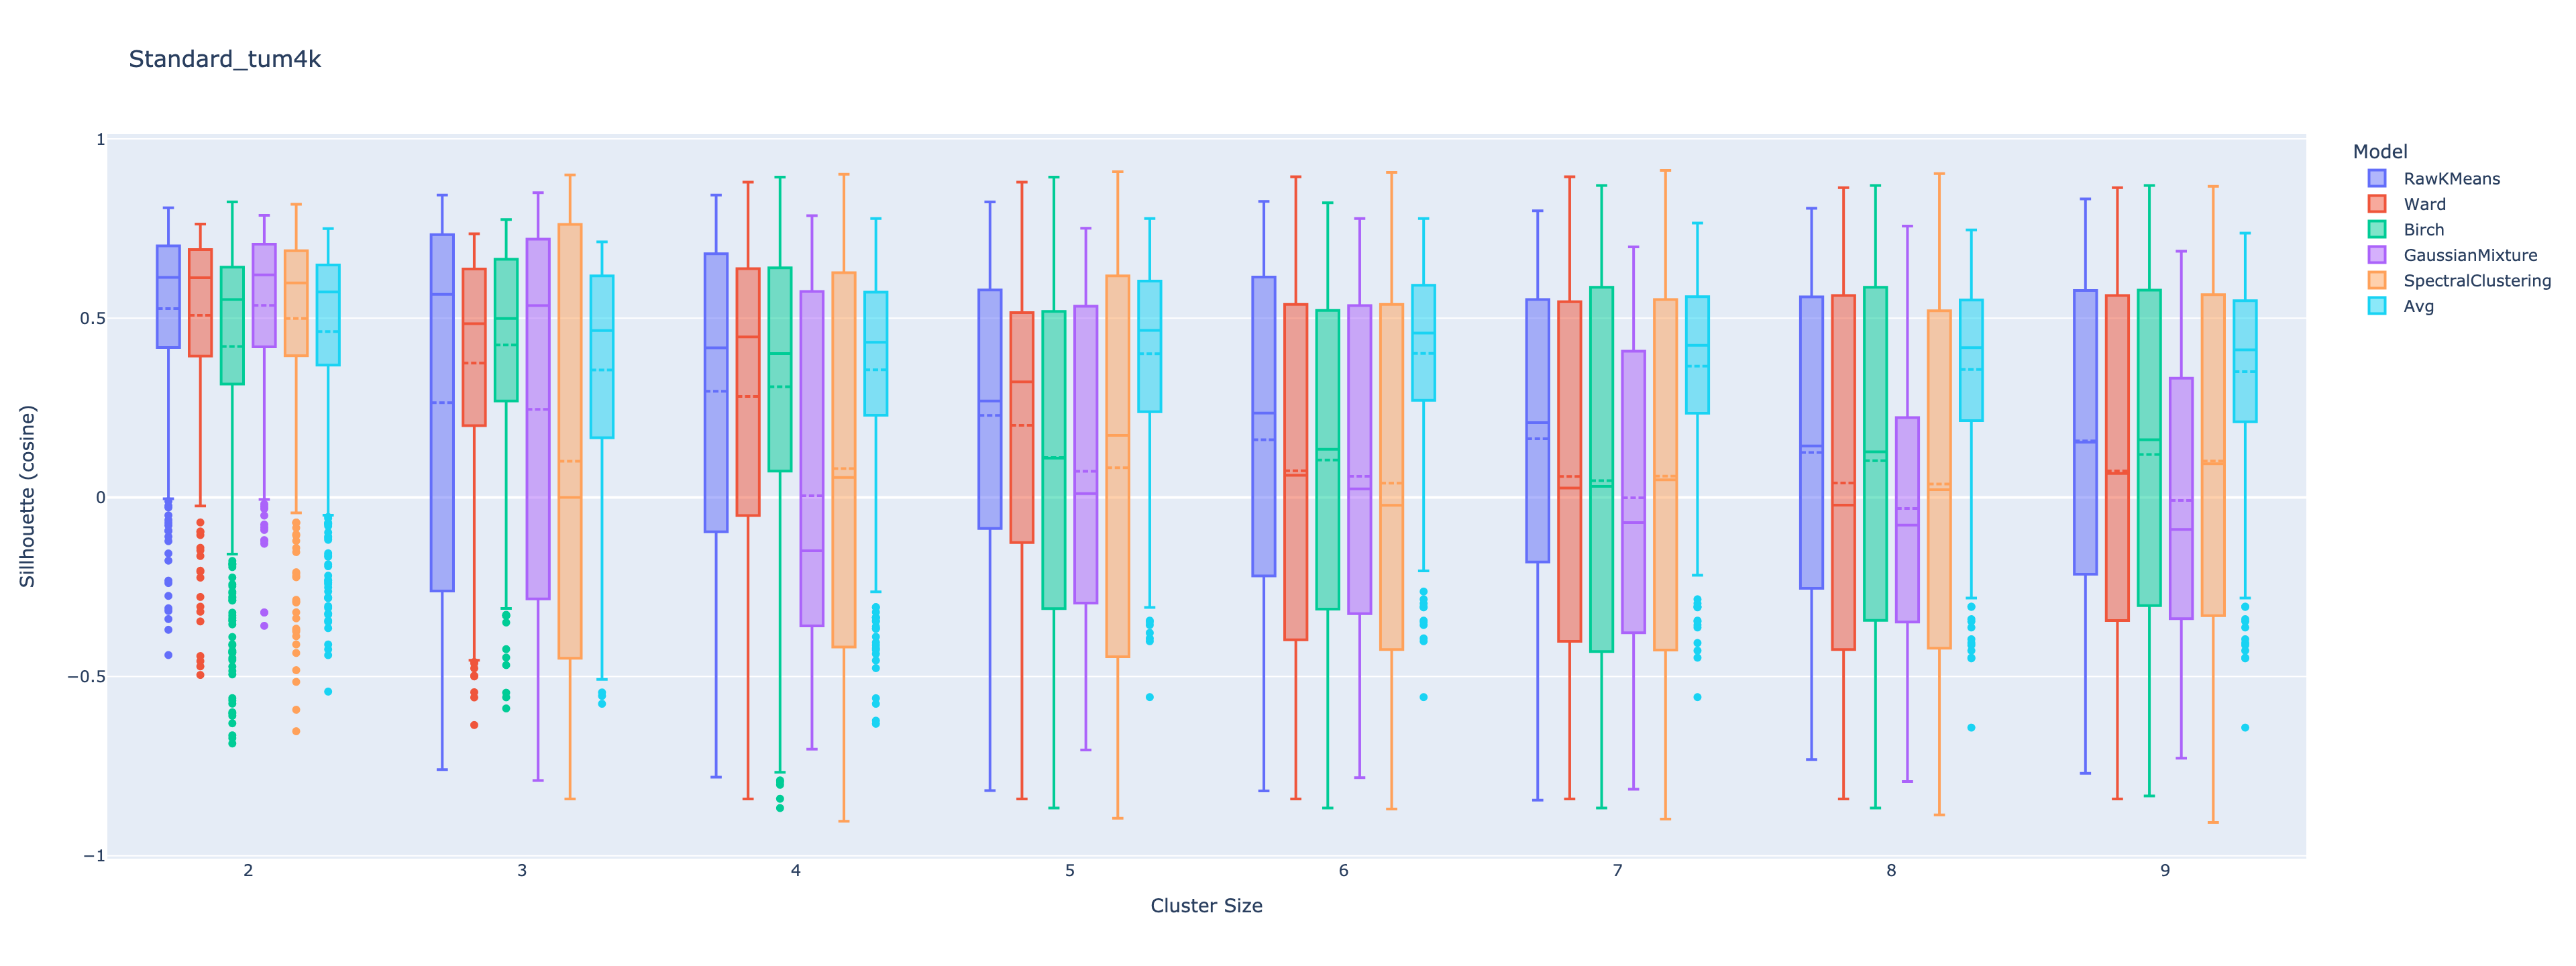
\includegraphics[width=1.0\textwidth,height=0.17\textheight]{Sections/Network_I/Resources/P0/Standard_tum4k_sill_spread.png}
        \caption{Standard network}
    \end{subfigure} %

    \begin{subfigure}{1.0\linewidth}
        \centering
        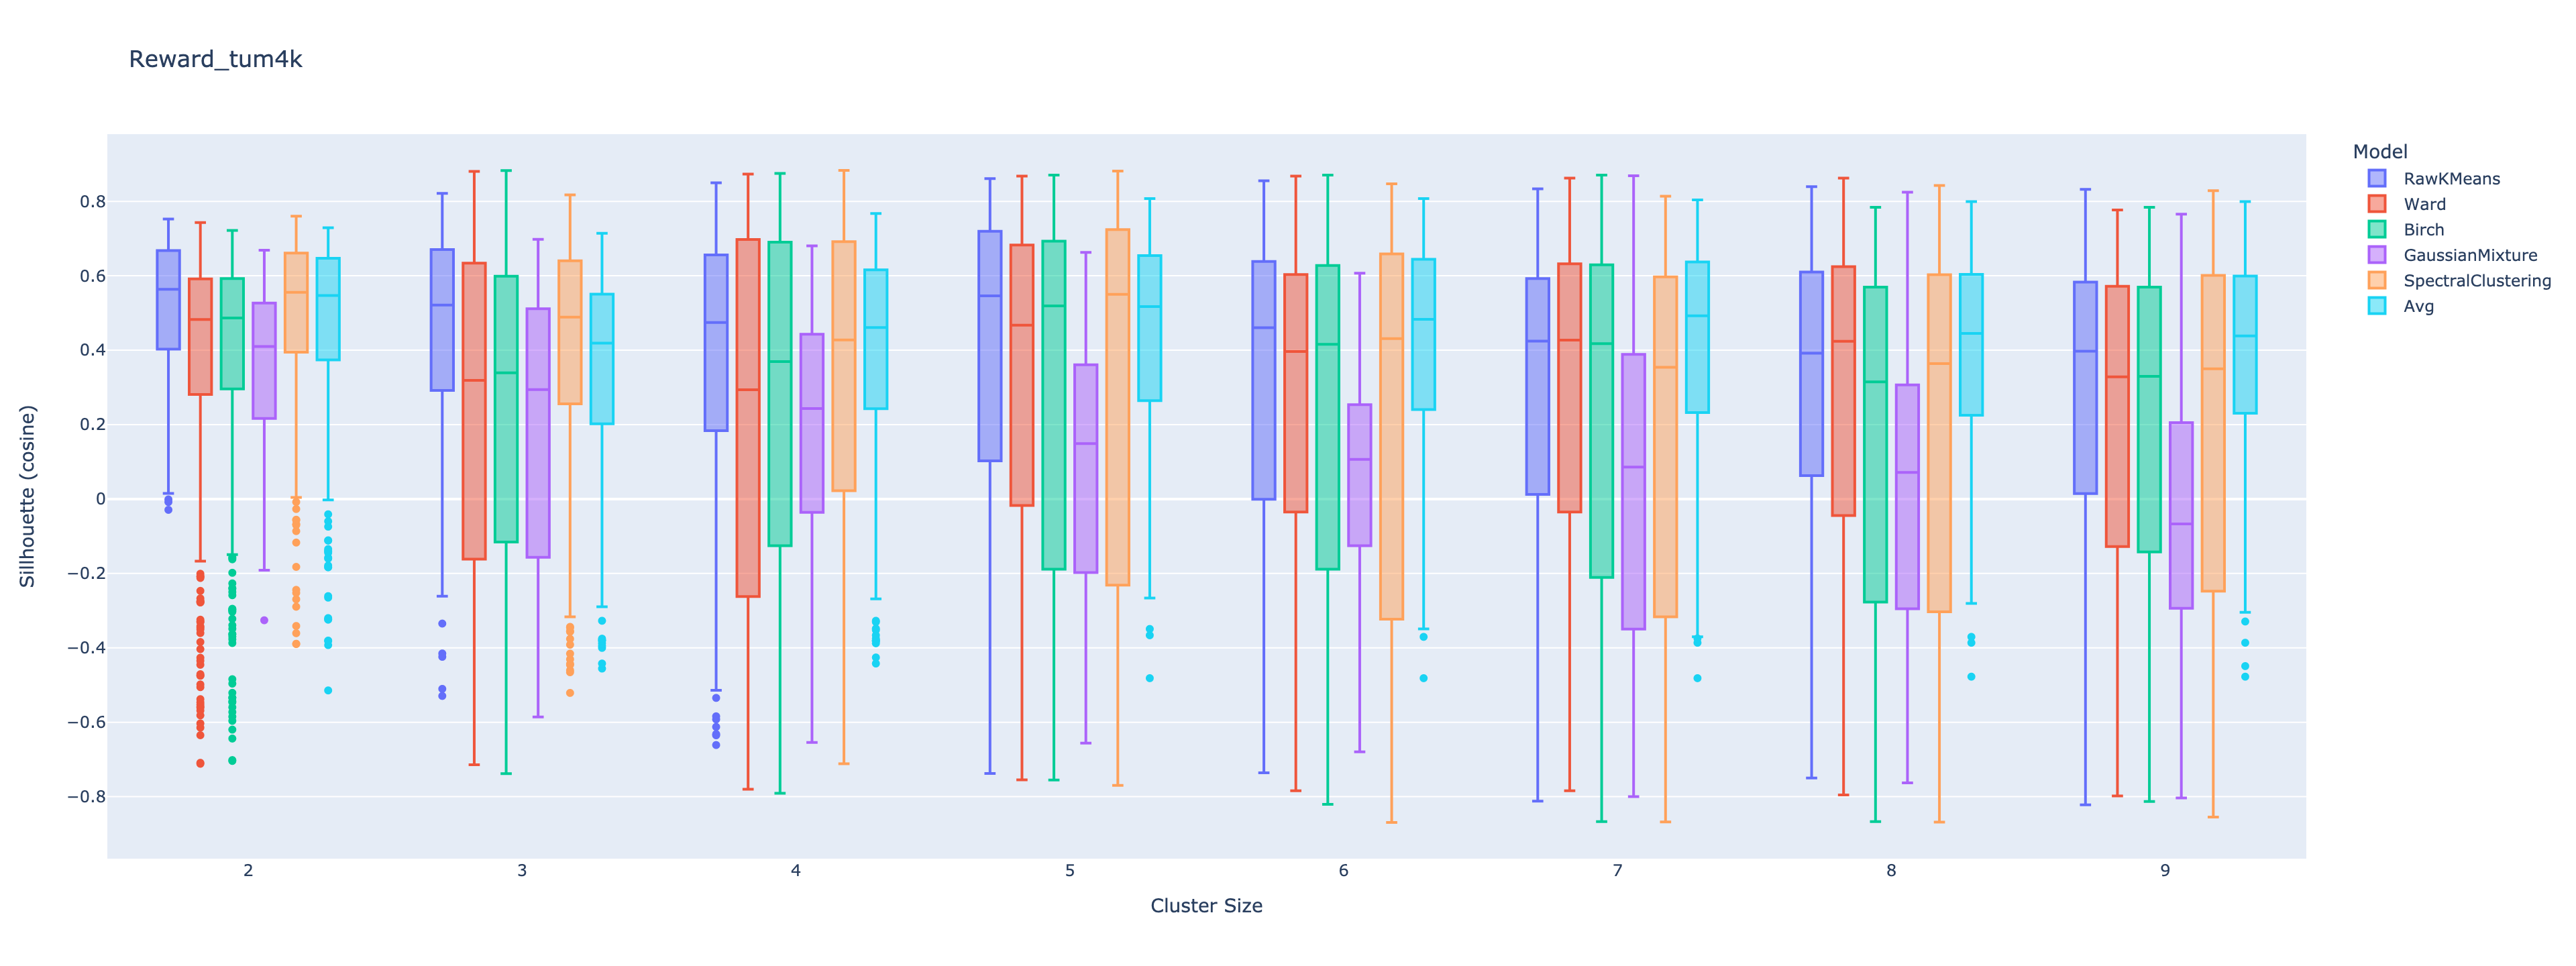
\includegraphics[width=1.0\textwidth,height=0.17\textheight]{Sections/Network_I/Resources/P0/Reward_tum4k_sill_spread.png}
        \caption{Reward network}
    \end{subfigure}
    
    \begin{subfigure}{1.0\linewidth}
        \centering
        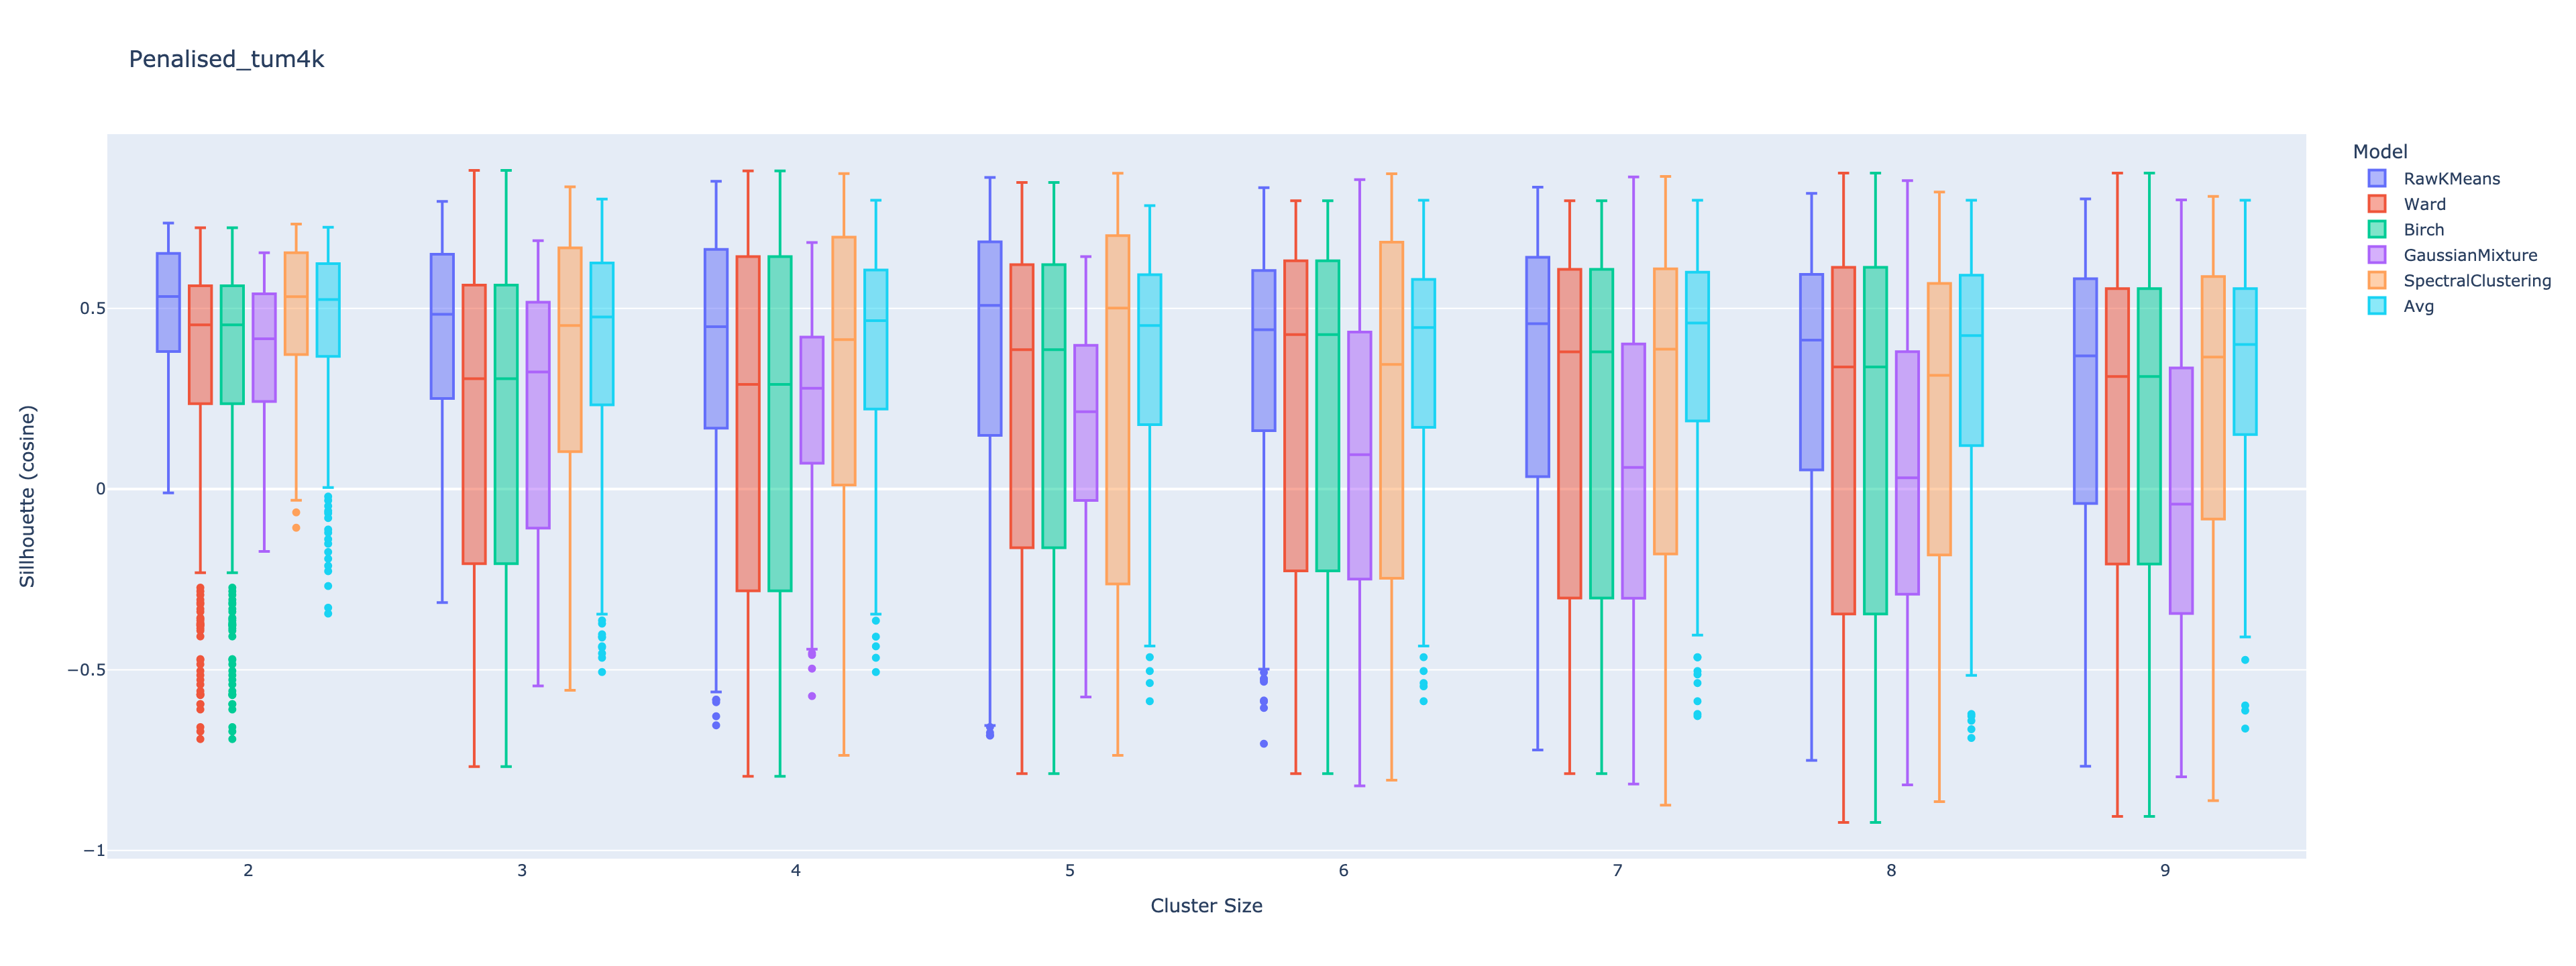
\includegraphics[width=1.0\textwidth,height=0.17\textheight]{Sections/Network_I/Resources/P0/Penalised_tum4k_sill_spread.png}      
        \caption{Penalised network}
    \end{subfigure}
    \caption{Cosine Silhouette score spread across samples over different clustering models with various K.}
    \label{fig:N_I:p0_sillhouette_spread}
\end{figure}

\begin{figure}[!htb]
    \hfill
    \begin{subfigure}{1.0\linewidth}
        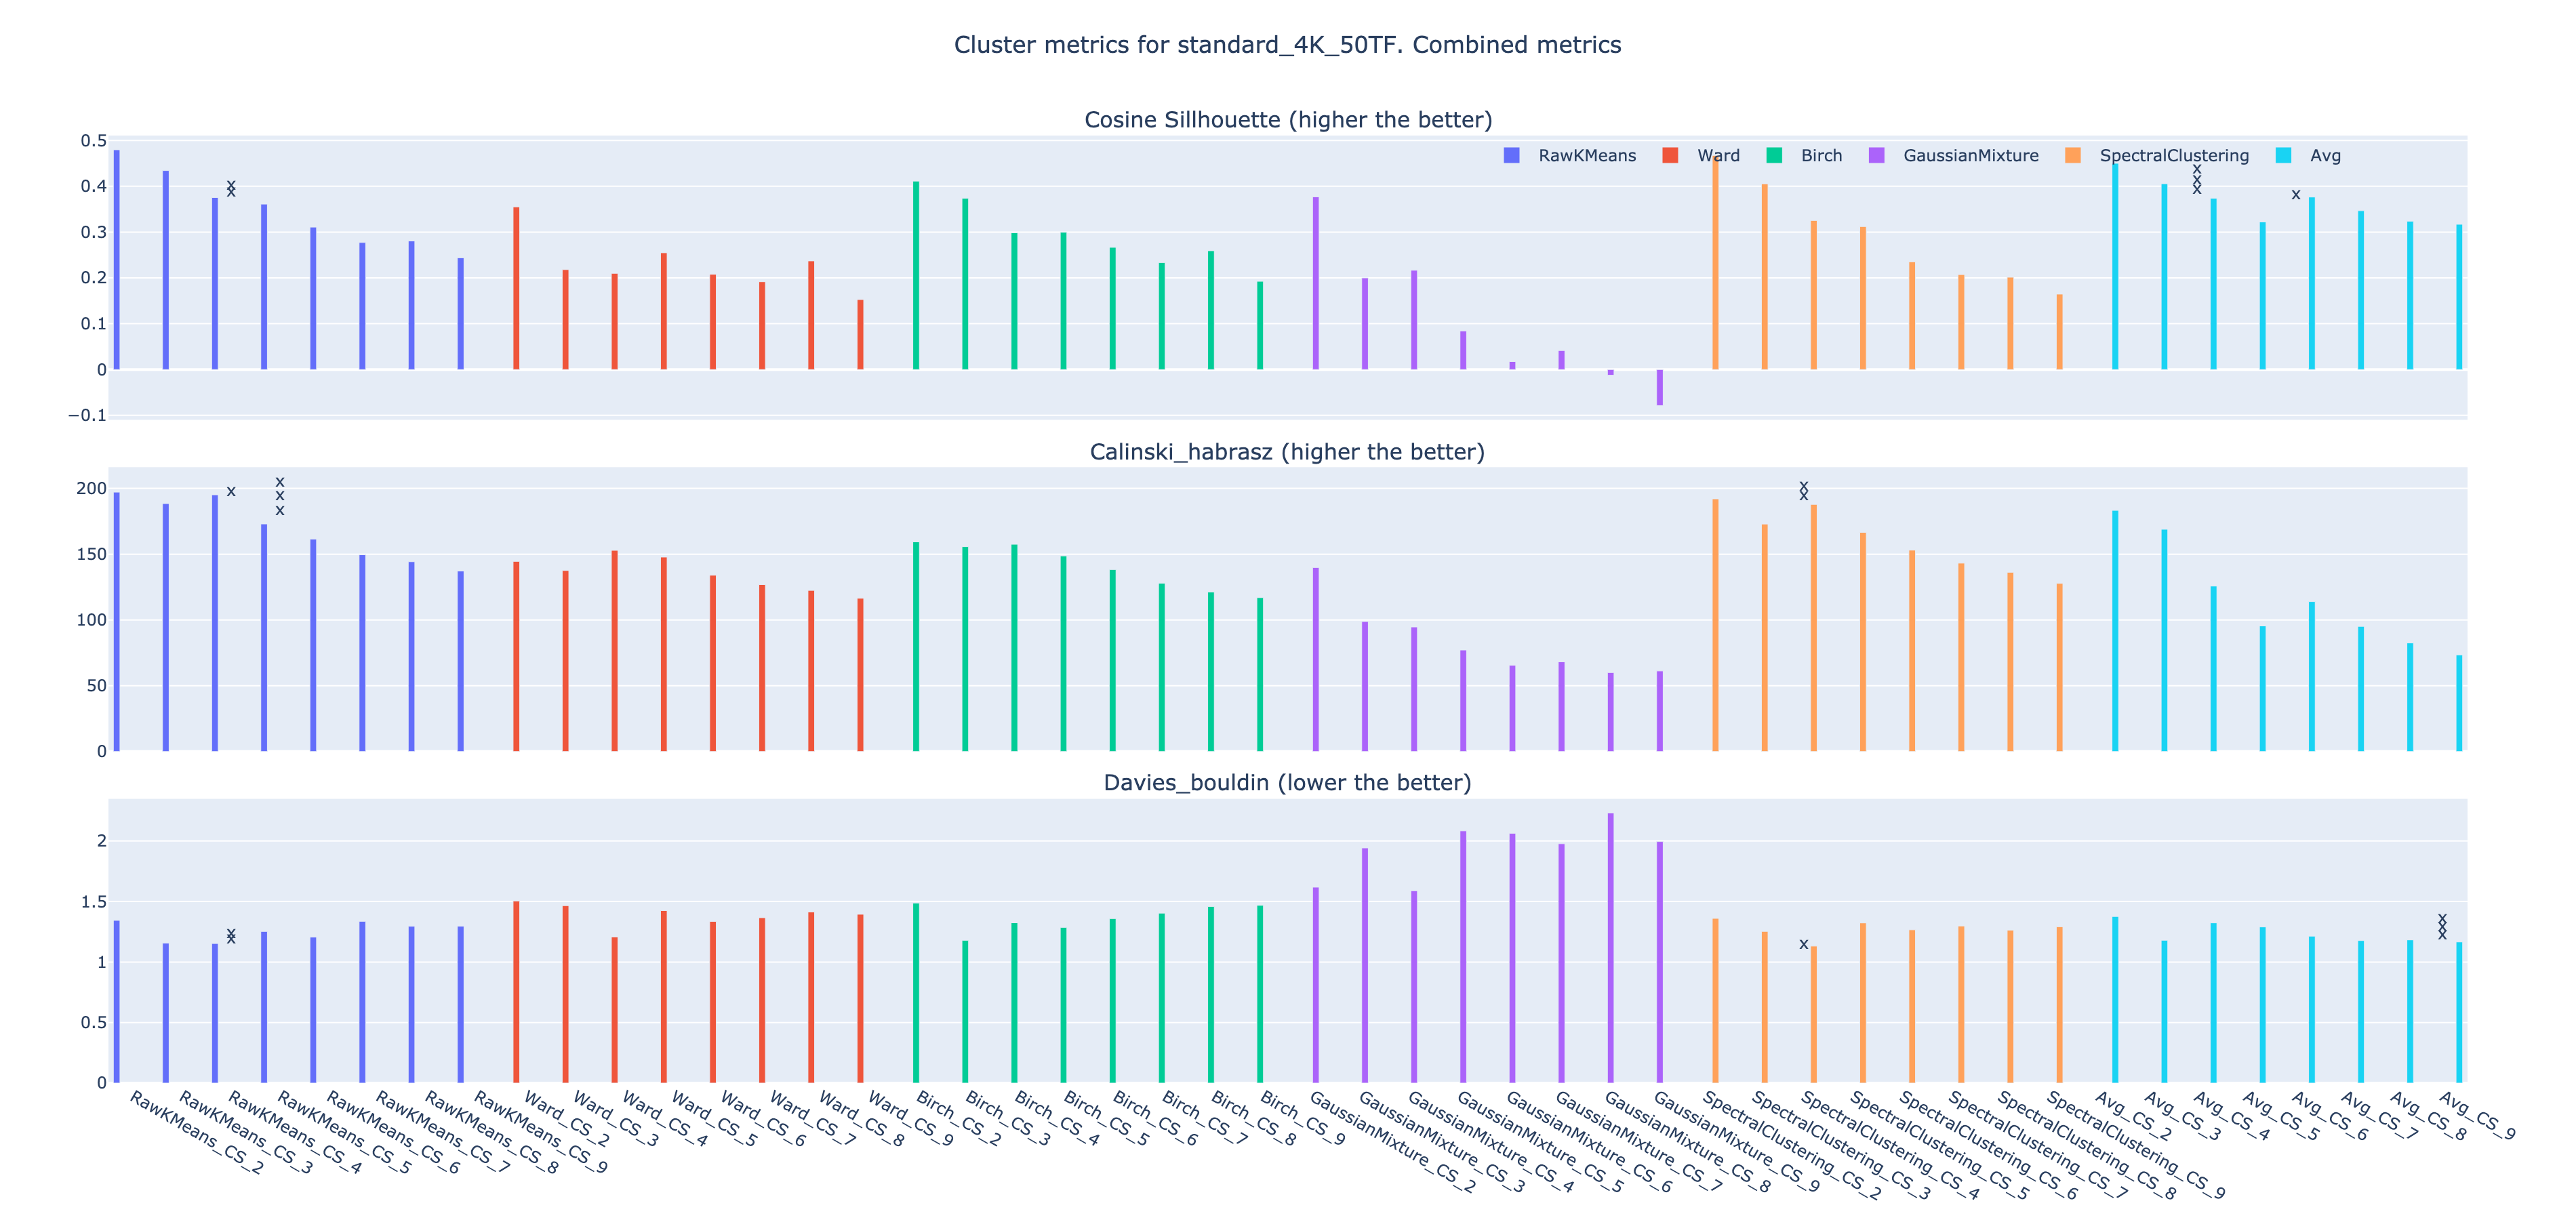
\includegraphics[width=1.0\textwidth,height=0.25\textheight]{Sections/Network_I/Resources/P0/CA_metrics_Std_2_tum_4k.png}
        \caption{Standard network}
    \end{subfigure} %
    \hfill
    \begin{subfigure}{0.49\linewidth}
        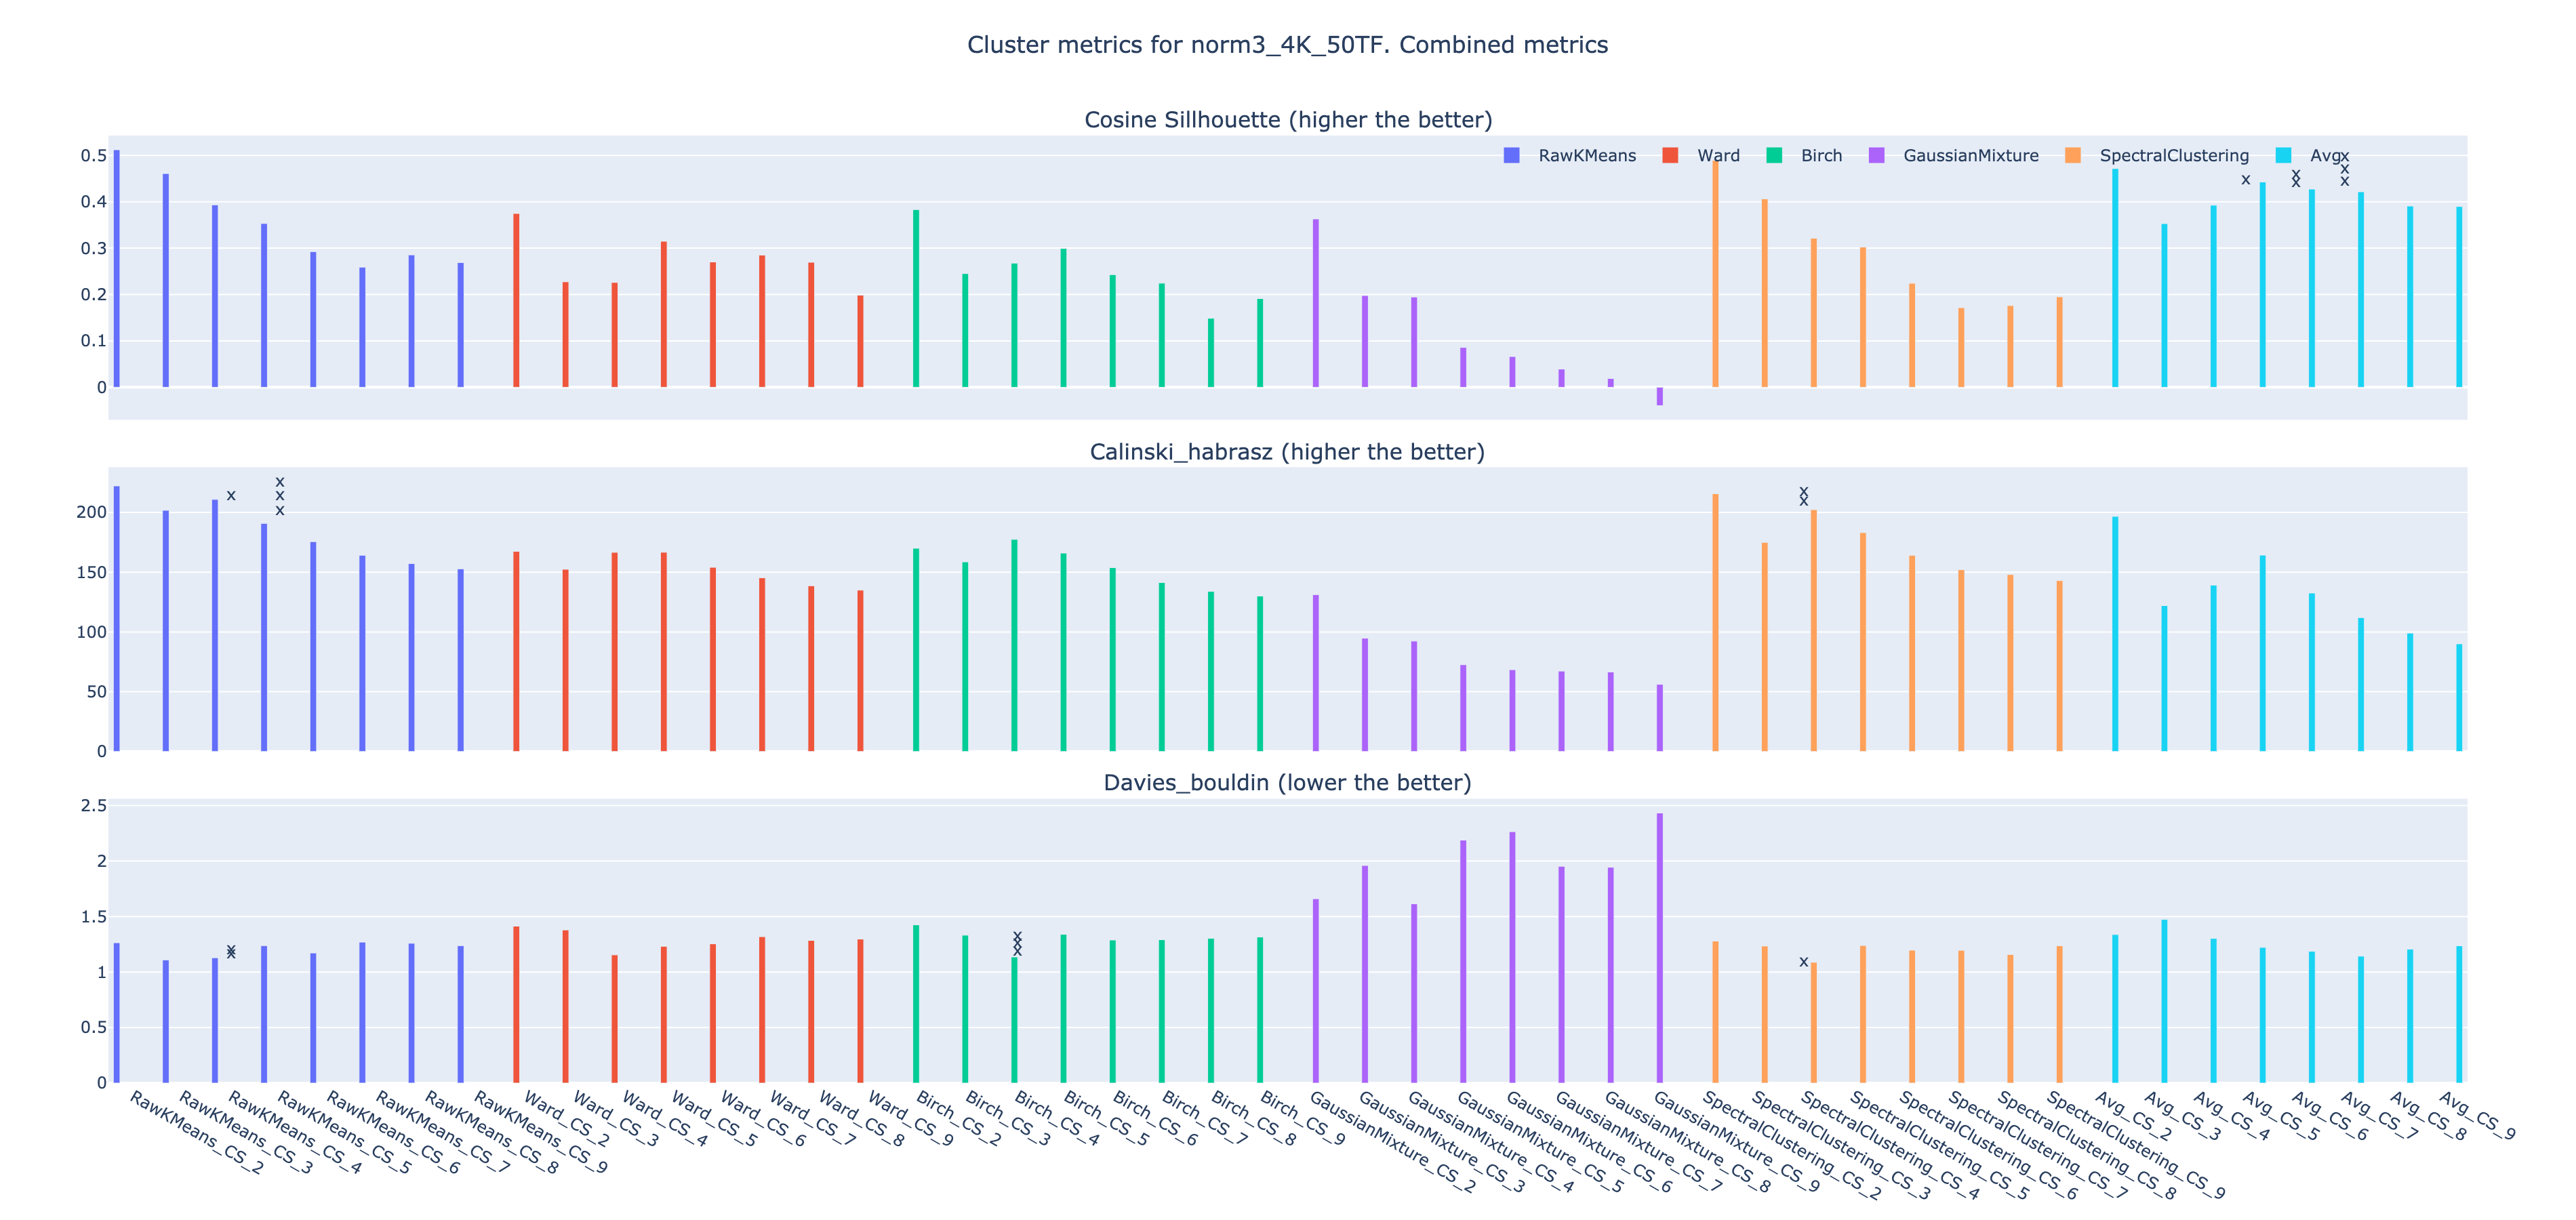
\includegraphics[width=1.0\textwidth,height=0.25\textheight]{Sections/Network_I/Resources/P0/CA_metrics_Rwd_2_tum_4k.png}
        \caption{Reward network}
    \end{subfigure}
    \hfill
    \begin{subfigure}{0.49\linewidth}
        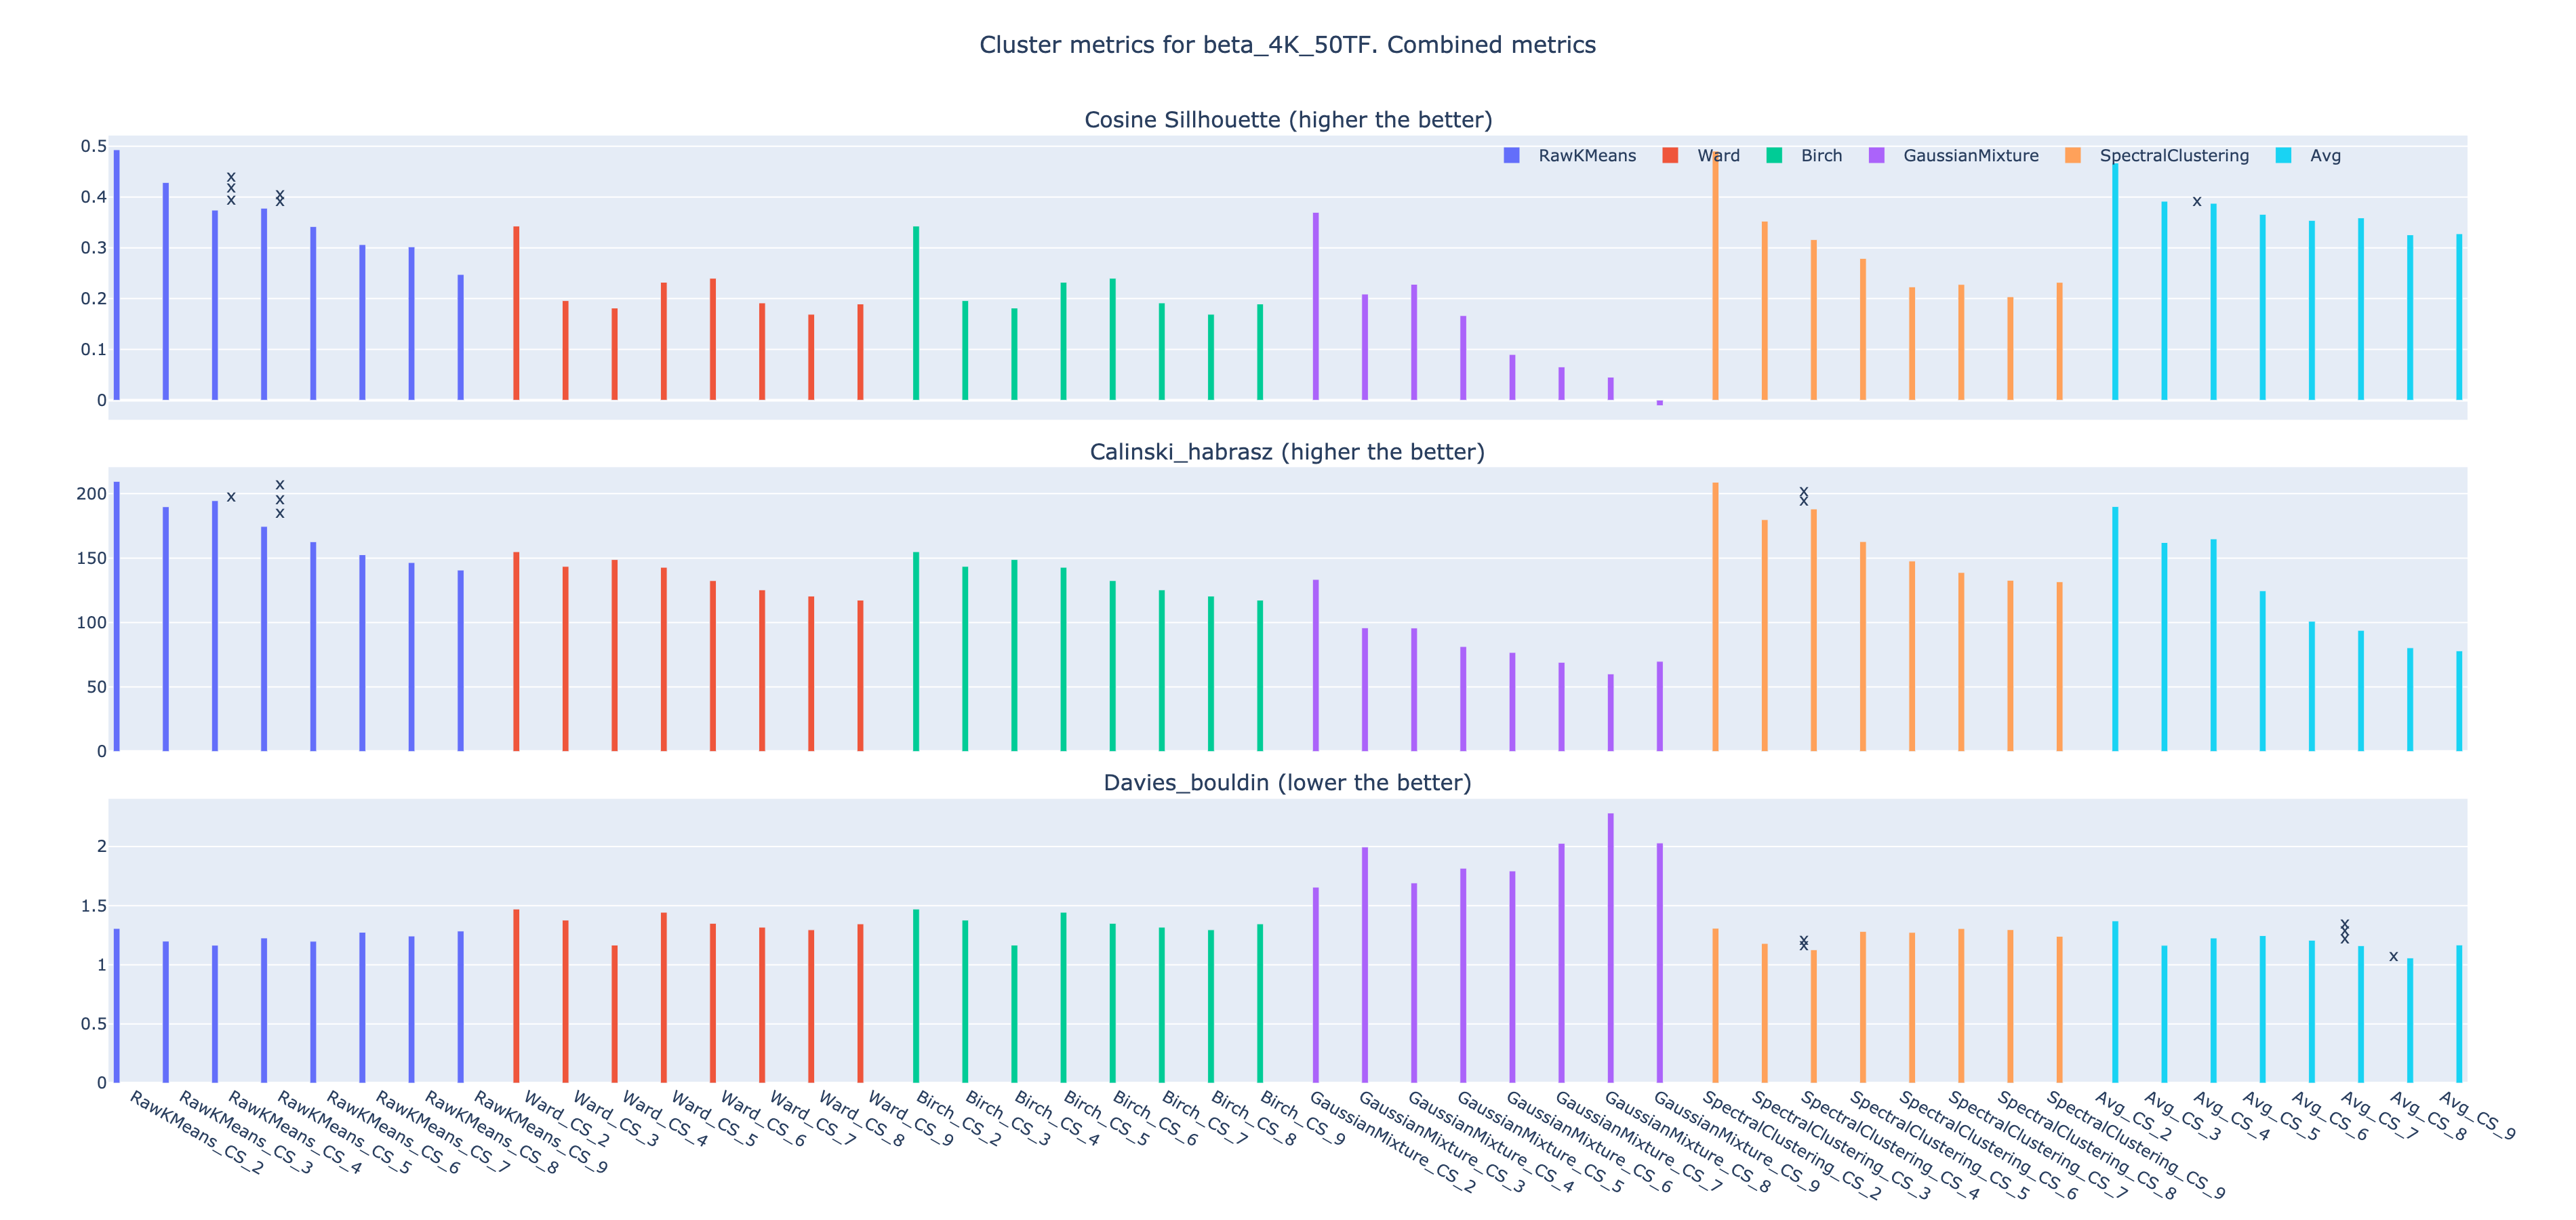
\includegraphics[width=1.0\textwidth,height=0.25\textheight]{Sections/Network_I/Resources/P0/CA_metrics_Pen_2_tum_4k.png}
        \caption{Penalised network}
    \end{subfigure}
    \hfill
    \caption{Clustering metrics for the 3 networks generated from P0 samples.}
    \label{fig:N_I:p0_choosing_cs}
\end{figure}


% Comment on Top 3 models + cs, models and just CS
While Figure \ref{fig:N_I:p0_choosing_cs} shows the general trends of the metrics across the 3 different clustering scores, it is not very clear which model with how many clusters performs the best for each network or overall. Figure \ref{fig:N_I:p0_top_3_metrics} assists the decision making by looking at the most overall used model with cluster size, only at the cluster model and size in A), B) and C); the colouring scale corresponds to the encounter frequency across network type; e.g. in A) K-means with K=4 appears 3 times in standard network and Spectral Clustering with K=4 two times in all three network types. The colouring strategies helps delineating the configurations for each network. From Figure \ref{fig:N_I:p0_choosing_cs} A) it can be noticed that the standard network is the only one having a model picked by all three metrics. In B) it is clearer that K-means is the preferred model by both standard and penalised network, while for Reward network both Agg\_Avg and K-means are selected 3 times. In terms of the the cluster sizes, in Figure \ref{fig:N_I:p0_choosing_cs} C), K=4 is the most common number of subgroups followed by K=5. Overall, the clustering scores suggest that both K-Means and Agg\_Avg have similar performances while the preferred cluster sizes is K=4 followed by K=5. Furthermore, K=4 is the overall choice of clusters numbers through the Elbow approach in Figure \ref{fig:N_I:p0_top_3_metrics} D.


% Using cosine sillhouette to look at the spread
The lack of an obvious cluster model shows the challenge of working with gene expression datasets. It also shows the limitation of using average scores for clustering metrics. Thus, we select the Silhouette cosine score\footnote{For the same reason as we chosen it as a main metric in the last chapter. Compared with the other metrics the Silhouette score uses cosine as a distance which is more suitable for high dimension data.} to look at the spread across samples in Figure \ref{fig:N_I:p0_sillhouette_spread}. With the exception of the Agg\_Avg and K-means the other clustering models have a higher spread of the silhouette across the different cluster size.

% narrowing done to the 2 clustering models
The clustering scores and the analysis performed suggests that K-means and Agglomerative Clustering with average linkage perform better than the rest as in the top 3 models used \ref{fig:N_I:p0_top_3_metrics} B) and the silhouette spread in Figure \ref{fig:N_I:p0_sillhouette_spread}. The Elbow method Figure \ref{fig:N_I:p0_top_3_metrics} D) and the other metrics suggests that K=4 is the right choice. This is different from what is expected as in the earlier work \ref{} we found at least five clusters using computational methods and K=6 with biological knowledge (IFNg groups). Also, this is is the next K considered as K=2,3 are not taken in account when finding the top 3 scores as it was explained at the beginning of the section.

\begin{figure}[!htb]
    \hfill
    \begin{subfigure}[b]{0.49\textwidth}
        \centering
        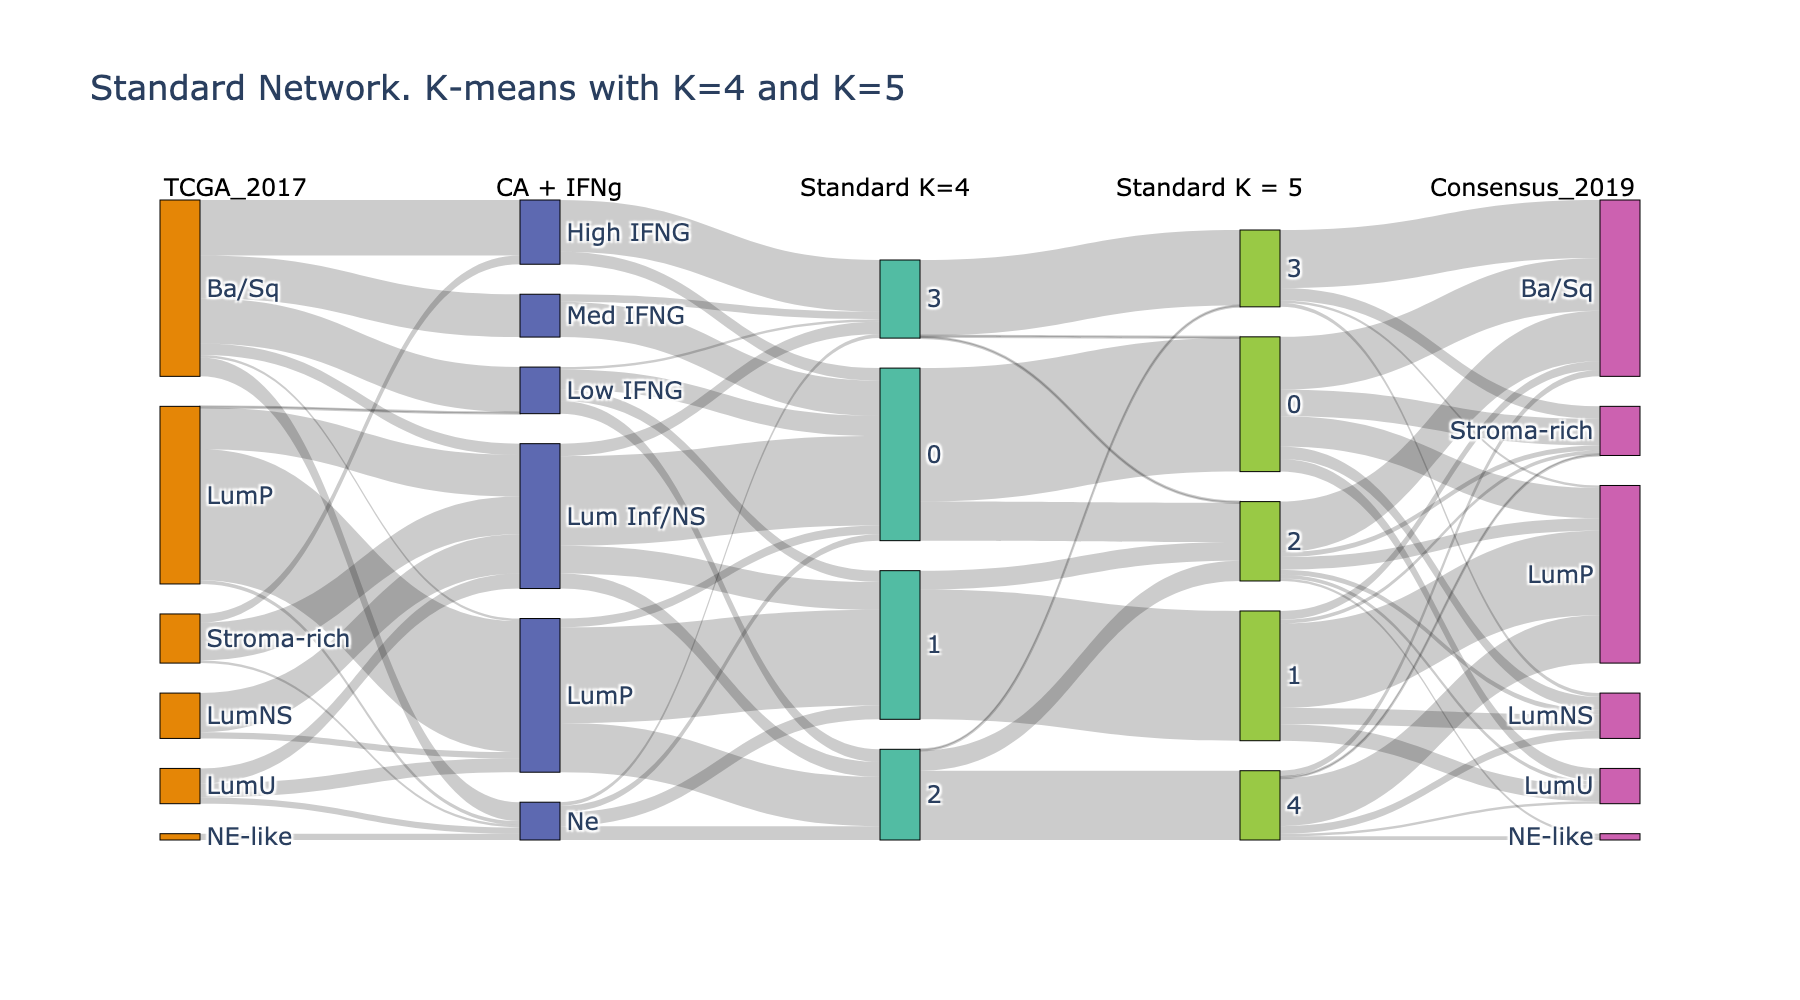
\includegraphics[width=\textwidth,keepaspectratio]{Sections/Network_I/Resources/P0/Sankey_KM_4K.png}
        \caption{K-Means}
    \end{subfigure}
    \hfill
    \begin{subfigure}[b]{0.49\textwidth}
        \centering
        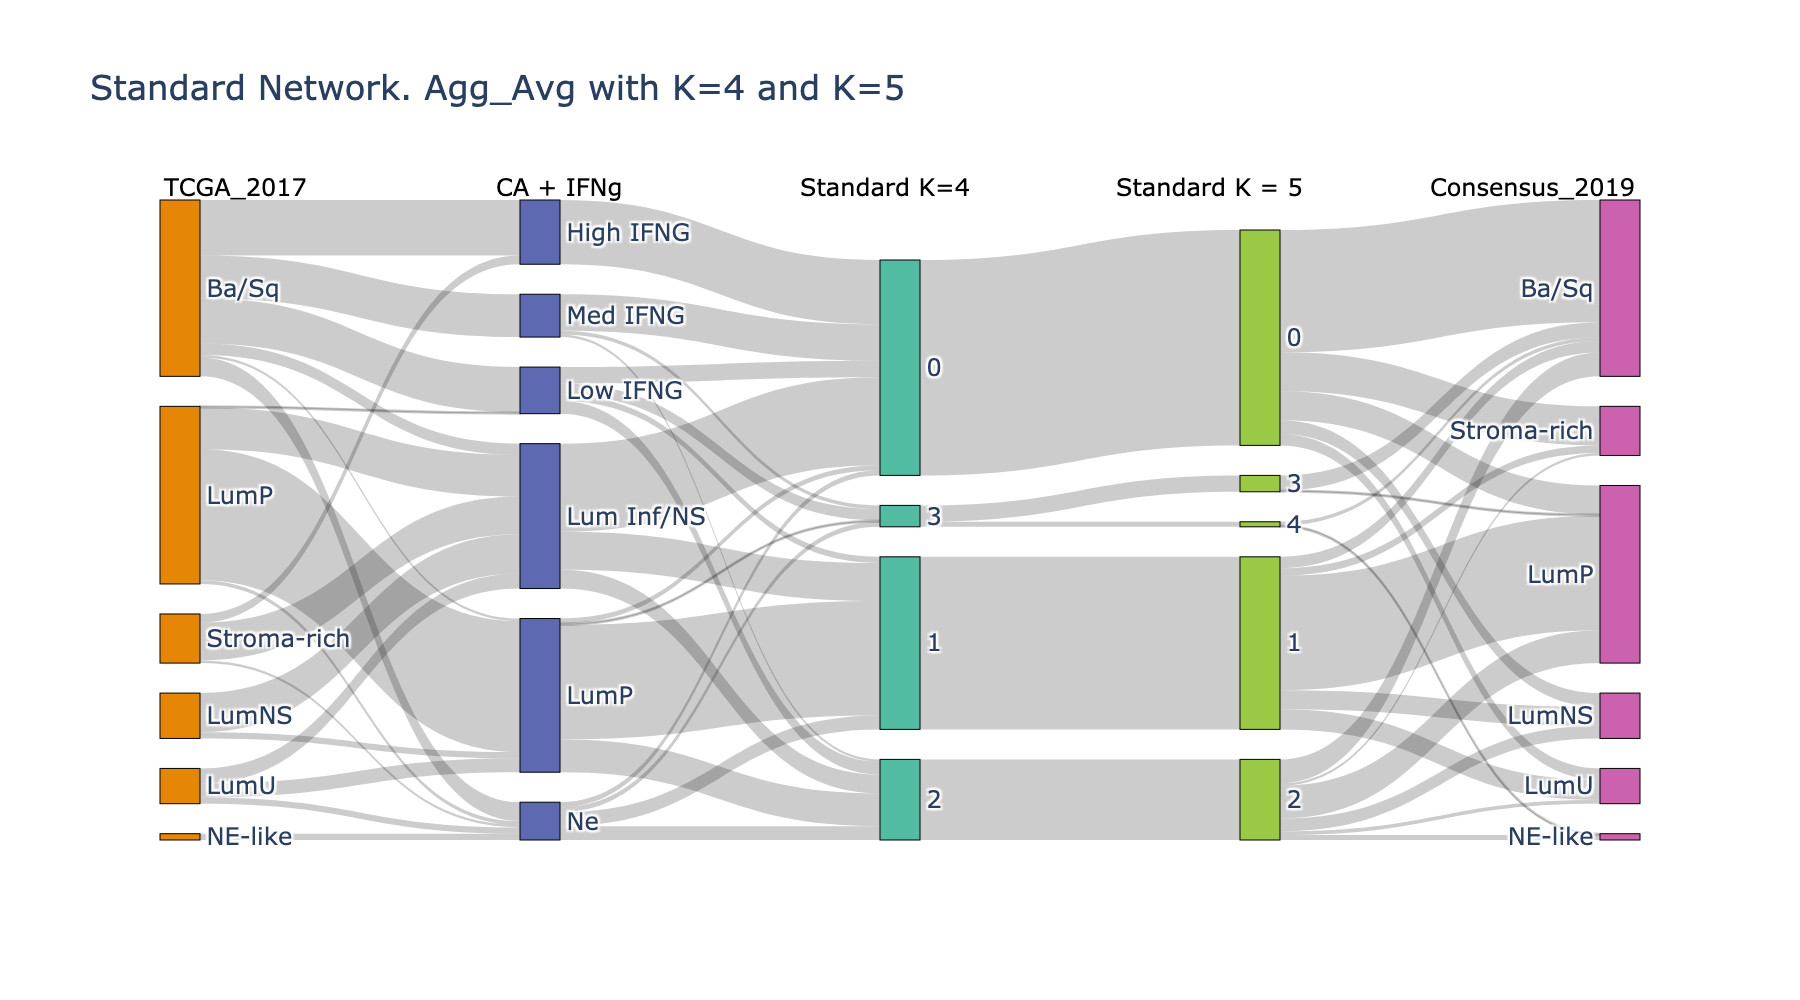
\includegraphics[width=\textwidth,keepaspectratio]{Sections/Network_I/Resources/P0/Sankey_Avg_4K.png}
        \caption{Agglomerative with average linkage}
    \end{subfigure}
    \hfill
    \caption{Sankey plots for the two best performing models. }
    \label{fig:N_I:p0_sky_Agg_KMeans}
\end{figure}


Two Sankey plots in Figure \ref{fig:N_I:p0_sky_Agg_KMeans} are used to assess the differences in the MIBC subtyping between the two best clustering model and the two cluster sizes\footnote{The standard networks were only used for comparison to simplify the process.}. There is a striking difference between the two clustering models, Agg\_Avg finds disproportionate clusters while the K-means finds similar size groups. This, together with the High IFNG subgroup found by K-means suggests that this model is the best choice. 


The cluster metrics are not very useful in determining the number of clusters, the scores decrease proportionally with the number of clusters, thus the best result if given by the lowest K. Elbow method helps in this case but one it is a heuristic approach. In Figure \ref{fig:N_I:p0_sky_Agg_KMeans} A) when K=5, the larger group 0 from K=4 is split into smaller groups, see subtype 2 \& 5 (when K=5). For this and the fact that it is expected to find larger groups K=5 is preferred over K=4.


\subsubsection{Network comparison}


Figure \ref{fig:N_I:p0_sky_leiden} represents an overview of the decisions made in the previous sub-sections, K-means (K=5) was found to be the most suitable clustering model. The three networks are compared with the consensus and TCGA classifiers \citet{Kamoun2020-tj, Robertson2017-mg} as well as our subtyping from Section \ref{}). From the top left figure it can be observed that there number of communities is similar across the three networks, there are 9 or 10 with a few exceptions. There are significantly less communities compared with the number of subgraphs found in the tumour network; see Figure \ref{fig:N_I:tum_leiden_modifiers}. The small variance of the Modularity score in the Figure on the right suggests that the communities are fairly stable and the penalised network have a lower performance by 0.04.

\begin{figure}[!htb]    
    \centering
    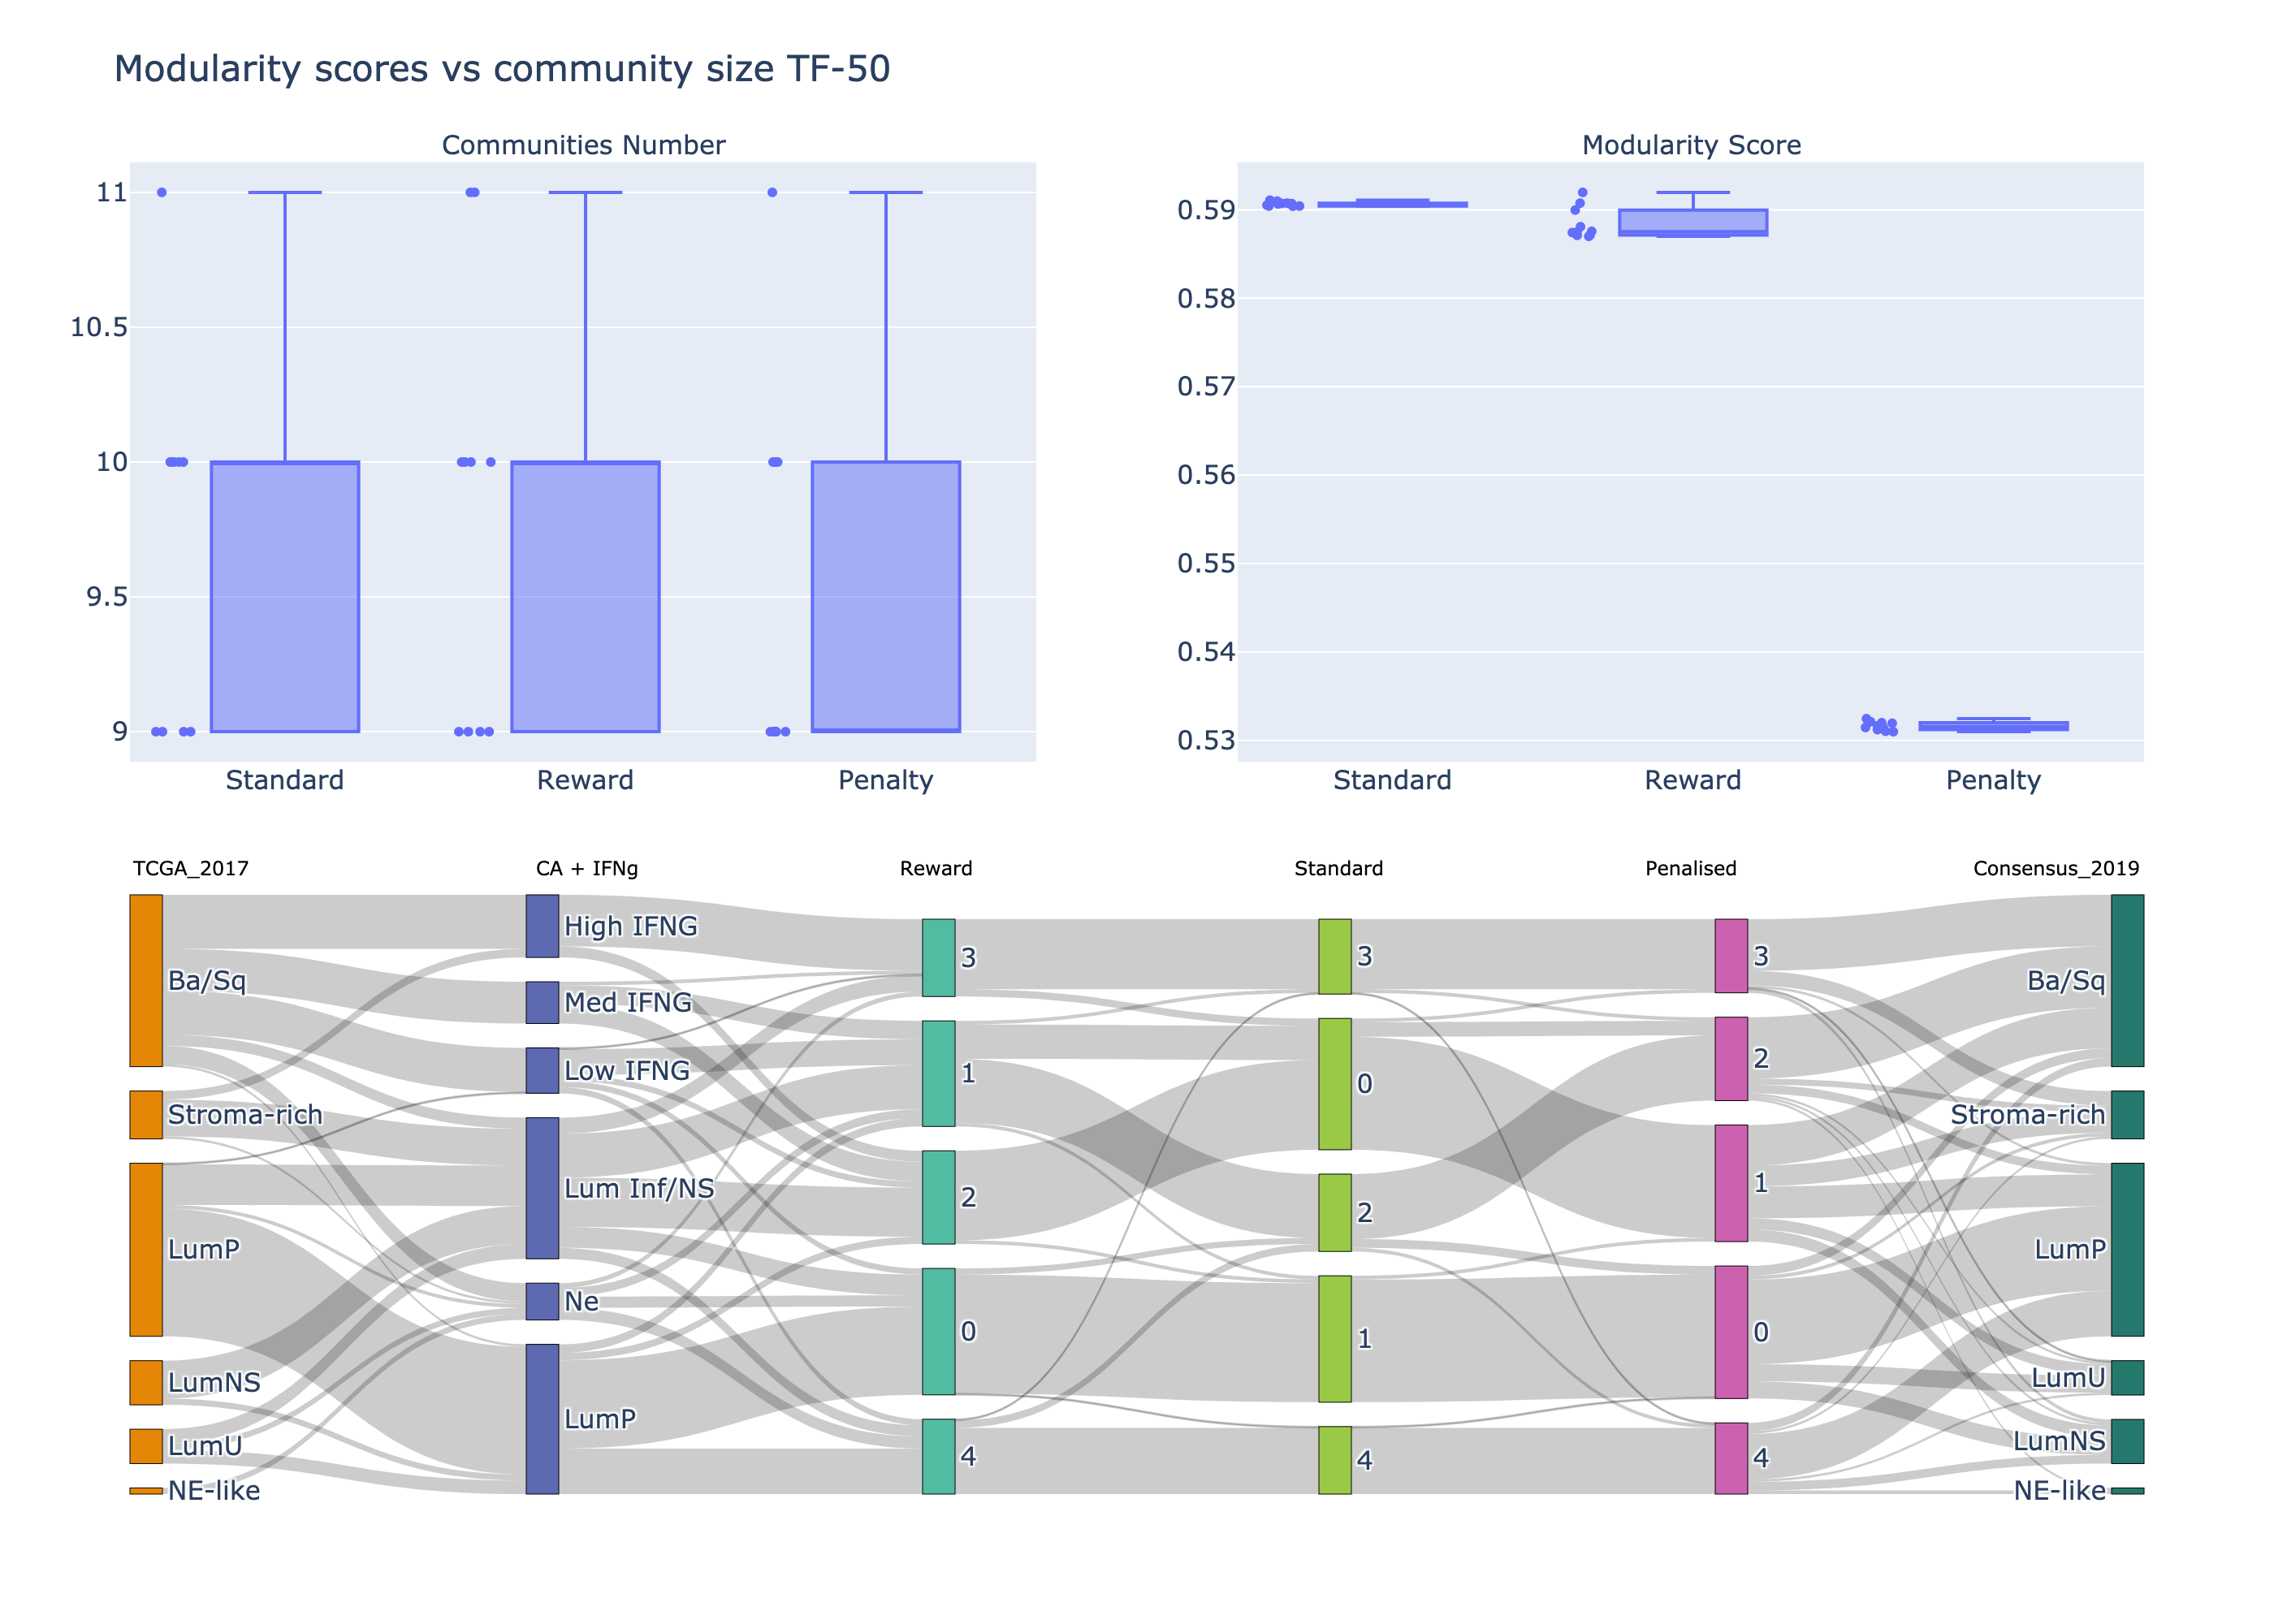
\includegraphics[width=1.0\textwidth,height=0.7\textheight,keepaspectratio]{Sections/Network_I/Resources/P0/Ldn_Sky_TF_50_RawKMeans_K5.png}
    \caption{Overview of the MIBC stratification using P0 dataset.}
    \label{fig:N_I:p0_sky_leiden}
\end{figure}

From the Sankey plot it can be seen that the High IFNG group (CA+IFNg) is contained across the 3 networks in cluster 3. Groups 2 in Standard and Penalised are similar and formed mostly from Ba/Sq groups while cluster 1 (Reward) has additional samples from LumInf/NS\footnote{Would this mean that by increasing the weight values more samples are added to the group? While pruning edges removes some of the noise?}. The cluster 0 from the Standard network resembles to the LumInf/NS group from the CA+IFNG classification, being a mixed of samples. Group 0 (Reward and Penalised) and 1 (Standard) contains samples which previously were considered Luminal samples. Lastly, cluster 4 contains a consistent number of samples which previously classified as LumP or/and Luminal Unstable (LumU), Unspecified (LumNS).

Overall, the comparison between classifications shows that the network approaches exhibit different subtypes from the other traditional methods. Several samples change group membership in the three different networks, but there are no large changes. This suggests that the weight modifiers strategies have little effect on the subtyping.


\subsubsection{Community analysis}


\begin{figure}[!htb]
    \hfill
    \begin{subfigure}[b]{0.49\textwidth}
        \centering
        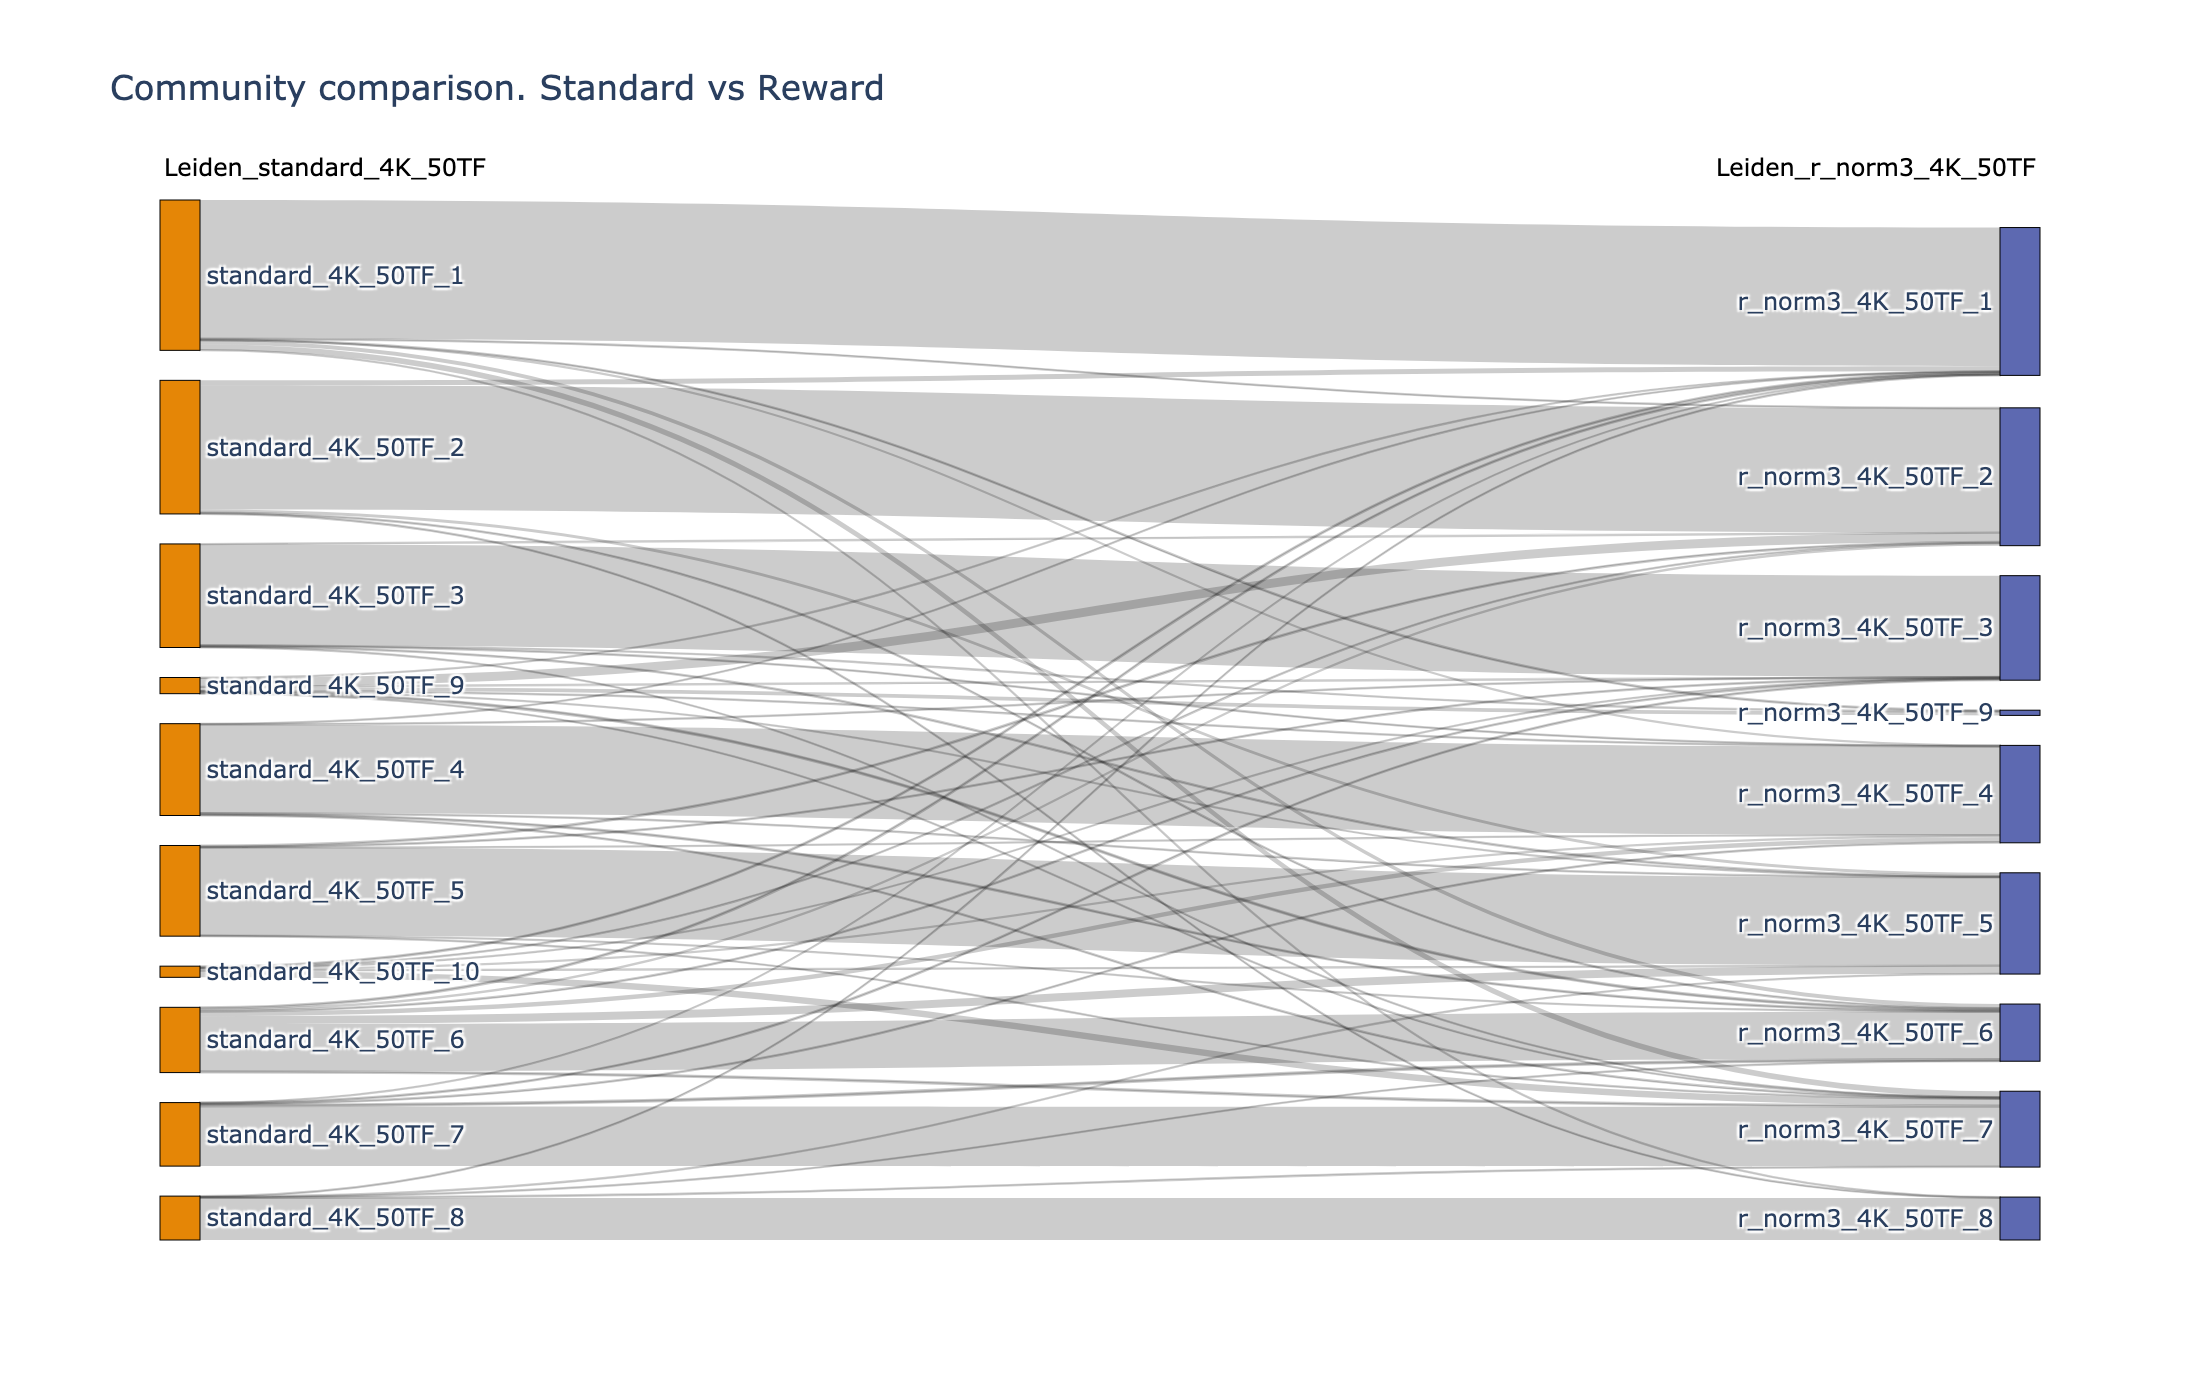
\includegraphics[width=\textwidth,keepaspectratio]{Sections/Network_I/Resources/P0/Comms/Sky_Comm_Comp_4K.png}
        \caption{Gene changes}
    \end{subfigure}
    \hfill
     \begin{subfigure}[b]{0.49\textwidth}
            \centering
            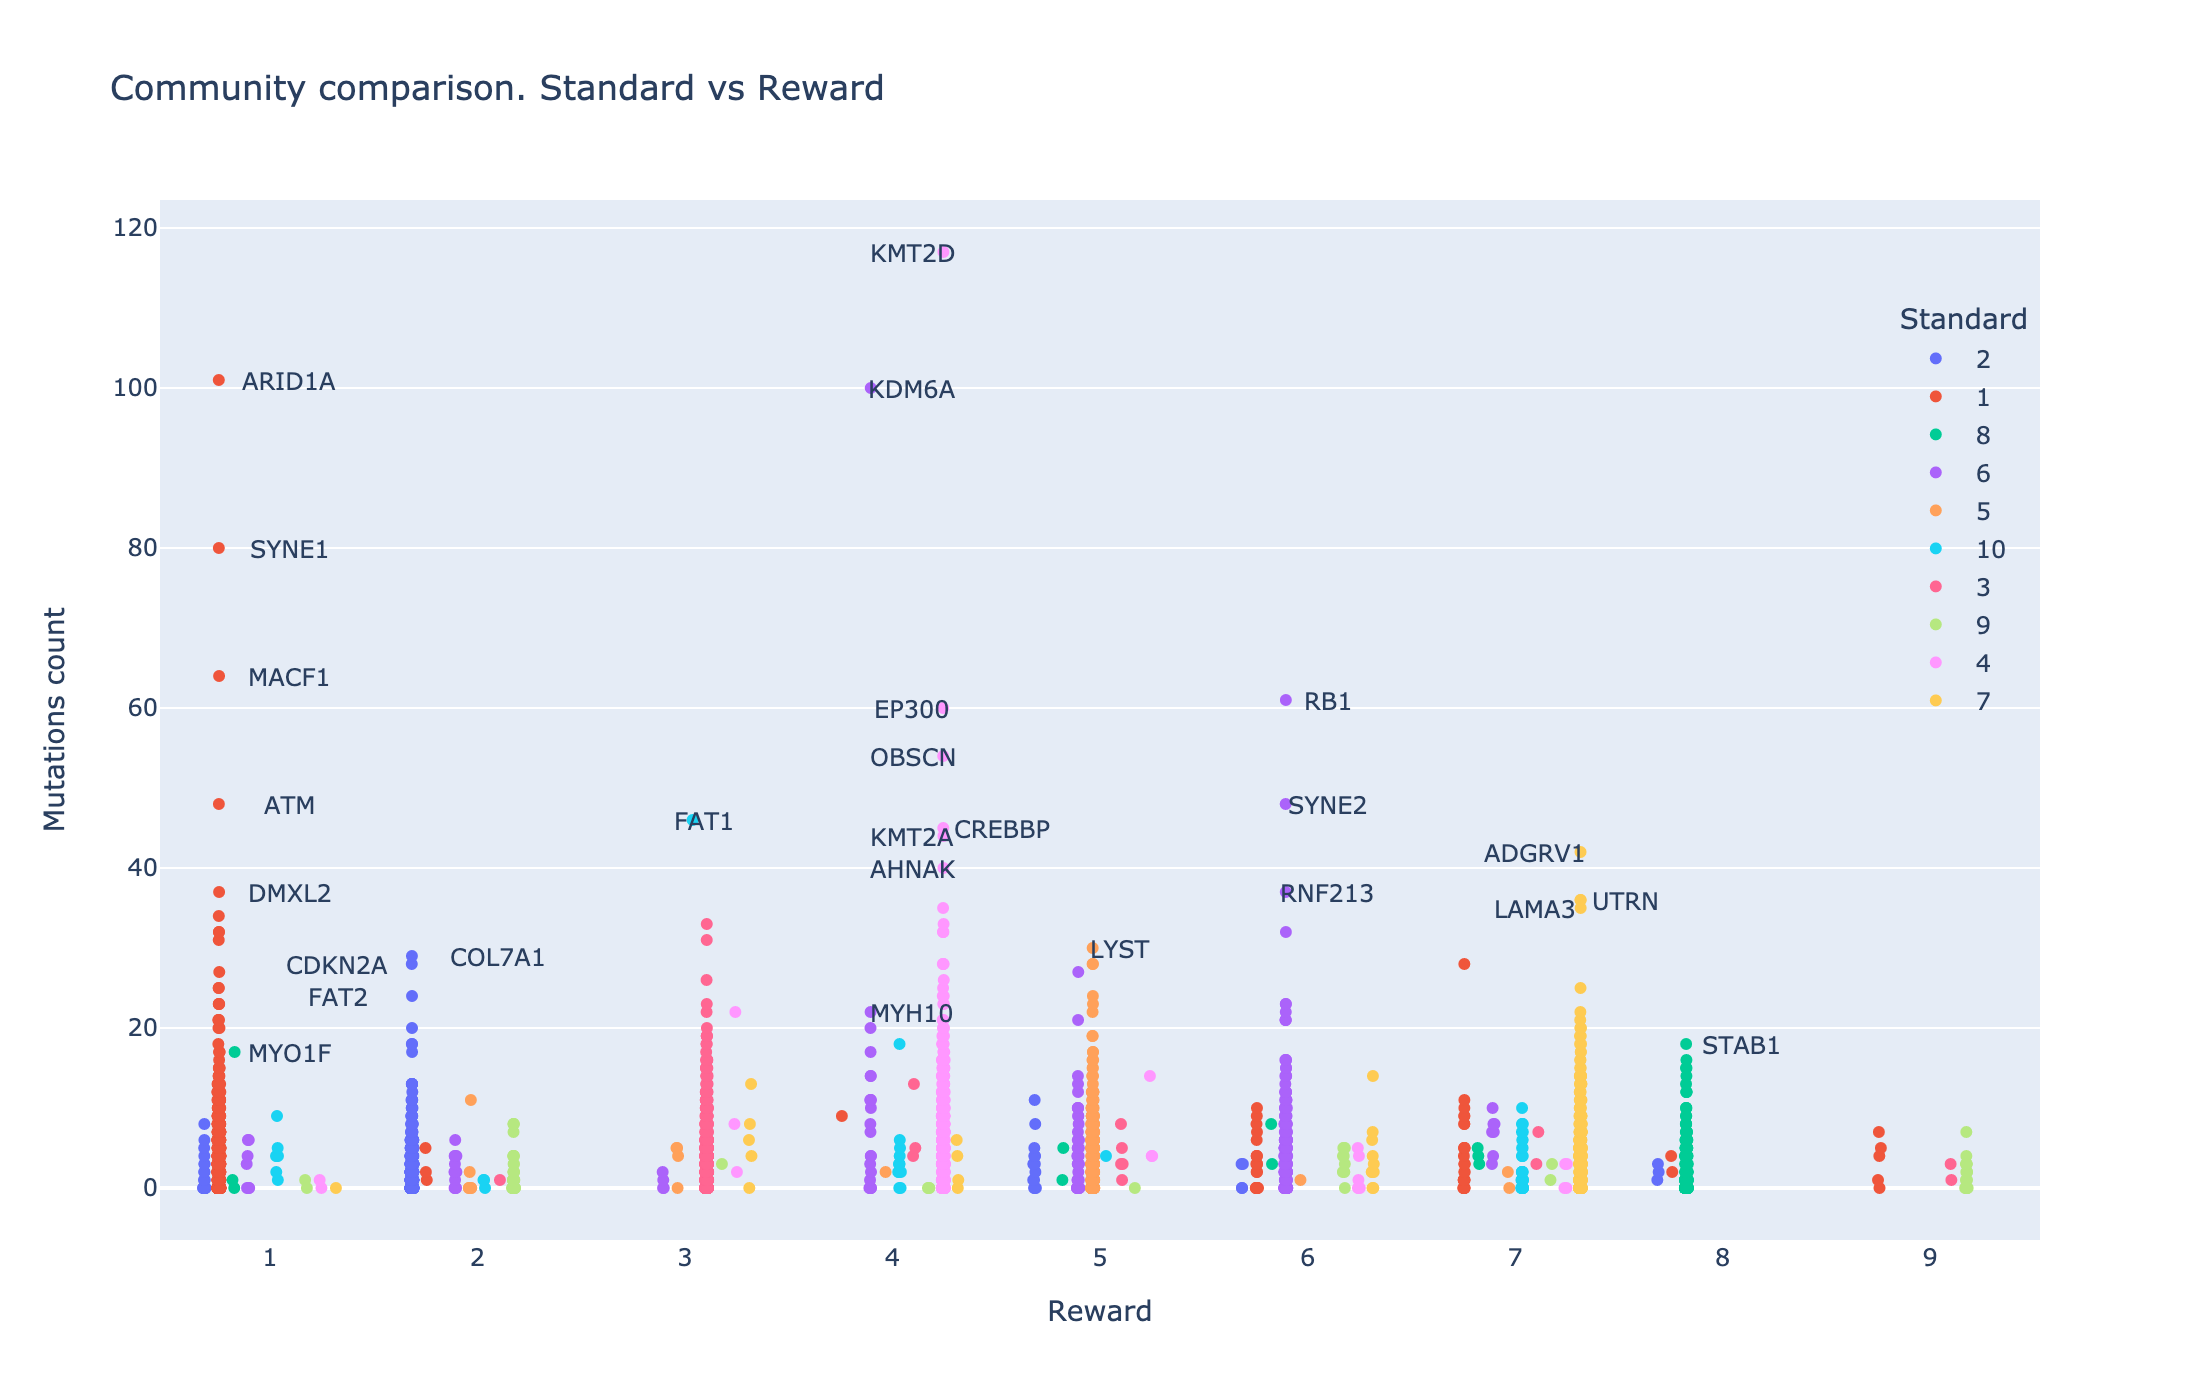
\includegraphics[width=\textwidth,keepaspectratio]{Sections/Network_I/Resources/P0/Comms/Mut_Comm_Comp_4K.png}
            \caption{Mutation representation}
    \end{subfigure}
    \hfill
    \hfill
    \begin{subfigure}[b]{0.47\textwidth}
        \centering
        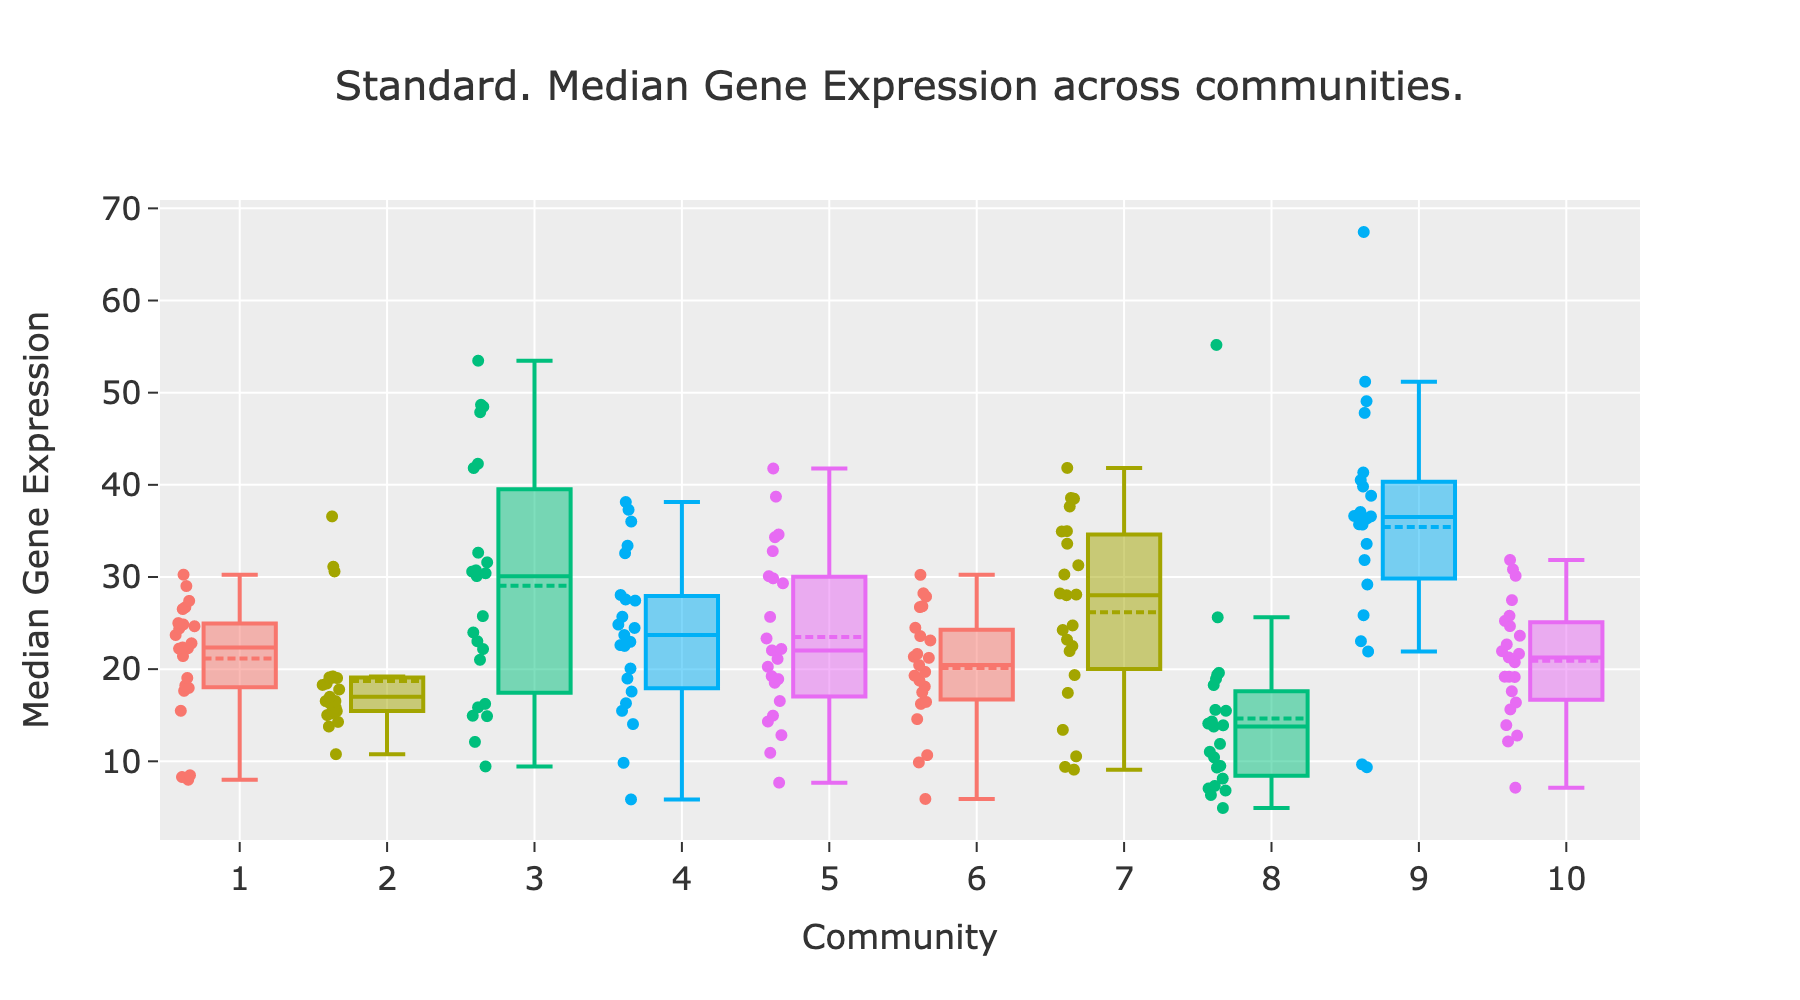
\includegraphics[width=\textwidth,keepaspectratio]{Sections/Network_I/Resources/P0/Comms/P0_standard_4K_50TF_med.png}
        \caption{Standard expression values}
    \end{subfigure}
    \hfill
    \begin{subfigure}[b]{0.47\textwidth}
        \centering
        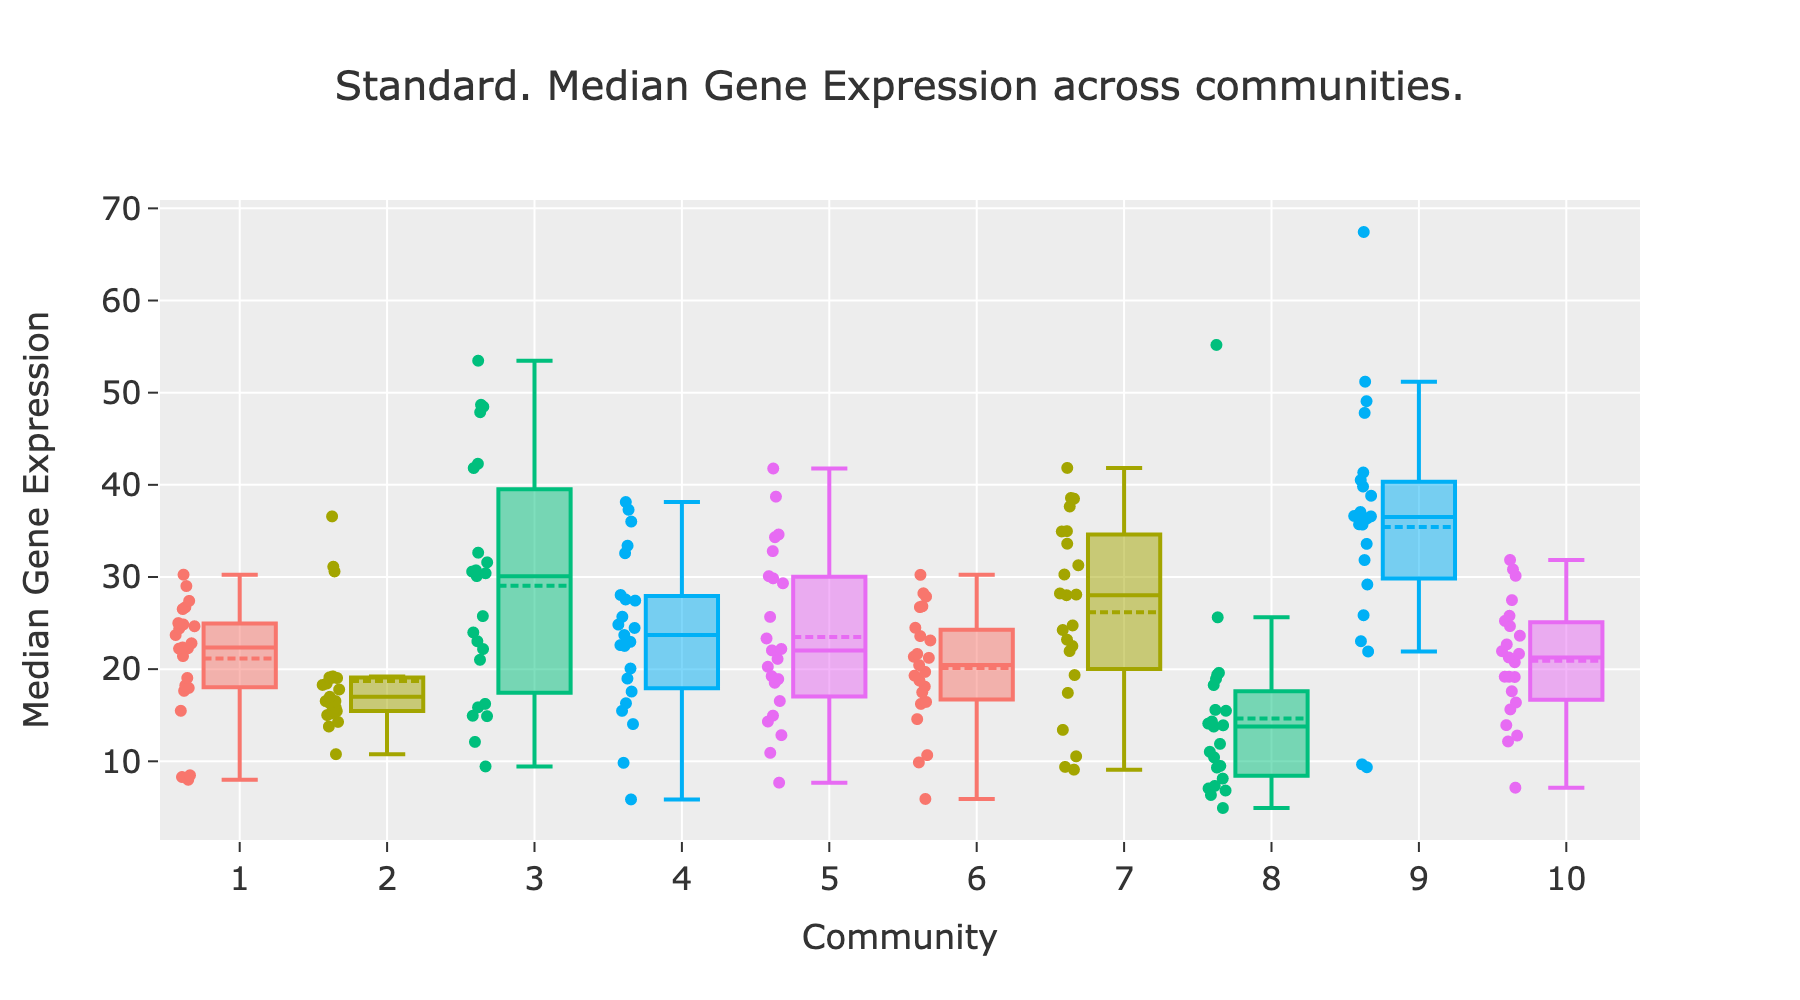
\includegraphics[width=\textwidth,keepaspectratio]{Sections/Network_I/Resources/P0/Comms/P0_standard_4K_50TF_med.png}
        \caption{Reward expression values}
    \end{subfigure}
    \hfill
    \caption{Gene communities changes.}
    \label{fig:N_I:p0_comm_chgs}
\end{figure}




\begin{figure}[!htb]
    \hfill
    \begin{subfigure}[b]{0.49\textwidth}
        \centering
        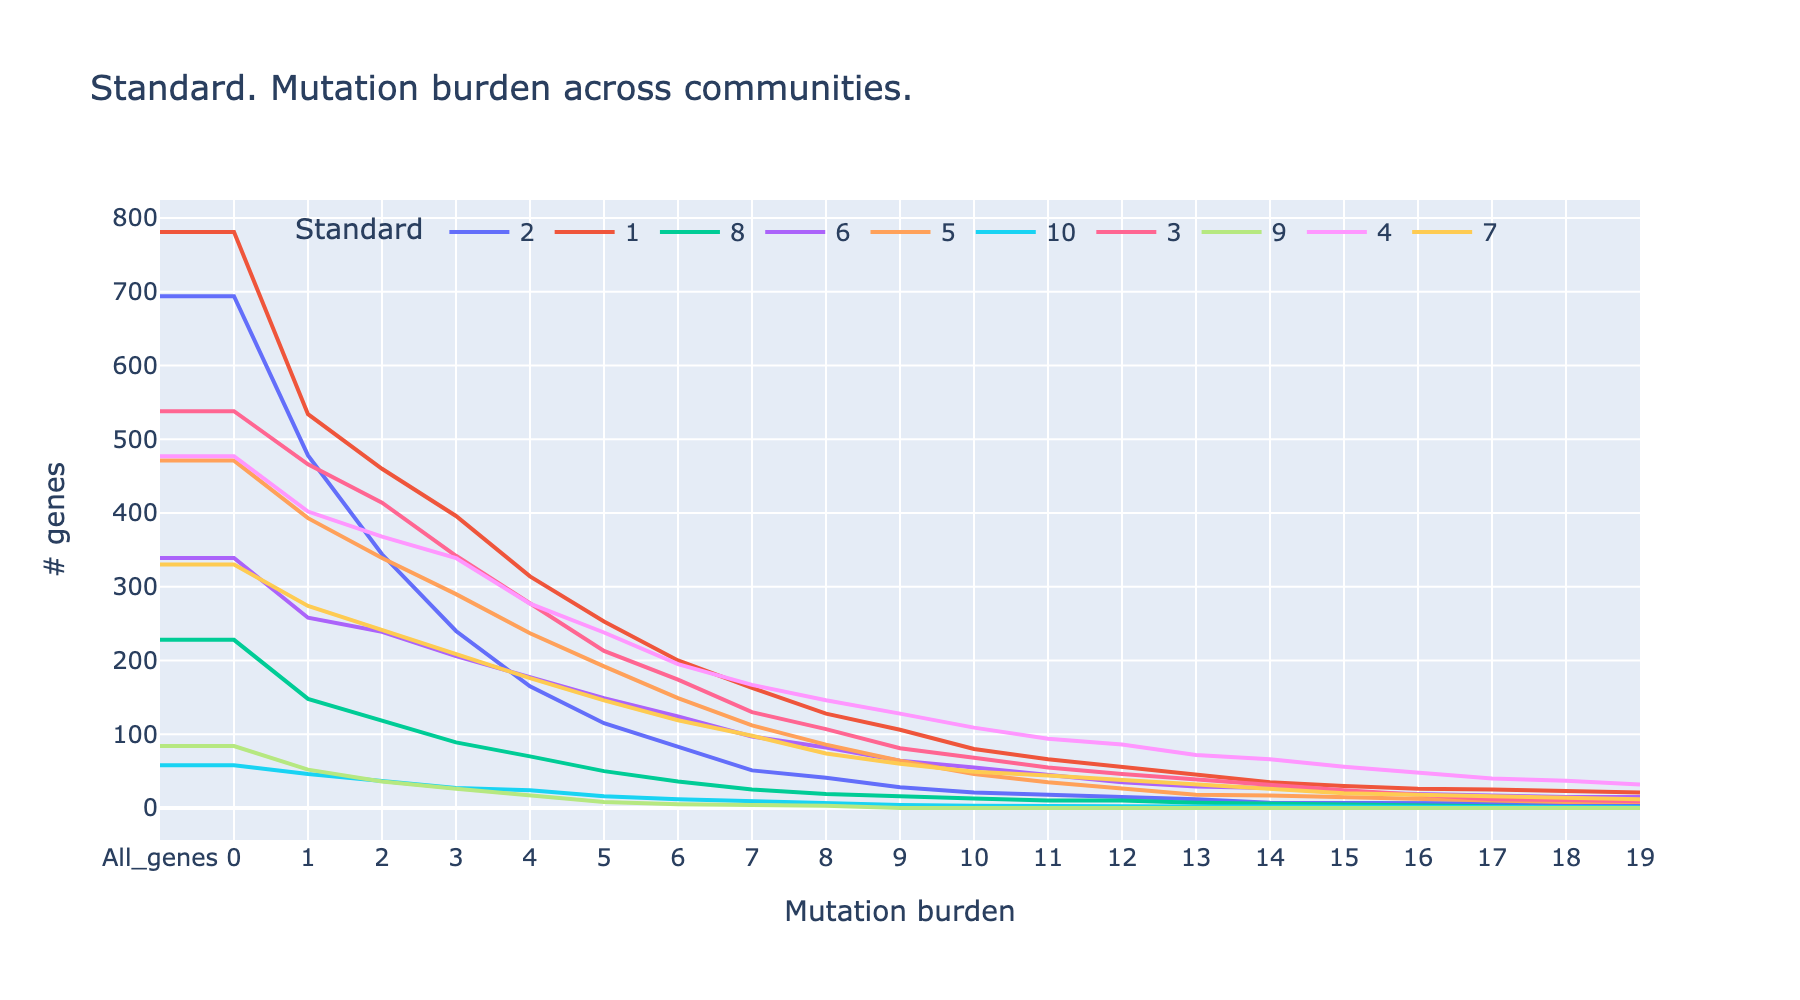
\includegraphics[width=\textwidth,keepaspectratio]{Sections/Network_I/Resources/P0/Comms/Mut_evo_Std_4k.png}
        \caption{Standard}
    \end{subfigure}
    \begin{subfigure}[b]{0.49\textwidth}
        \centering
        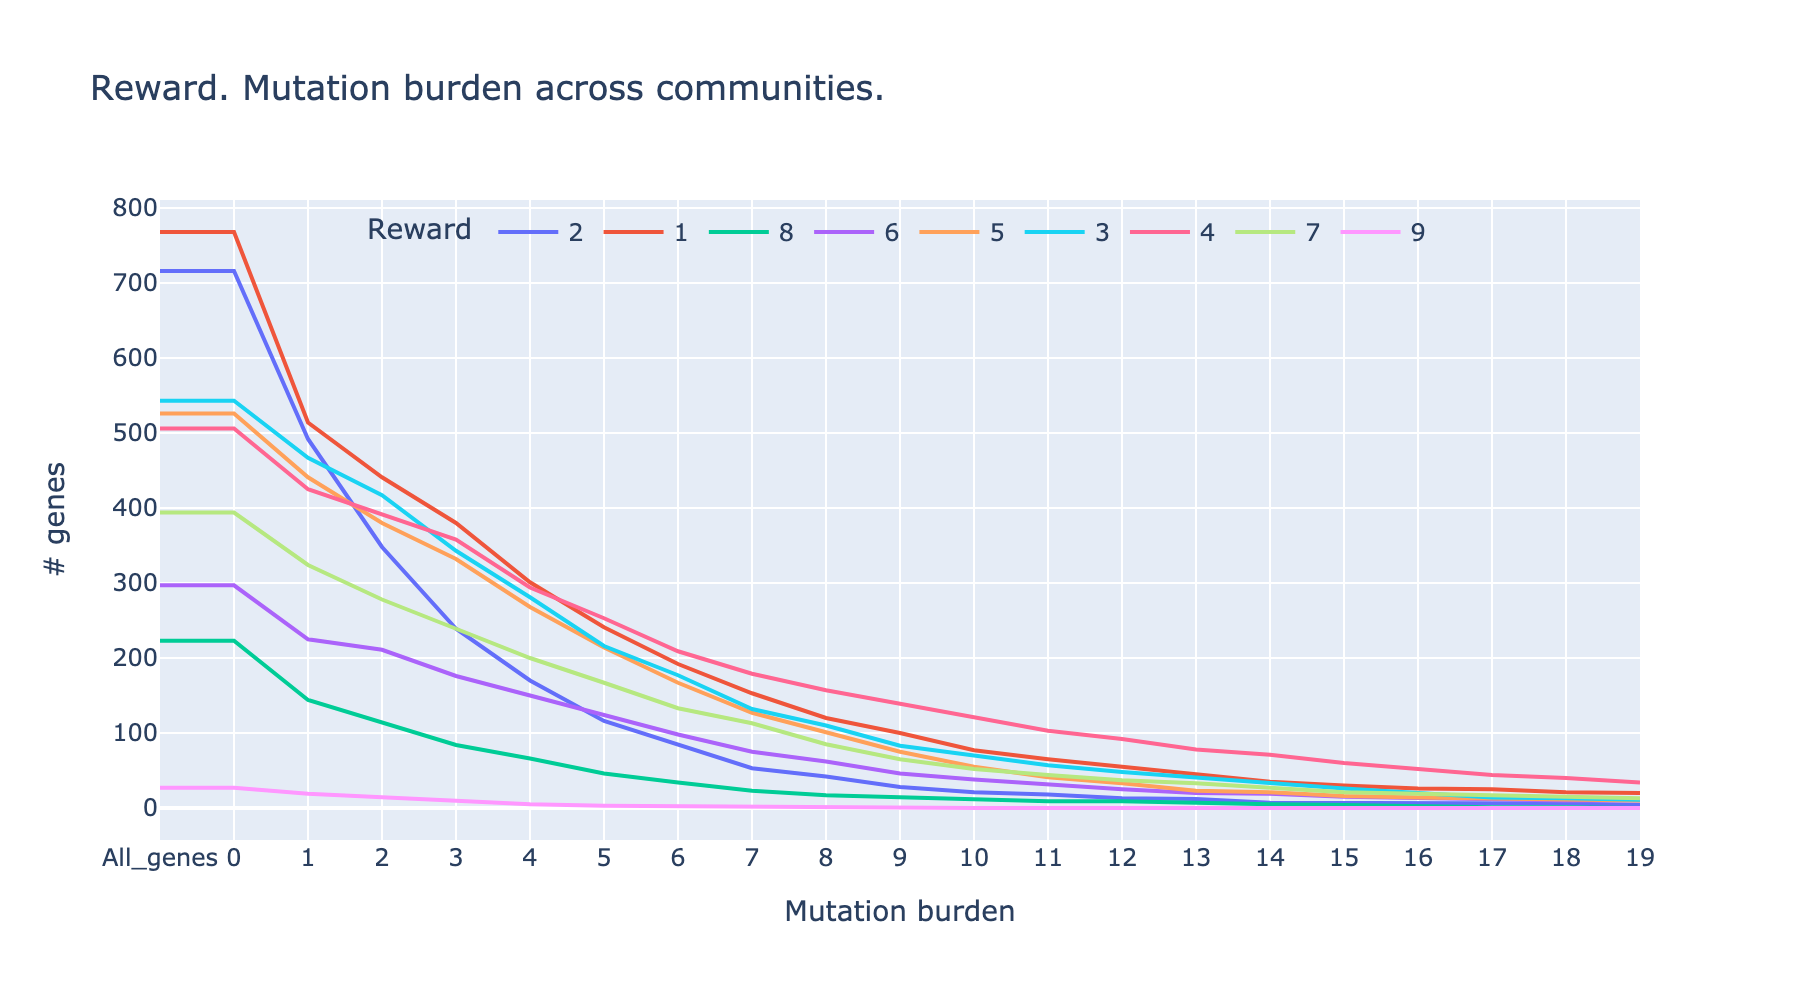
\includegraphics[width=\textwidth,keepaspectratio]{Sections/Network_I/Resources/P0/Comms/Mut_evo_Rwd_4k.png}
        \caption{Reward}
    \end{subfigure}
    \caption{Mutation burder per communities}
    \label{fig:N_I:p0_mut_burden}
\end{figure}



To understand the lack of changes



\newpage

\begin{figure}[!htb]
    \hfill
    \begin{subfigure}[b]{0.47\textwidth}
        \centering
        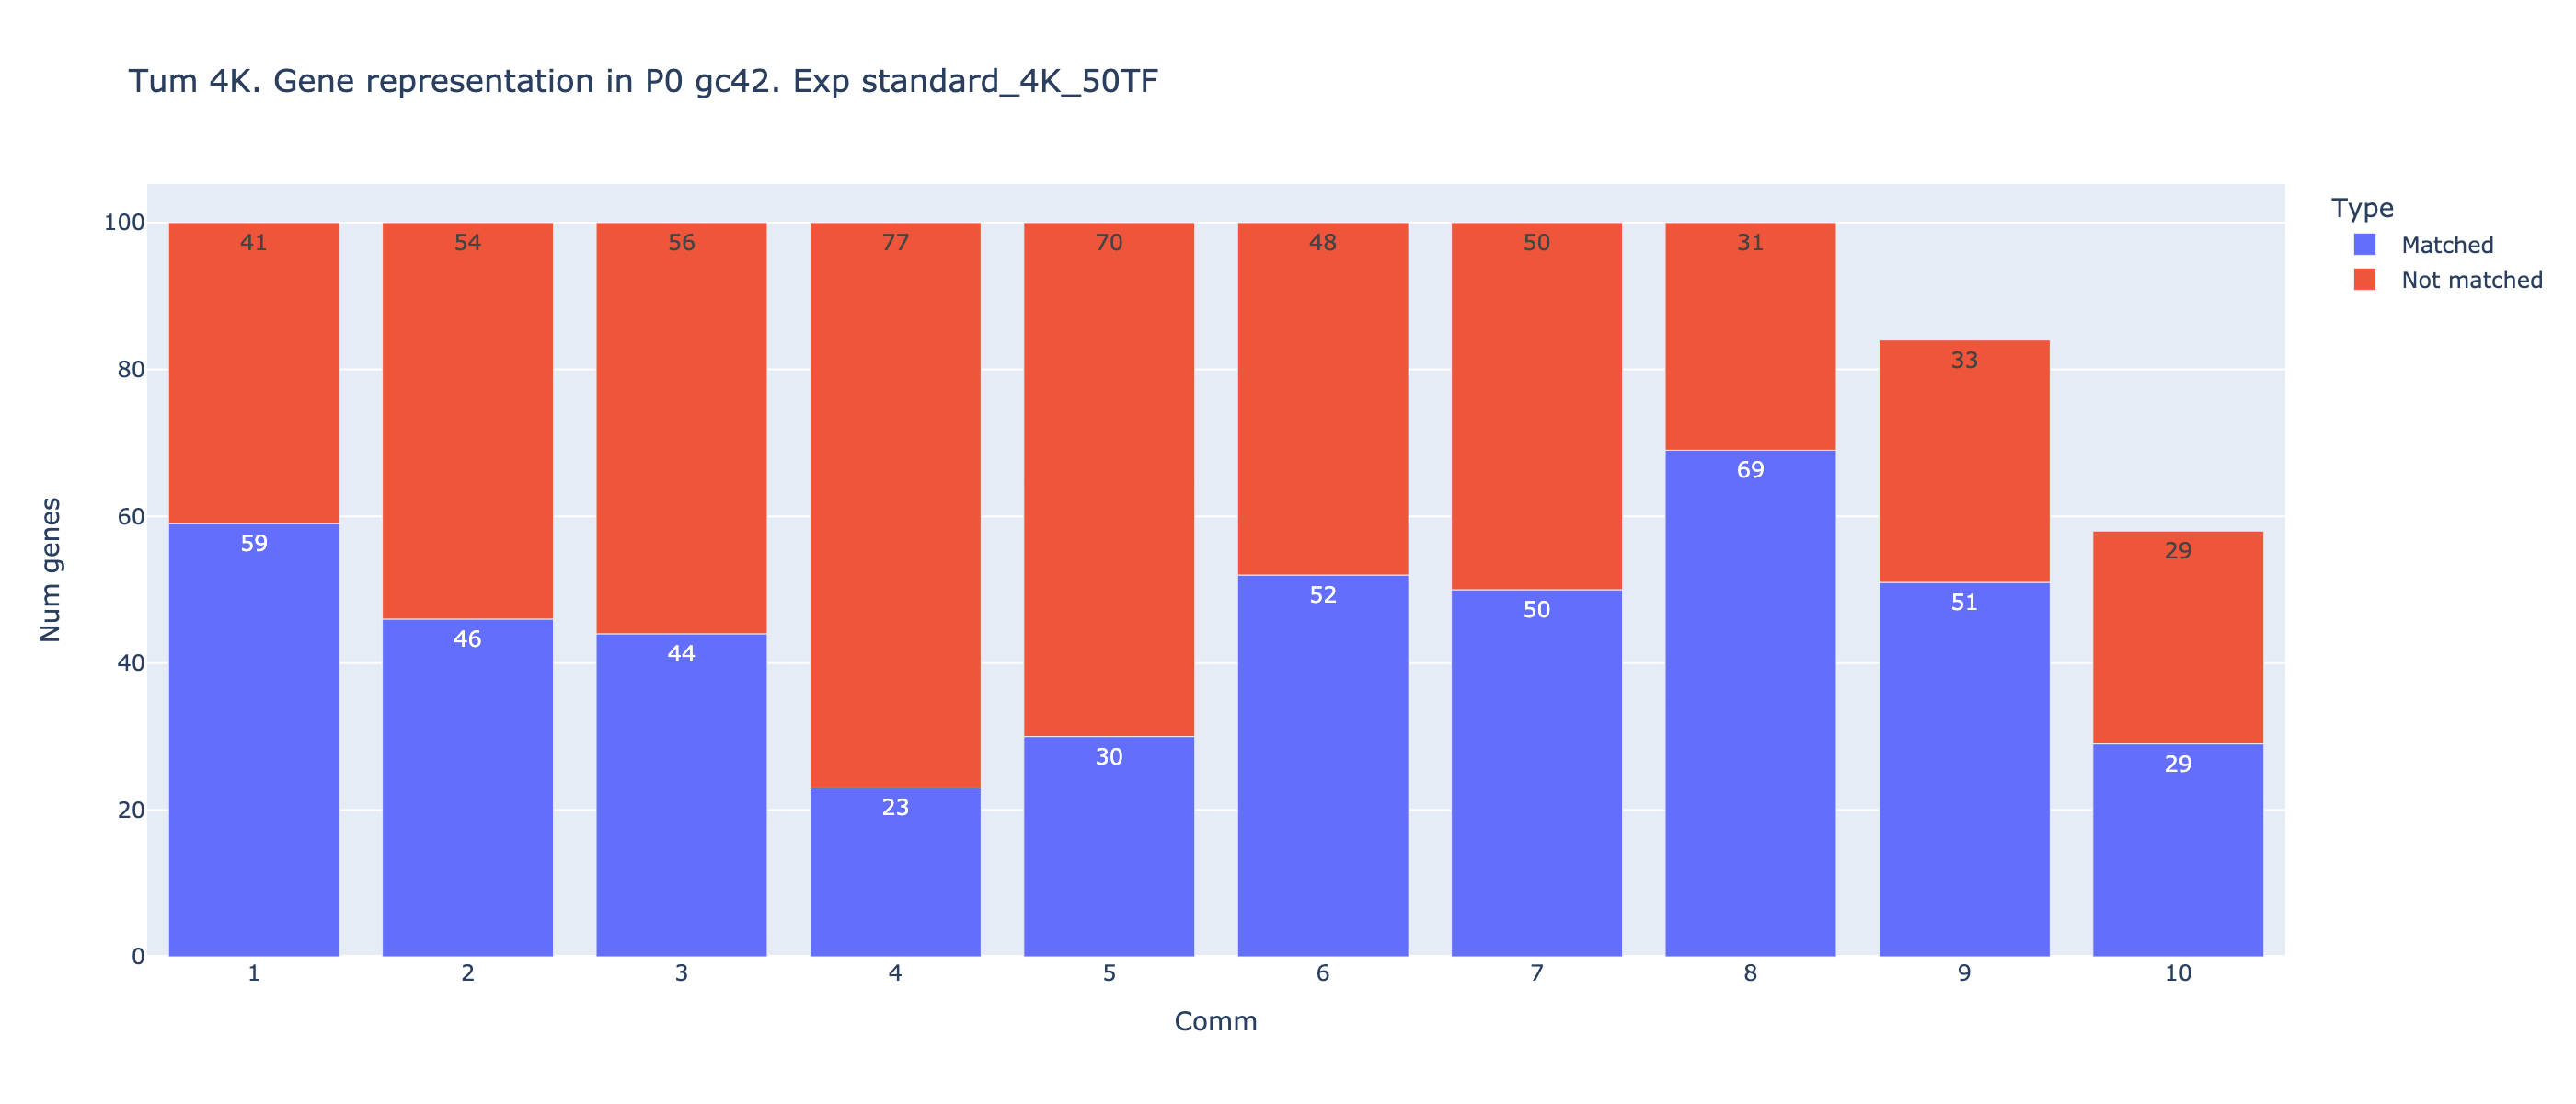
\includegraphics[width=\textwidth,keepaspectratio]{Sections/Network_I/Resources/P0/4K_p0_modConMev_rep_standard_4K_50TF.png}
        \caption{The most relative varied genes}
    \end{subfigure}
    \hfill
    \begin{subfigure}[b]{0.47\textwidth}
        \centering
        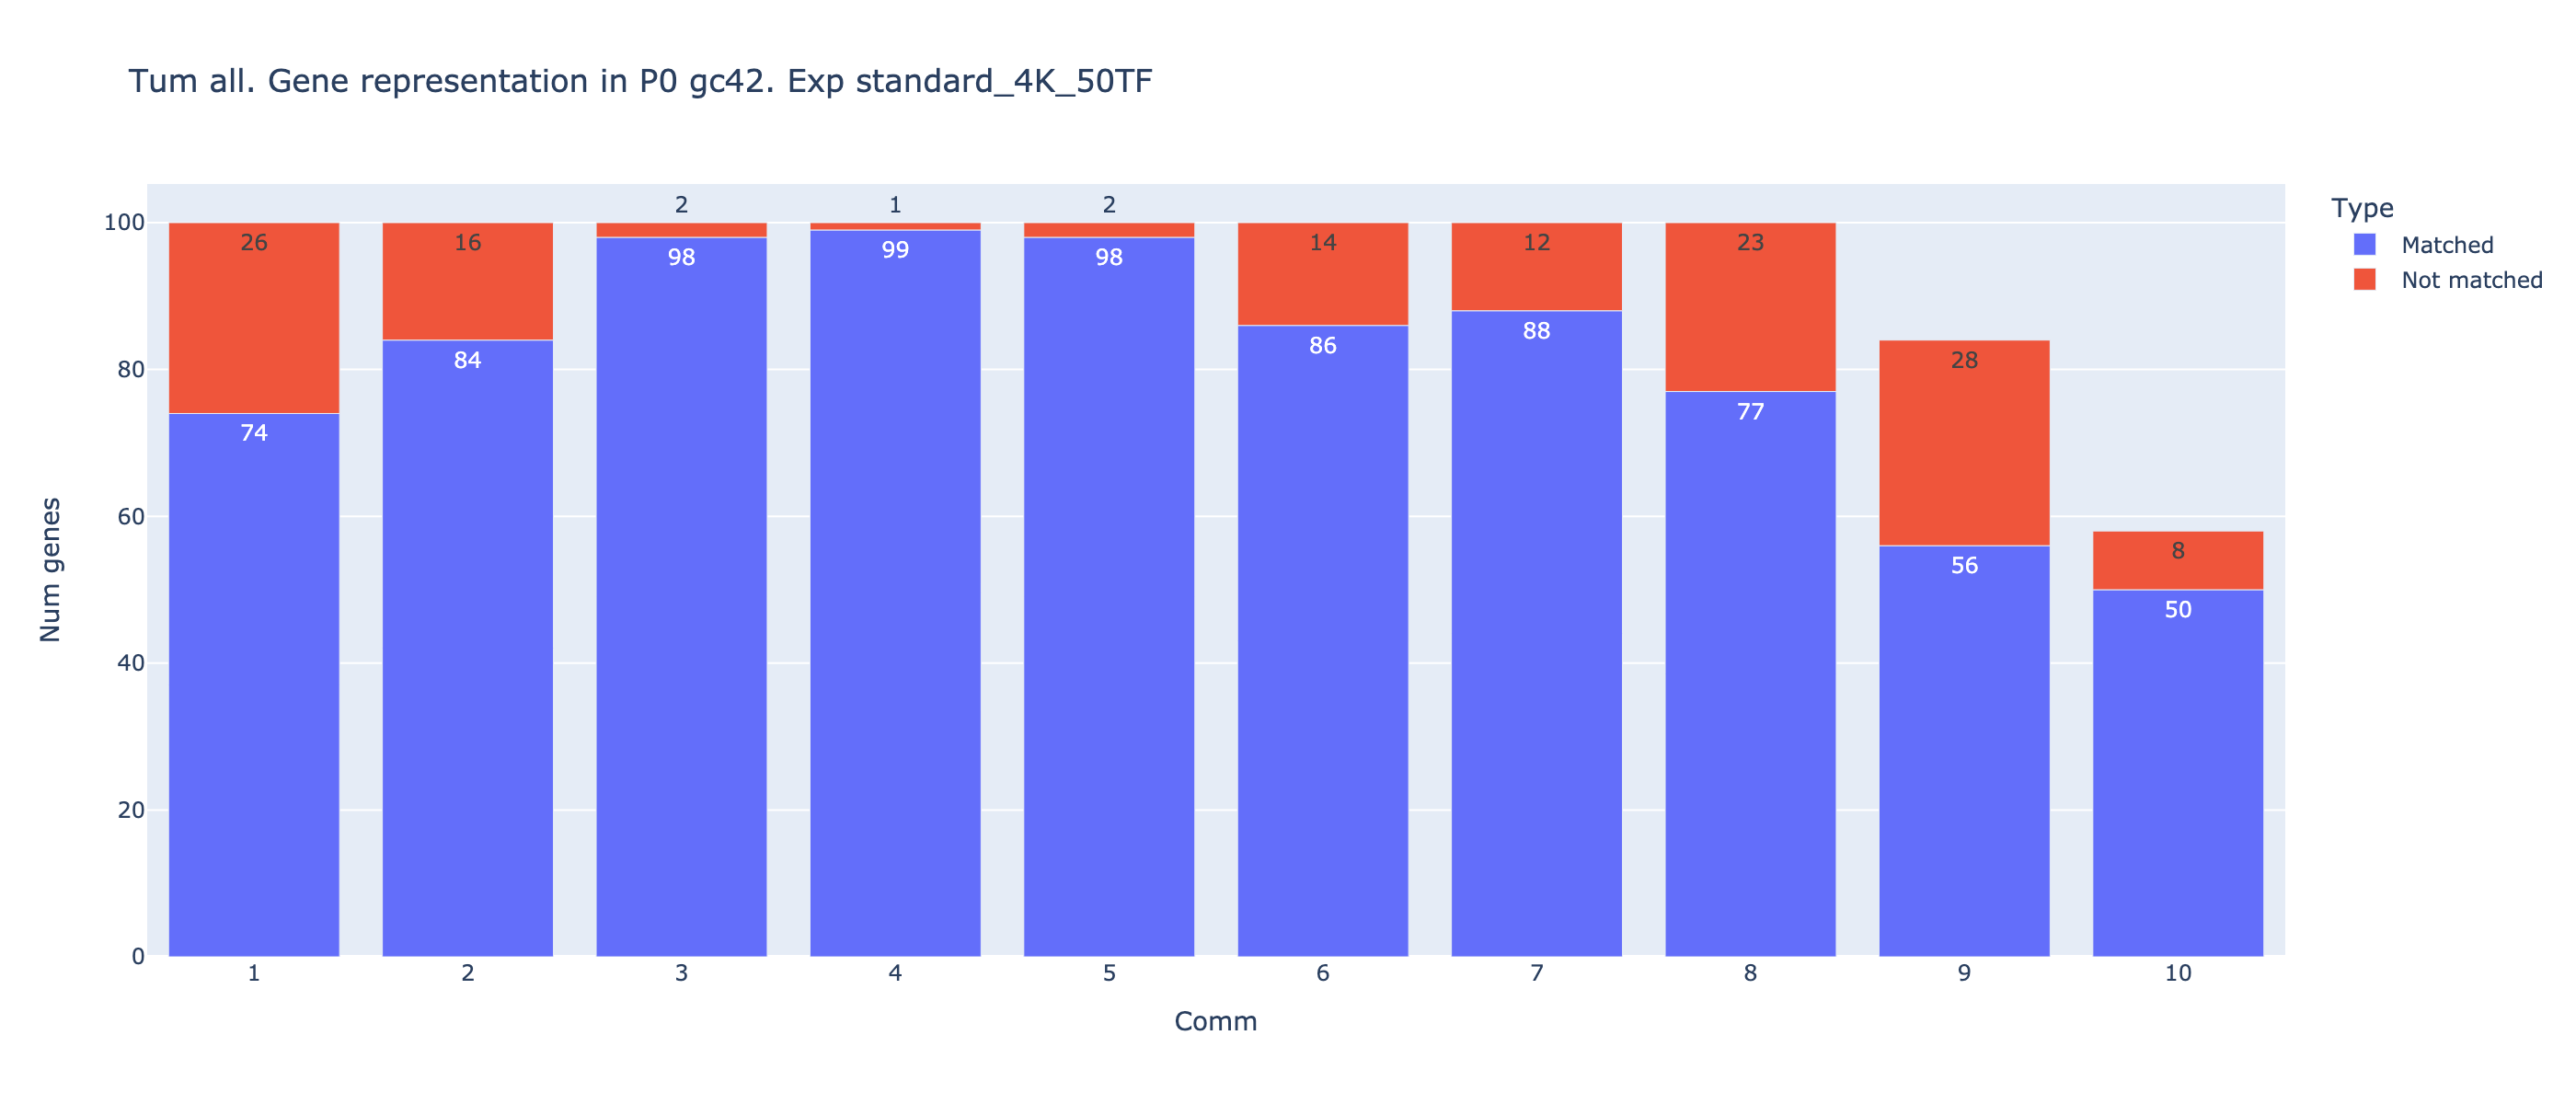
\includegraphics[width=\textwidth,keepaspectratio]{Sections/Network_I/Resources/P0/10K_p0_modConMev_rep_standard_4K_50TF.png}
        \caption{All the genes expressed}
    \end{subfigure}
    \hfill
    \caption{Genes found in the tumour dataset for each network community. The top 100 genes are selected by ModCon score. A) Is when the tumour dataset is restricted to the top most varied genes B) Includes all the expressed genes in the tumour dataset. }
    \label{fig:N_I:p0_mev_rep}
\end{figure}



\newpage

% Reason 1 for why this approach is not good - poor gene representation in the tumour
In the first experiment run, with 4K genes I have noticed that there were not that many changes between communities when the modifier is applied. This is different from what I intended to see when modifiers are applied. We want to see better separation between communities, with smaller and more dedicated biological processes. Thus, I have started investigating this during which I found out that there is a poor representation of the genes mutated in the P0 samples. Thus lead to further investigating on how to select the genes for the PGCNA; this was covered in this section \ref{Sec:N_I:gene_sel}.

To support this argument the following figures are needed:
\begin{itemize}
    \item Sankey plot with the community changes
    \item Bar Figure to show the mutation representation in each community in the P0 dataset. Figure \ref{fig:N_I:P0_median}
    \item Show the mutation intensity (i.e. mutation count) evolution when applying different threshold.  Figure \ref{fig:N_I:P0_comp}
    \item The median gene expression of the genes in each community. See Figure \ref{fig:N_I:P0_comp}.
    \item Experiments with 10K and that there is too much noise. The reason for doing this is that I wanted to have more genes from the P0 included in the Tumour dataset
\end{itemize}

% Reason 2 - Scatter biological pathways 
Further on, when we look at the biology of each community we could see that there a lot shared pathways across communities. This include PDGF, CCKR, apoptosis and others. This gives the impression that the approach developed did the contrary from the intended behaviour, instead of isolating the biological processes it scattered through the network. The pathways were discovered through the Gene Ontology tool using PANTHER Pathway option and \textbf{no correction}; the latter because the majority of the genes inputted were \textbf{not} given significant results. This further strengthen our intuition that this approach is not providing the intended results.

Figures I need to support for the above argument:
\begin{itemize}
    \item Pick 2-3 pathways from the ones found and highlight in the network.
    \item Maybe put the Network with annotations?
\end{itemize}

% Reason 3 - Effect of the TF. but this really is 
While performing the biological interpretation, looking at the genes selected by ModCon score, it can be clearly noticed that the TF genes play a major role in the networks. The reason for this is that in this set of experiment we enable 50 edges for each Transcription Factor, thus biasing the network for these genes. Definitely, this parameter have a large impact of ModCon. Therfore, we performed an experiment with a lower number of edges per TF and we found out that there are more communities with fewer communties.
Figure supporting the above:
\begin{itemize}
    \item How many of the genes selected from the ModCon are a TF? Give some stats
    \item The sub-graph where only the ModCon genes are selected for each community; with the size of the TF \ref{fig:N_1:tf_comp}
\end{itemize}

% Reason 4 - Linking to the tumour stratification 
An open problem to the network selection process is how to link back the genes used in a healthy network to tumour stratification. When tried to apply MEV on the genes selected with the P0 + mutations-count there weren't that well represented in the TCGA's dataset with the same number of genes (4K) - ~1/3 of the genes were presented. However, when all the (basic filtered) 13k genes from the tumour dataset were used, there was a better match. Also, when comparing with the other cohorts didn't make sense, the Basal split wasn't present in neither of the networks. Regardless of the representation, this approach is not fulfilling the initial task which is to integrated the tumour and healthy as it stratifies just by the GE from P0 and doesn't consider the GE from tumour dataset.
To support this argument the following figures are needed:
\begin{itemize}
    \item Stats showing the representation of the selected genes through P0 in the TCGA data
    \item A Morpheus plot with the hierarchical clustering for the one of the P0 experiments
    \item Sankey plot of the Tumour stratification when the genes selected with the P0.
\end{itemize}


\subsubsection{Conclusion}

There are a few argument made against this experiment:
\begin{itemize}
    \item The number of connections a gene has a similar effect to the reward modifier. (thinking of the Sankey plot when TF=10 and std-norm3 on P0). This is somehow expected as in the PGCNA paper the author says that more connections yield less communities.
    \item P0 dataset may not have enough power to form smaller communities. This would be verified in the next experiments with TF=10
    \item Many genes from the P0 selection network are missed in the TCGA and the GE of the tumour are not considered.
    \item There is a bias in the gene selection, when the most varied are used, and sometimes the one with the highest magnitude are omitted. Thus experiments to include genes with highest variance, magnitude and mutation count
\end{itemize}


\subsubsection{Draft Figures}

\begin{figure}[H]
    \captionsetup[subfigure]{justification=Centering}
    \begin{subfigure}[t]{0.5\textwidth}
        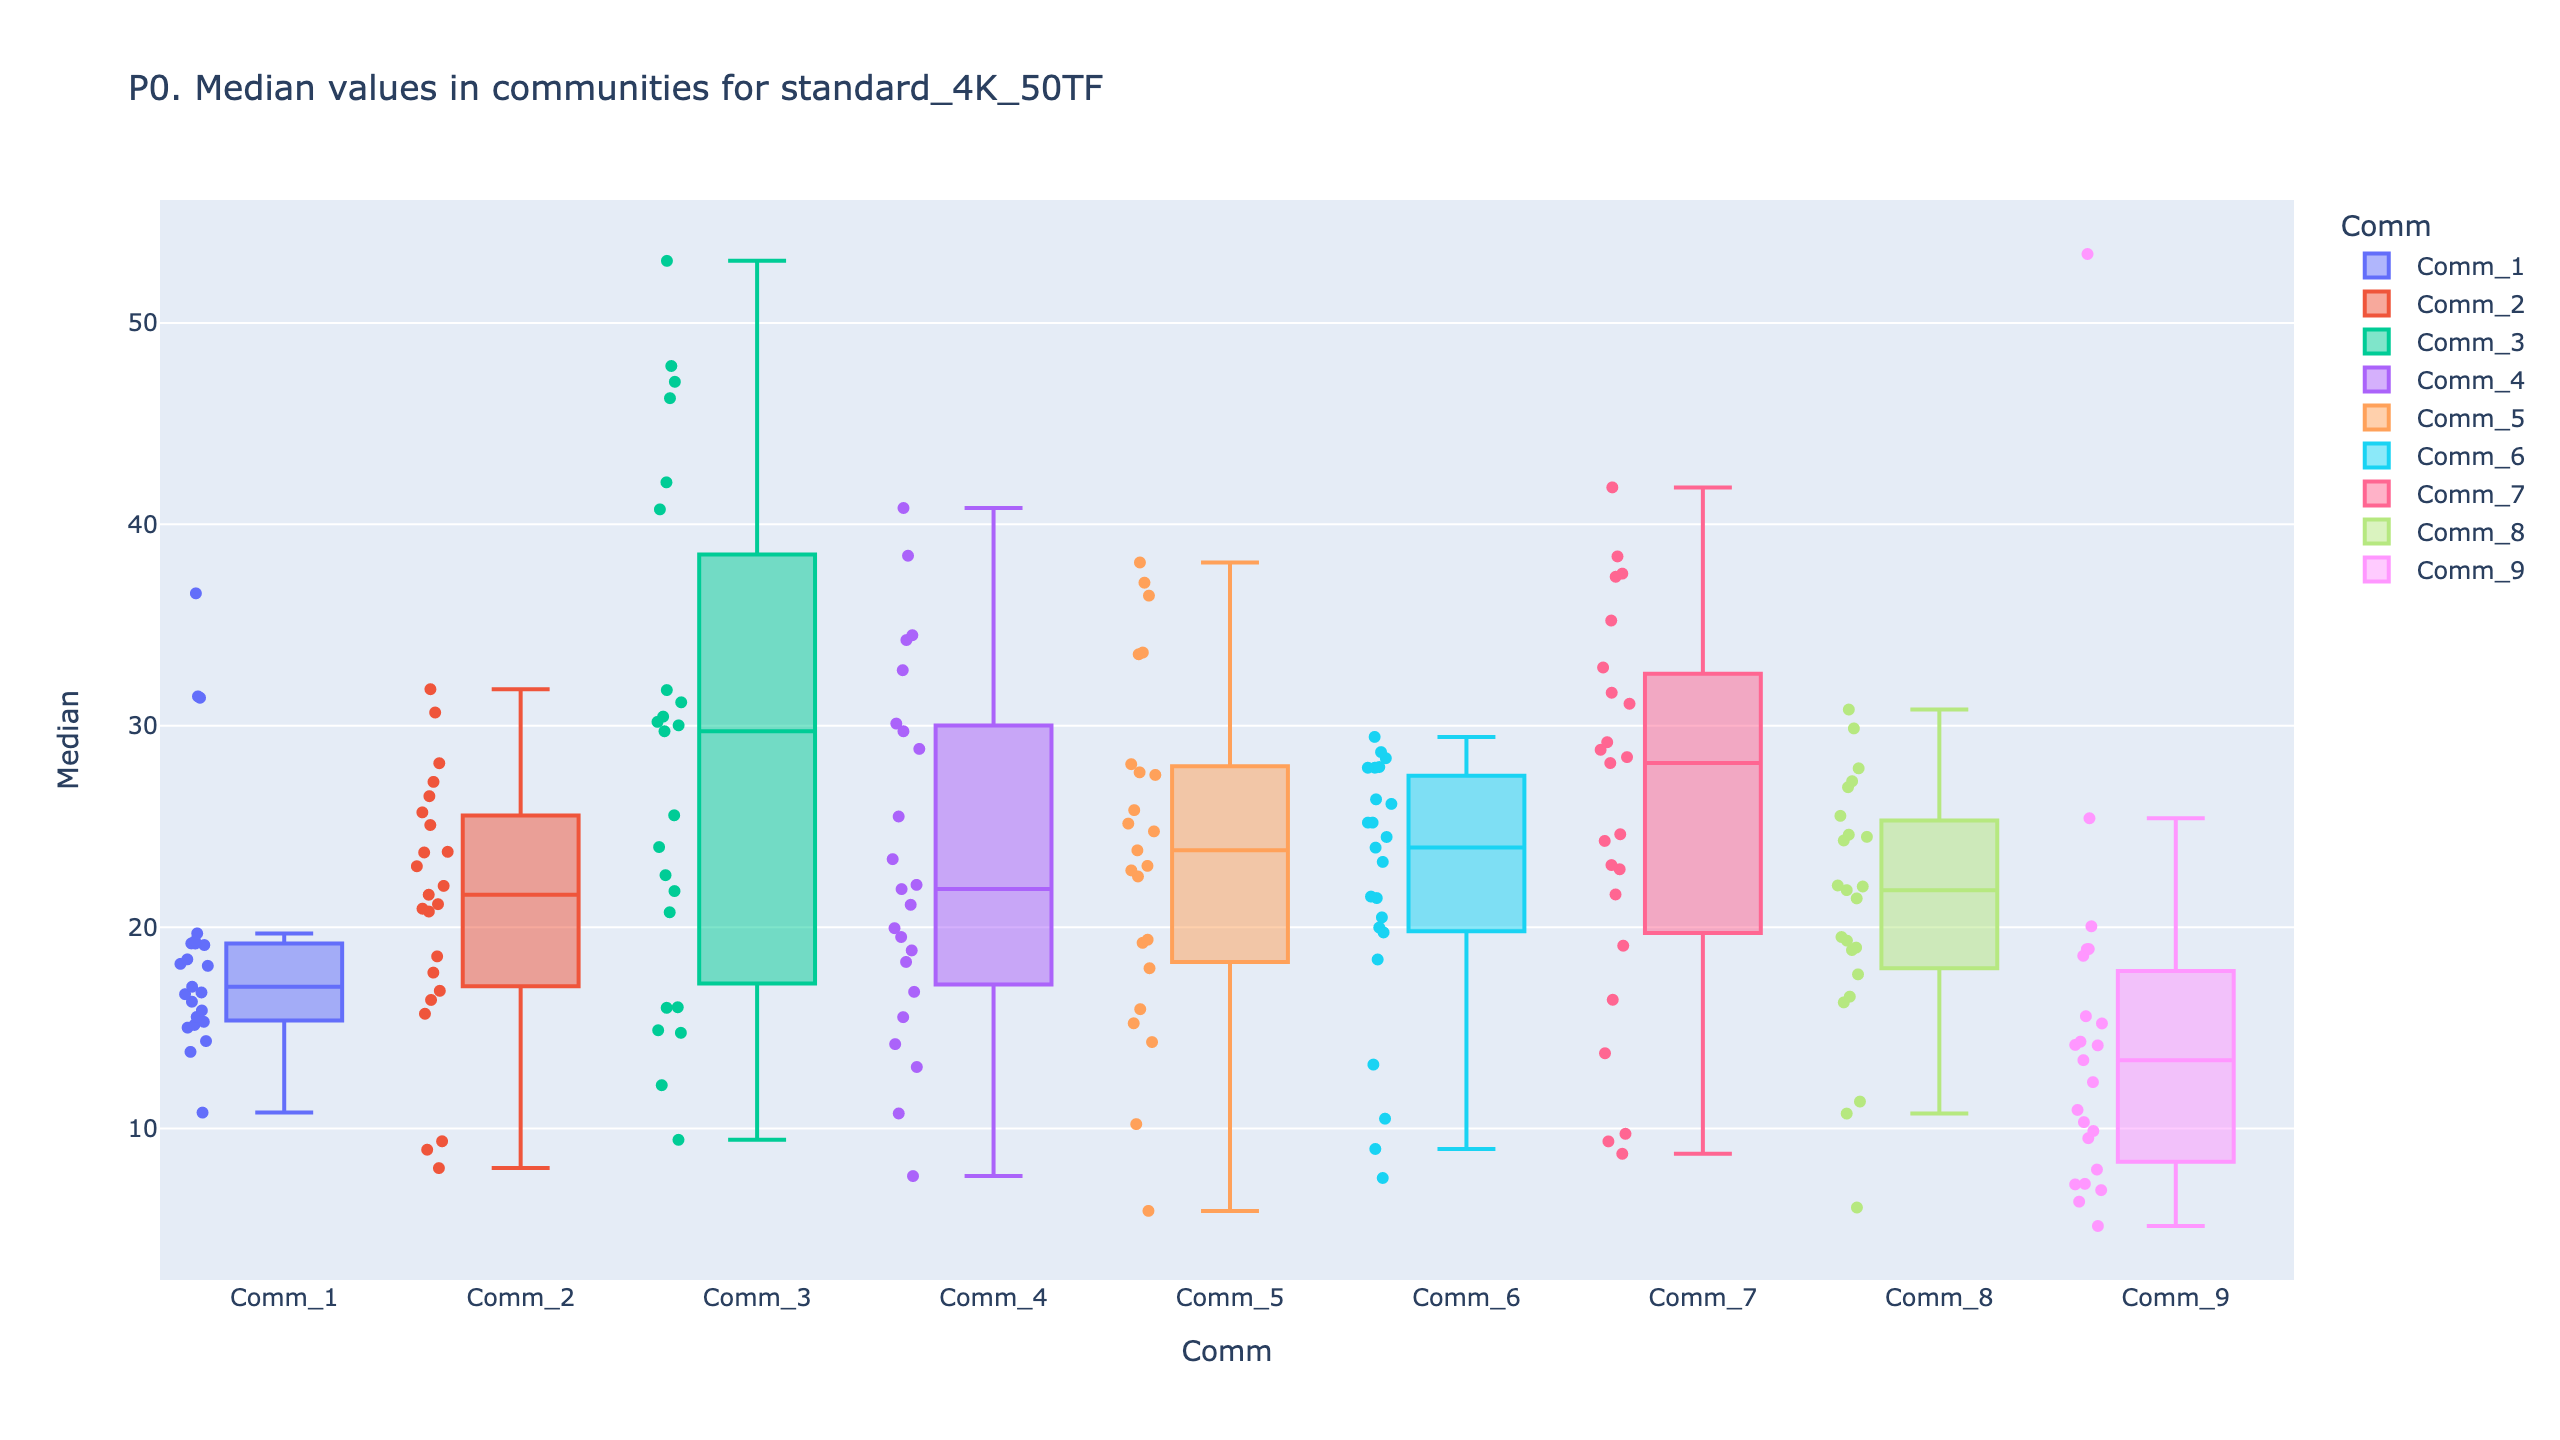
\includegraphics[width=\textwidth]{Images/P0/standard_4K_50TF_median.png}
        \caption{Standard median values}
    \end{subfigure}\hspace{\fill} % maximize horizontal separation
    \bigskip % more vertical separation
    \begin{subfigure}[t]{0.5\textwidth}
        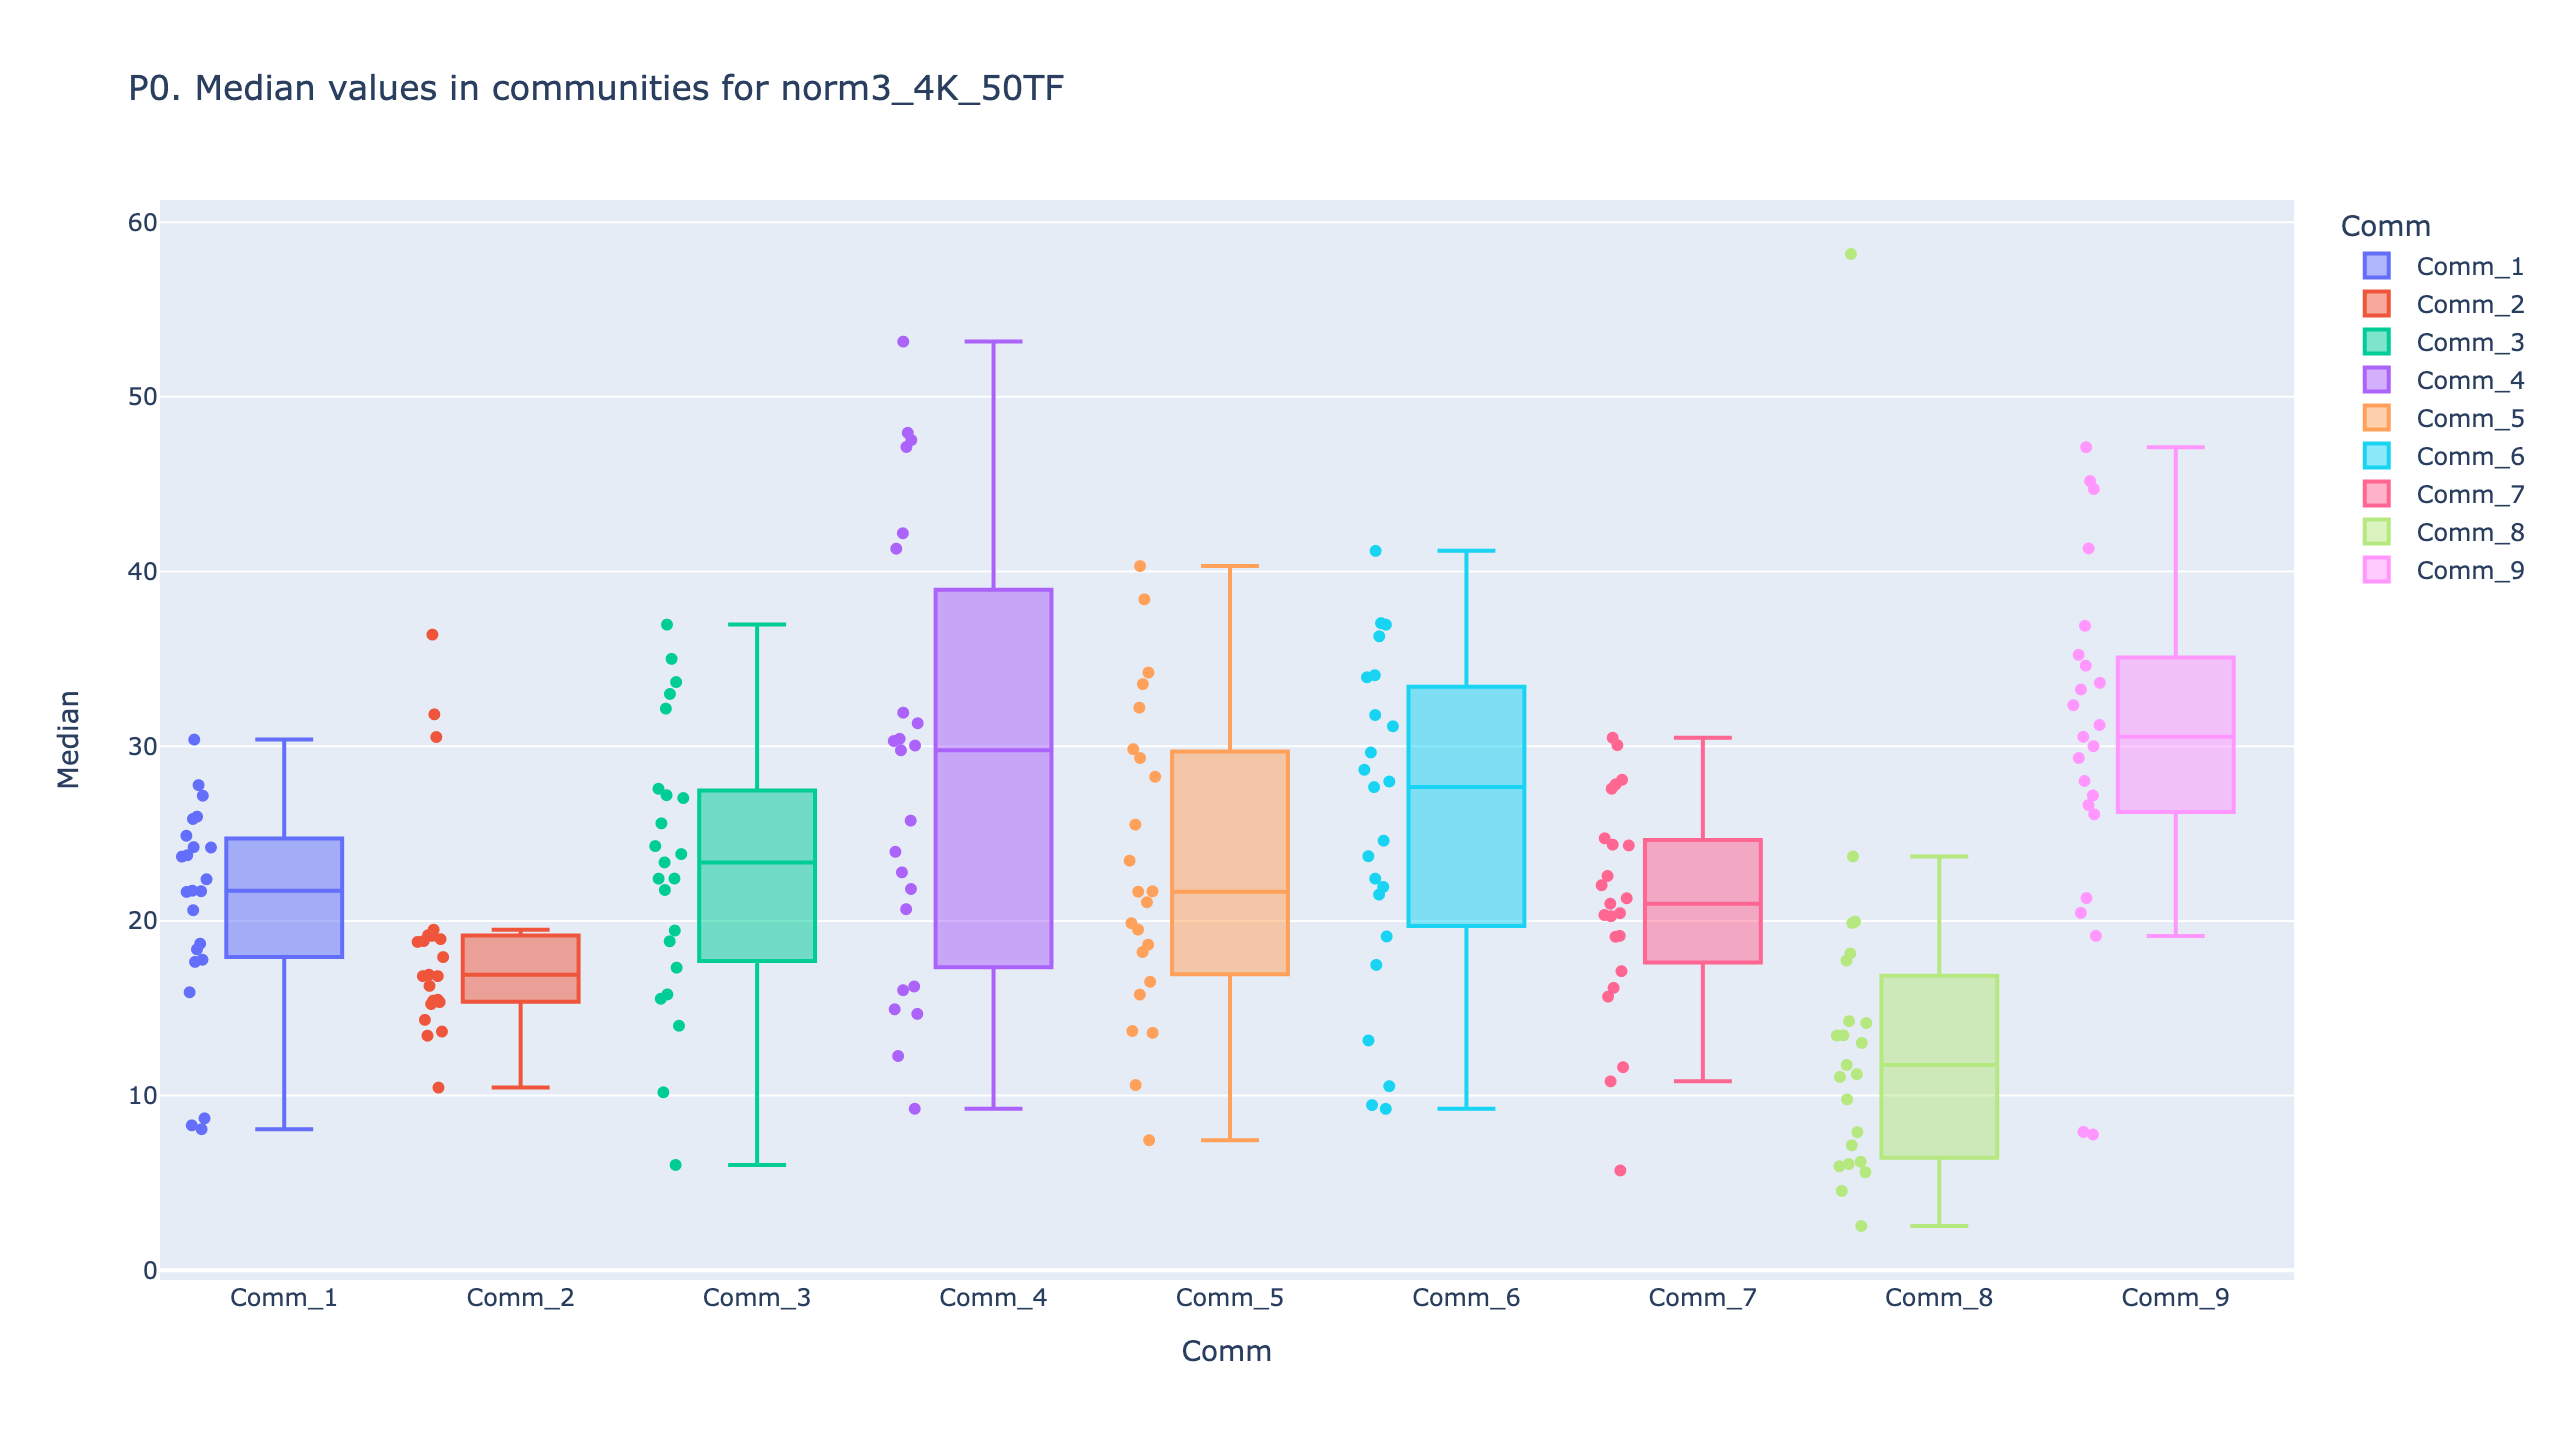
\includegraphics[width=\linewidth]{Images/P0/norm3_4K_50TF_median.png}
        \caption{Norm3 median values}
    \end{subfigure}\hspace{\fill} % maximize horizontal separation
    \caption{Median values for source and target}
    \label{fig:N_I:P0_median}
\end{figure}


\begin{figure}
    \captionsetup[subfigure]{justification=Centering}
    \begin{subfigure}[t]{0.5\textwidth}
        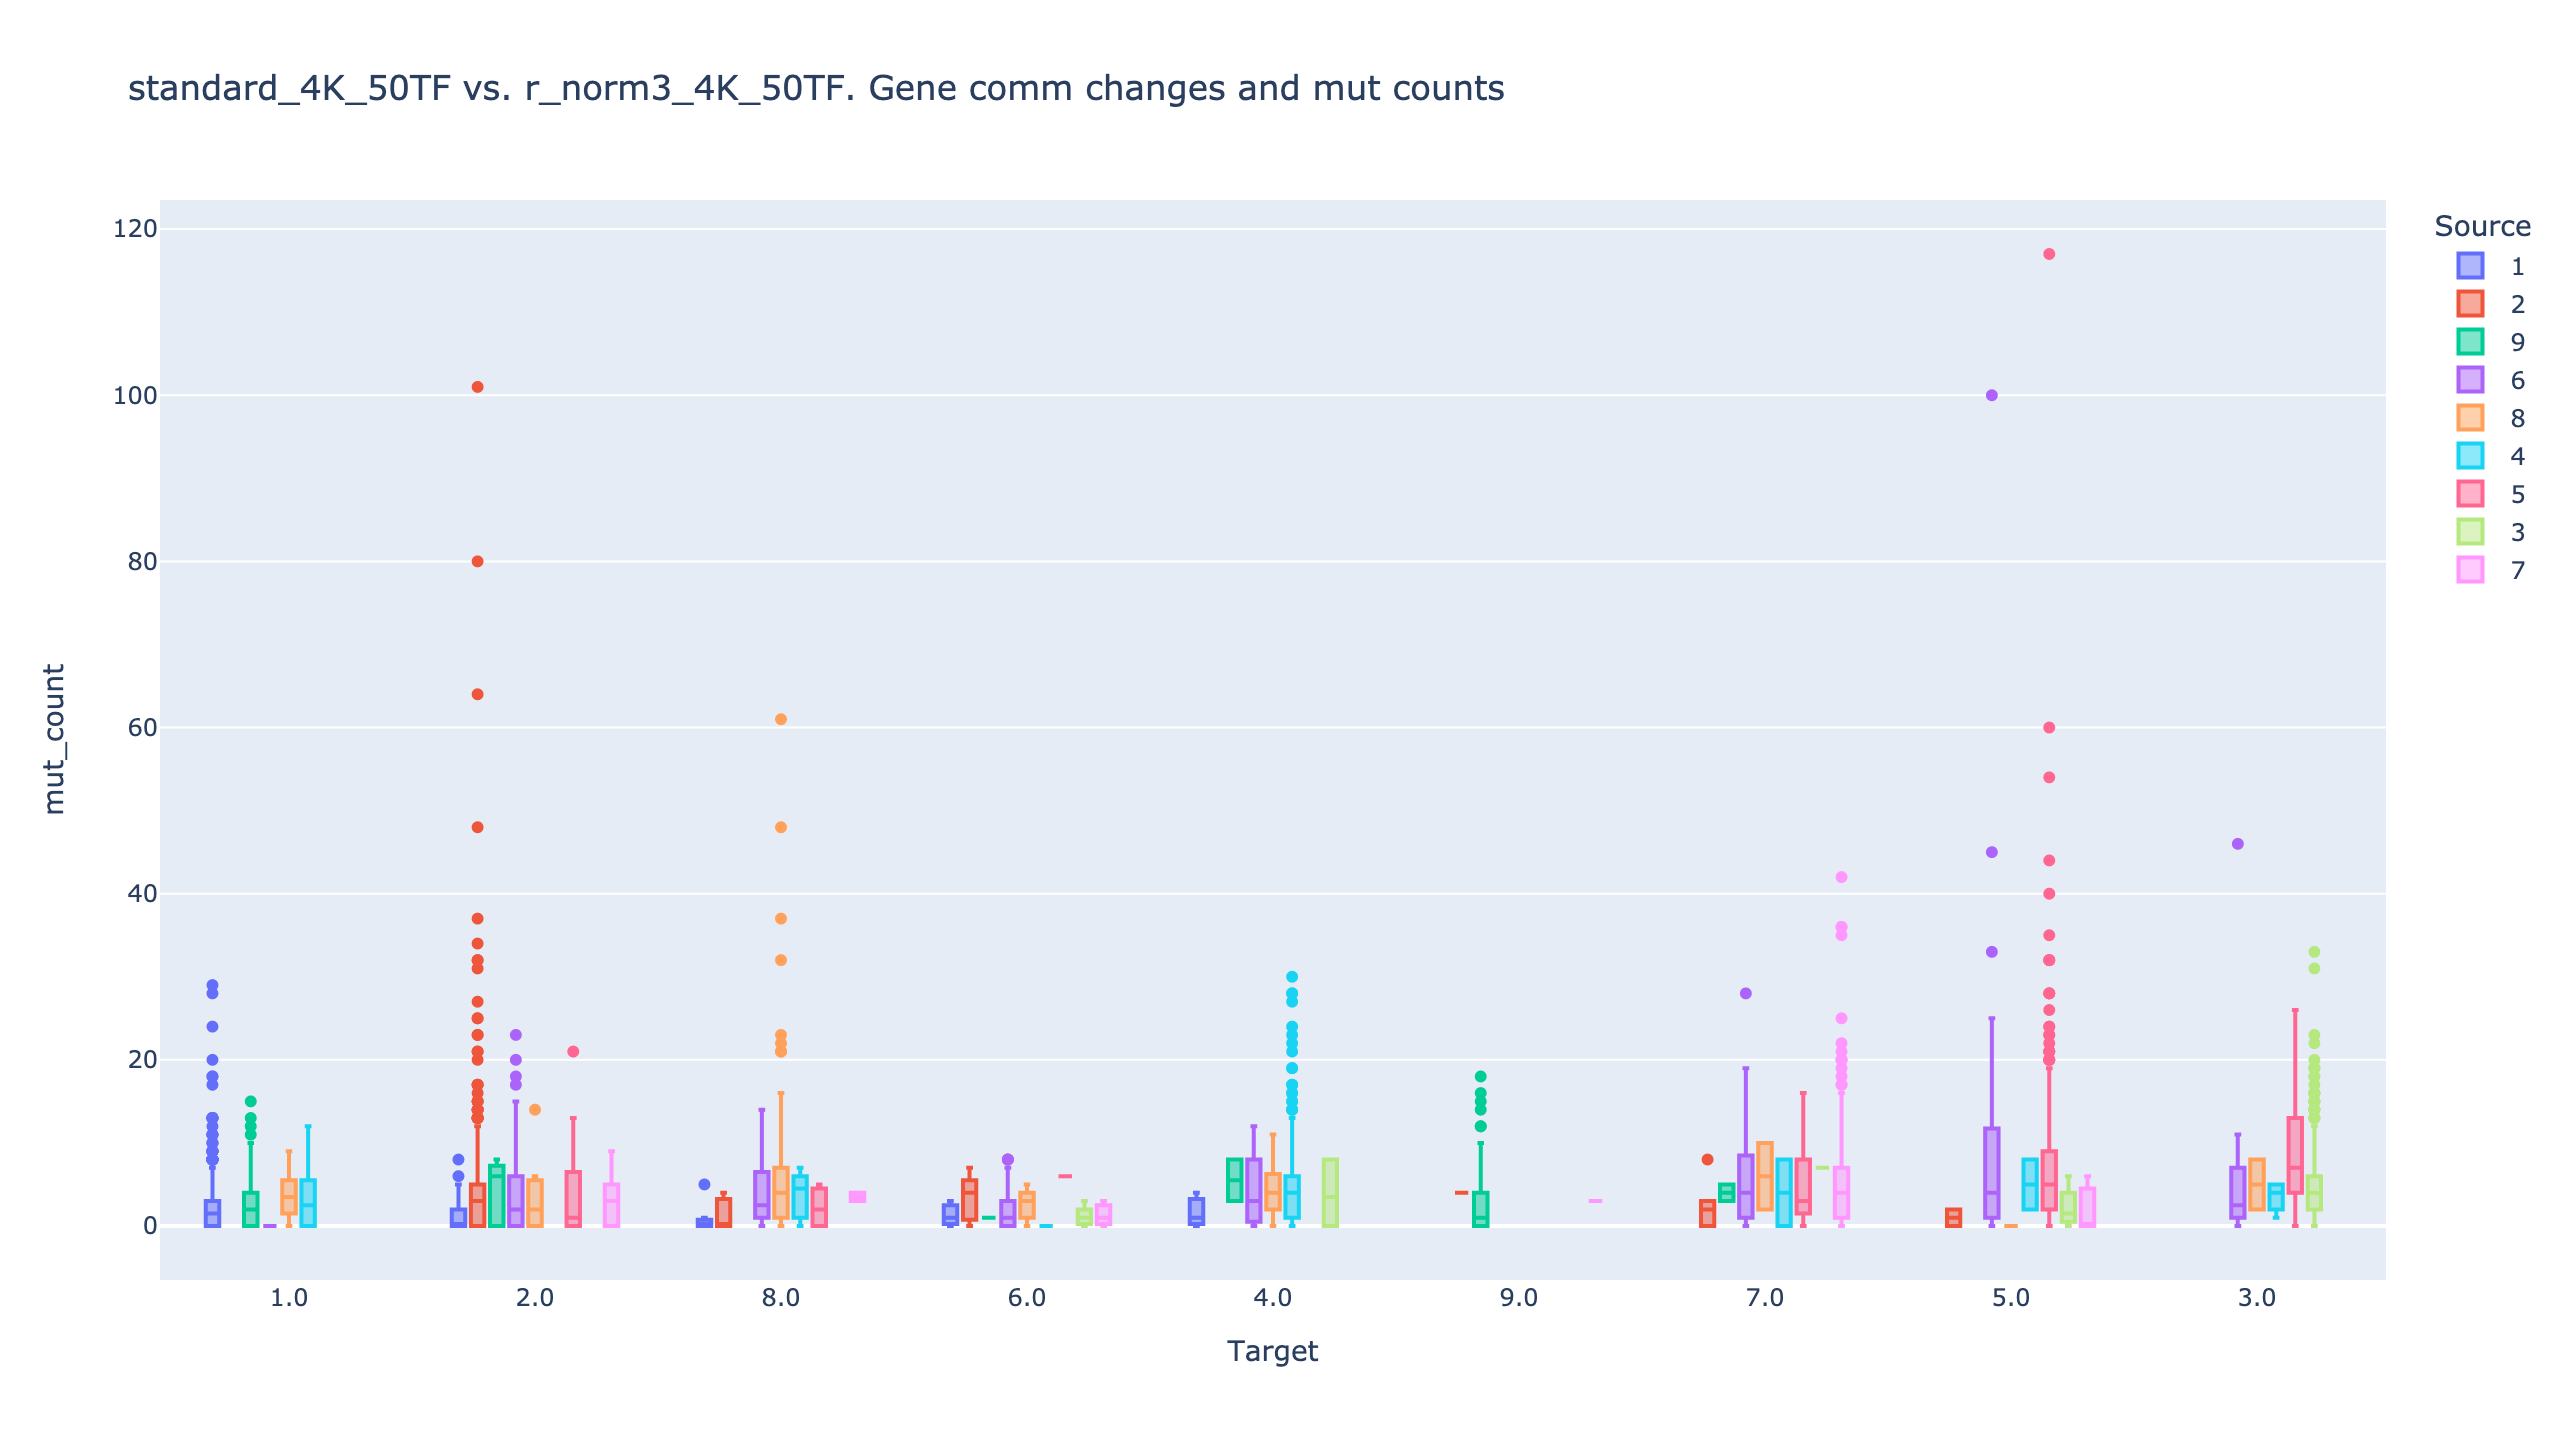
\includegraphics[width=\textwidth]{Images/P0/box_standard_4K_50TF_norm3_4K_50TF.png}
        \caption{Mutation count per community}
    \end{subfigure}\hspace{\fill} % maximize horizontal separation
    \begin{subfigure}[t]{0.5\textwidth}
        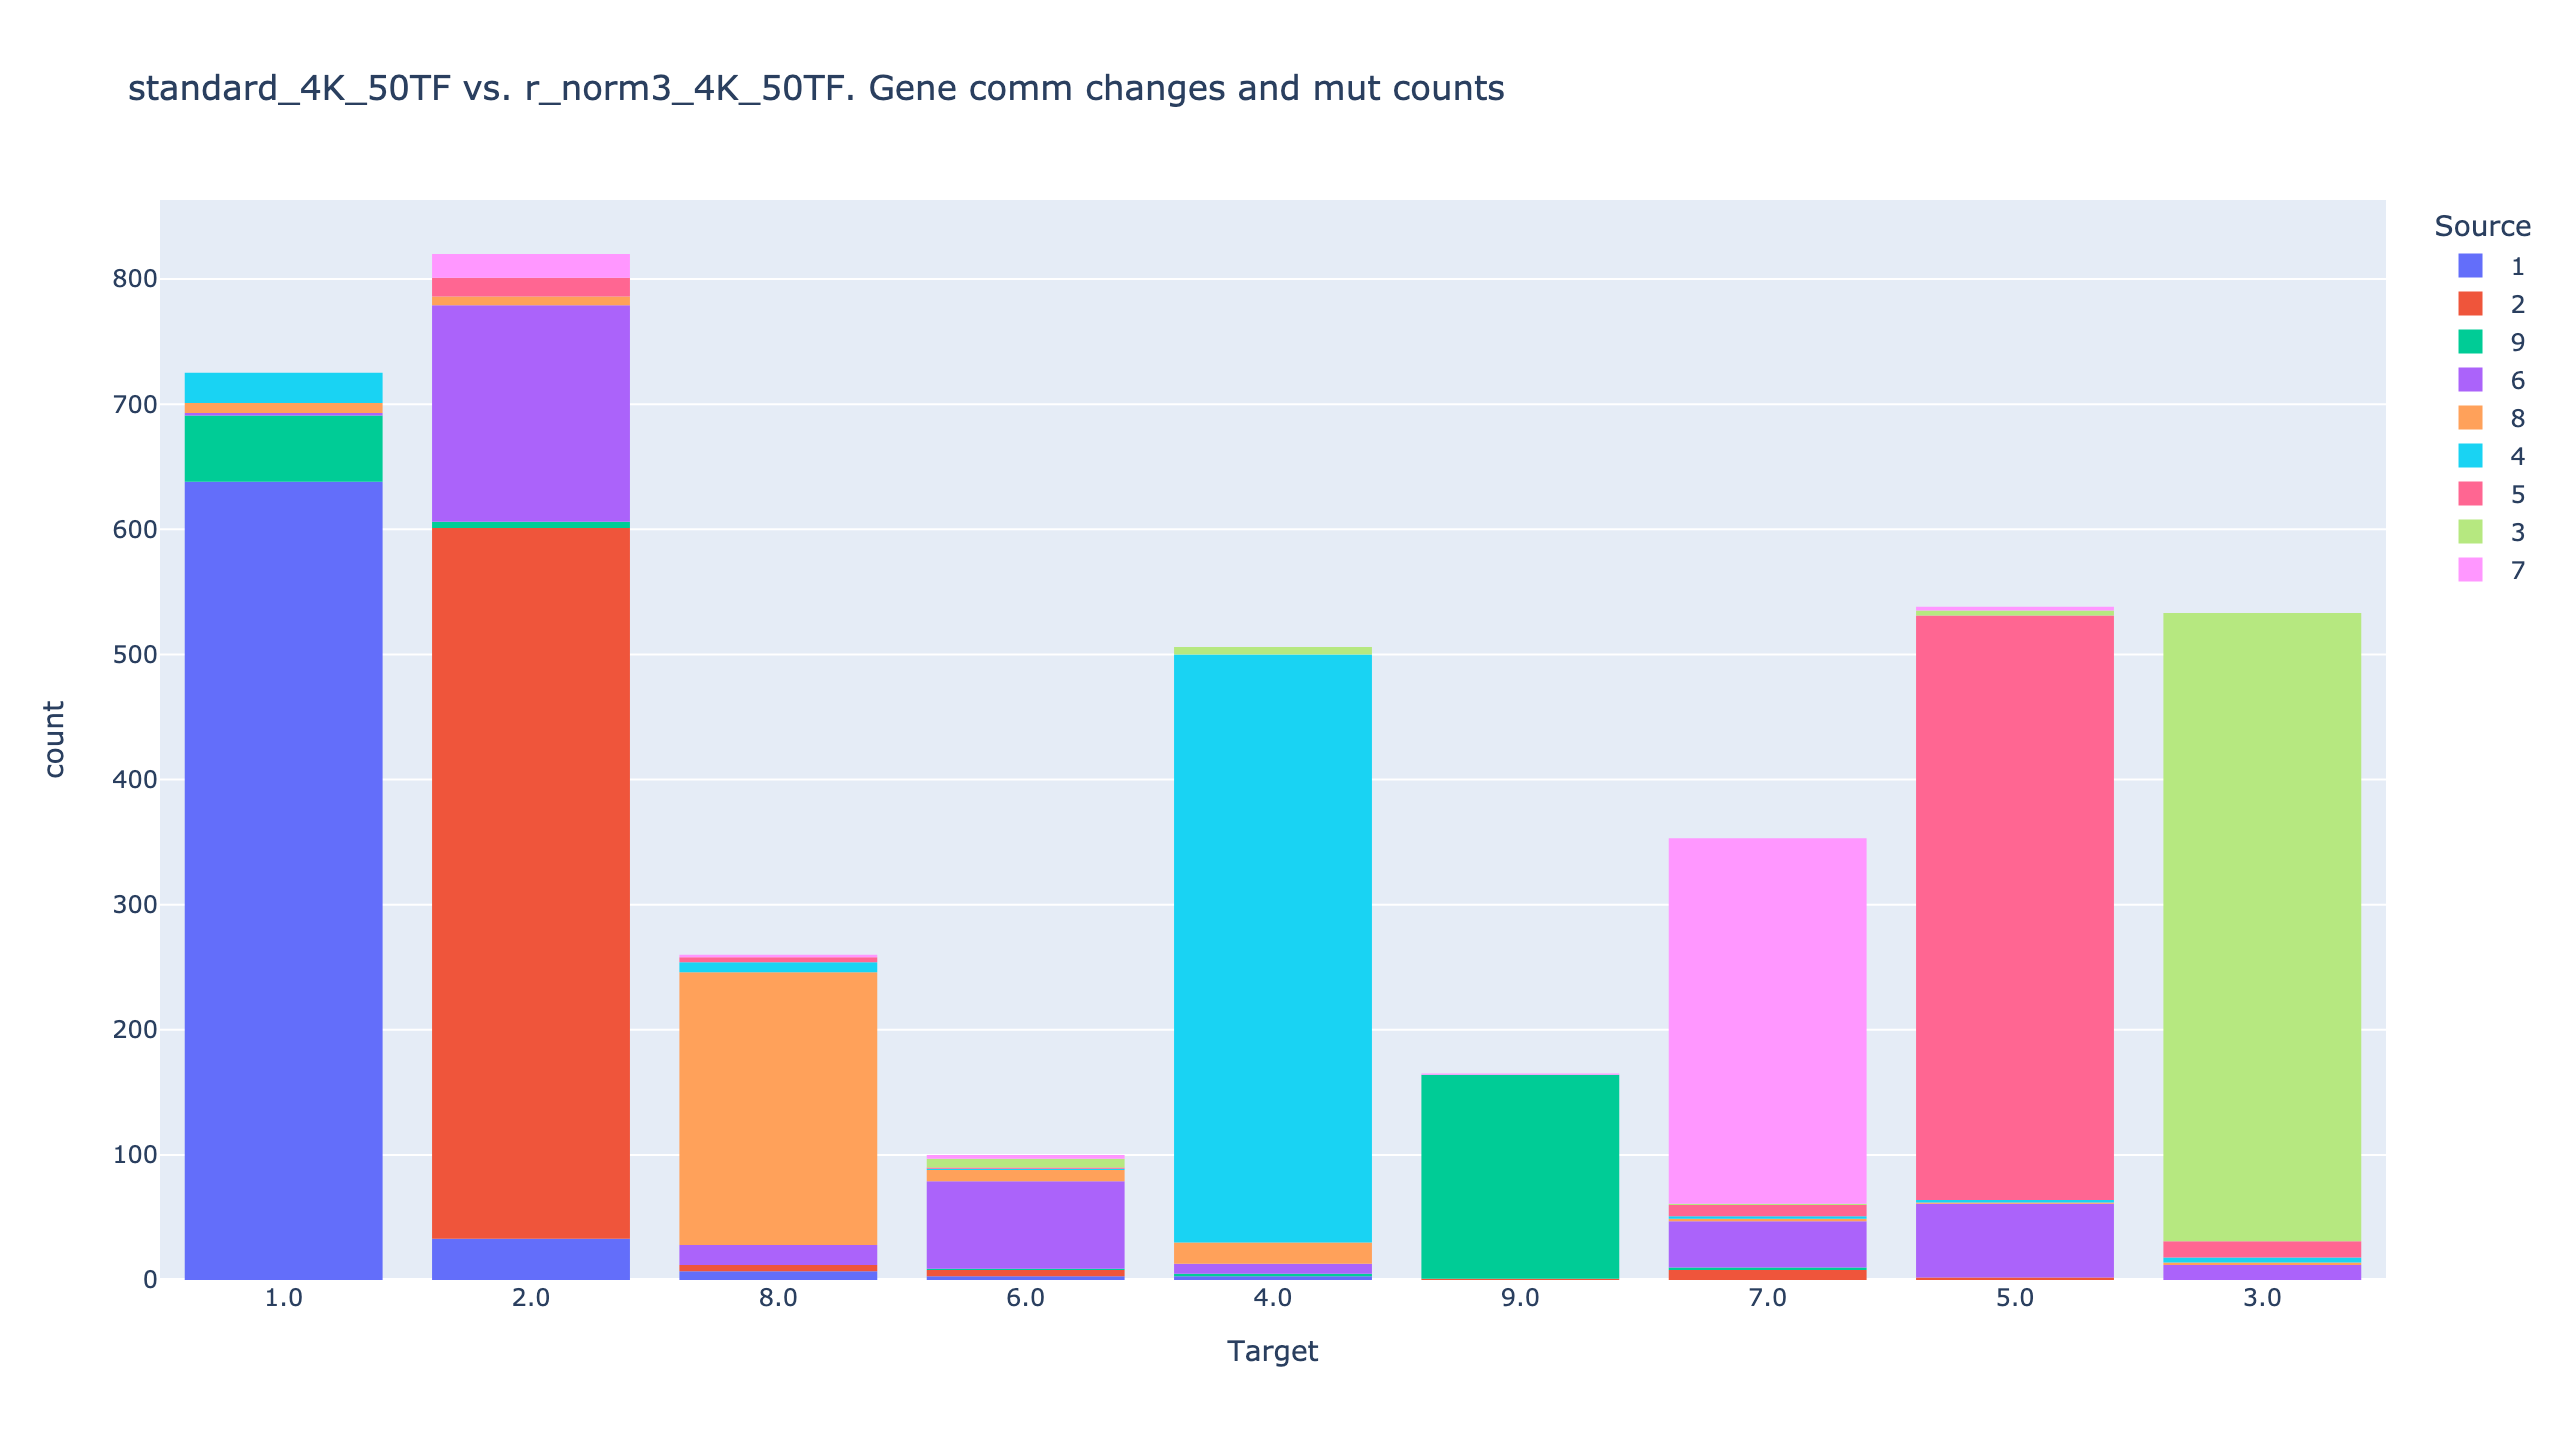
\includegraphics[width=\linewidth]{Images/P0/memberShip_standard_4K_50TF_norm3_4K_50TF.png}
        \caption{Membership changes}
    \end{subfigure}\hspace{\fill} % maximize horizontal separation
    \bigskip % more vertical separation
    \begin{subfigure}[t]{0.9\textwidth}
        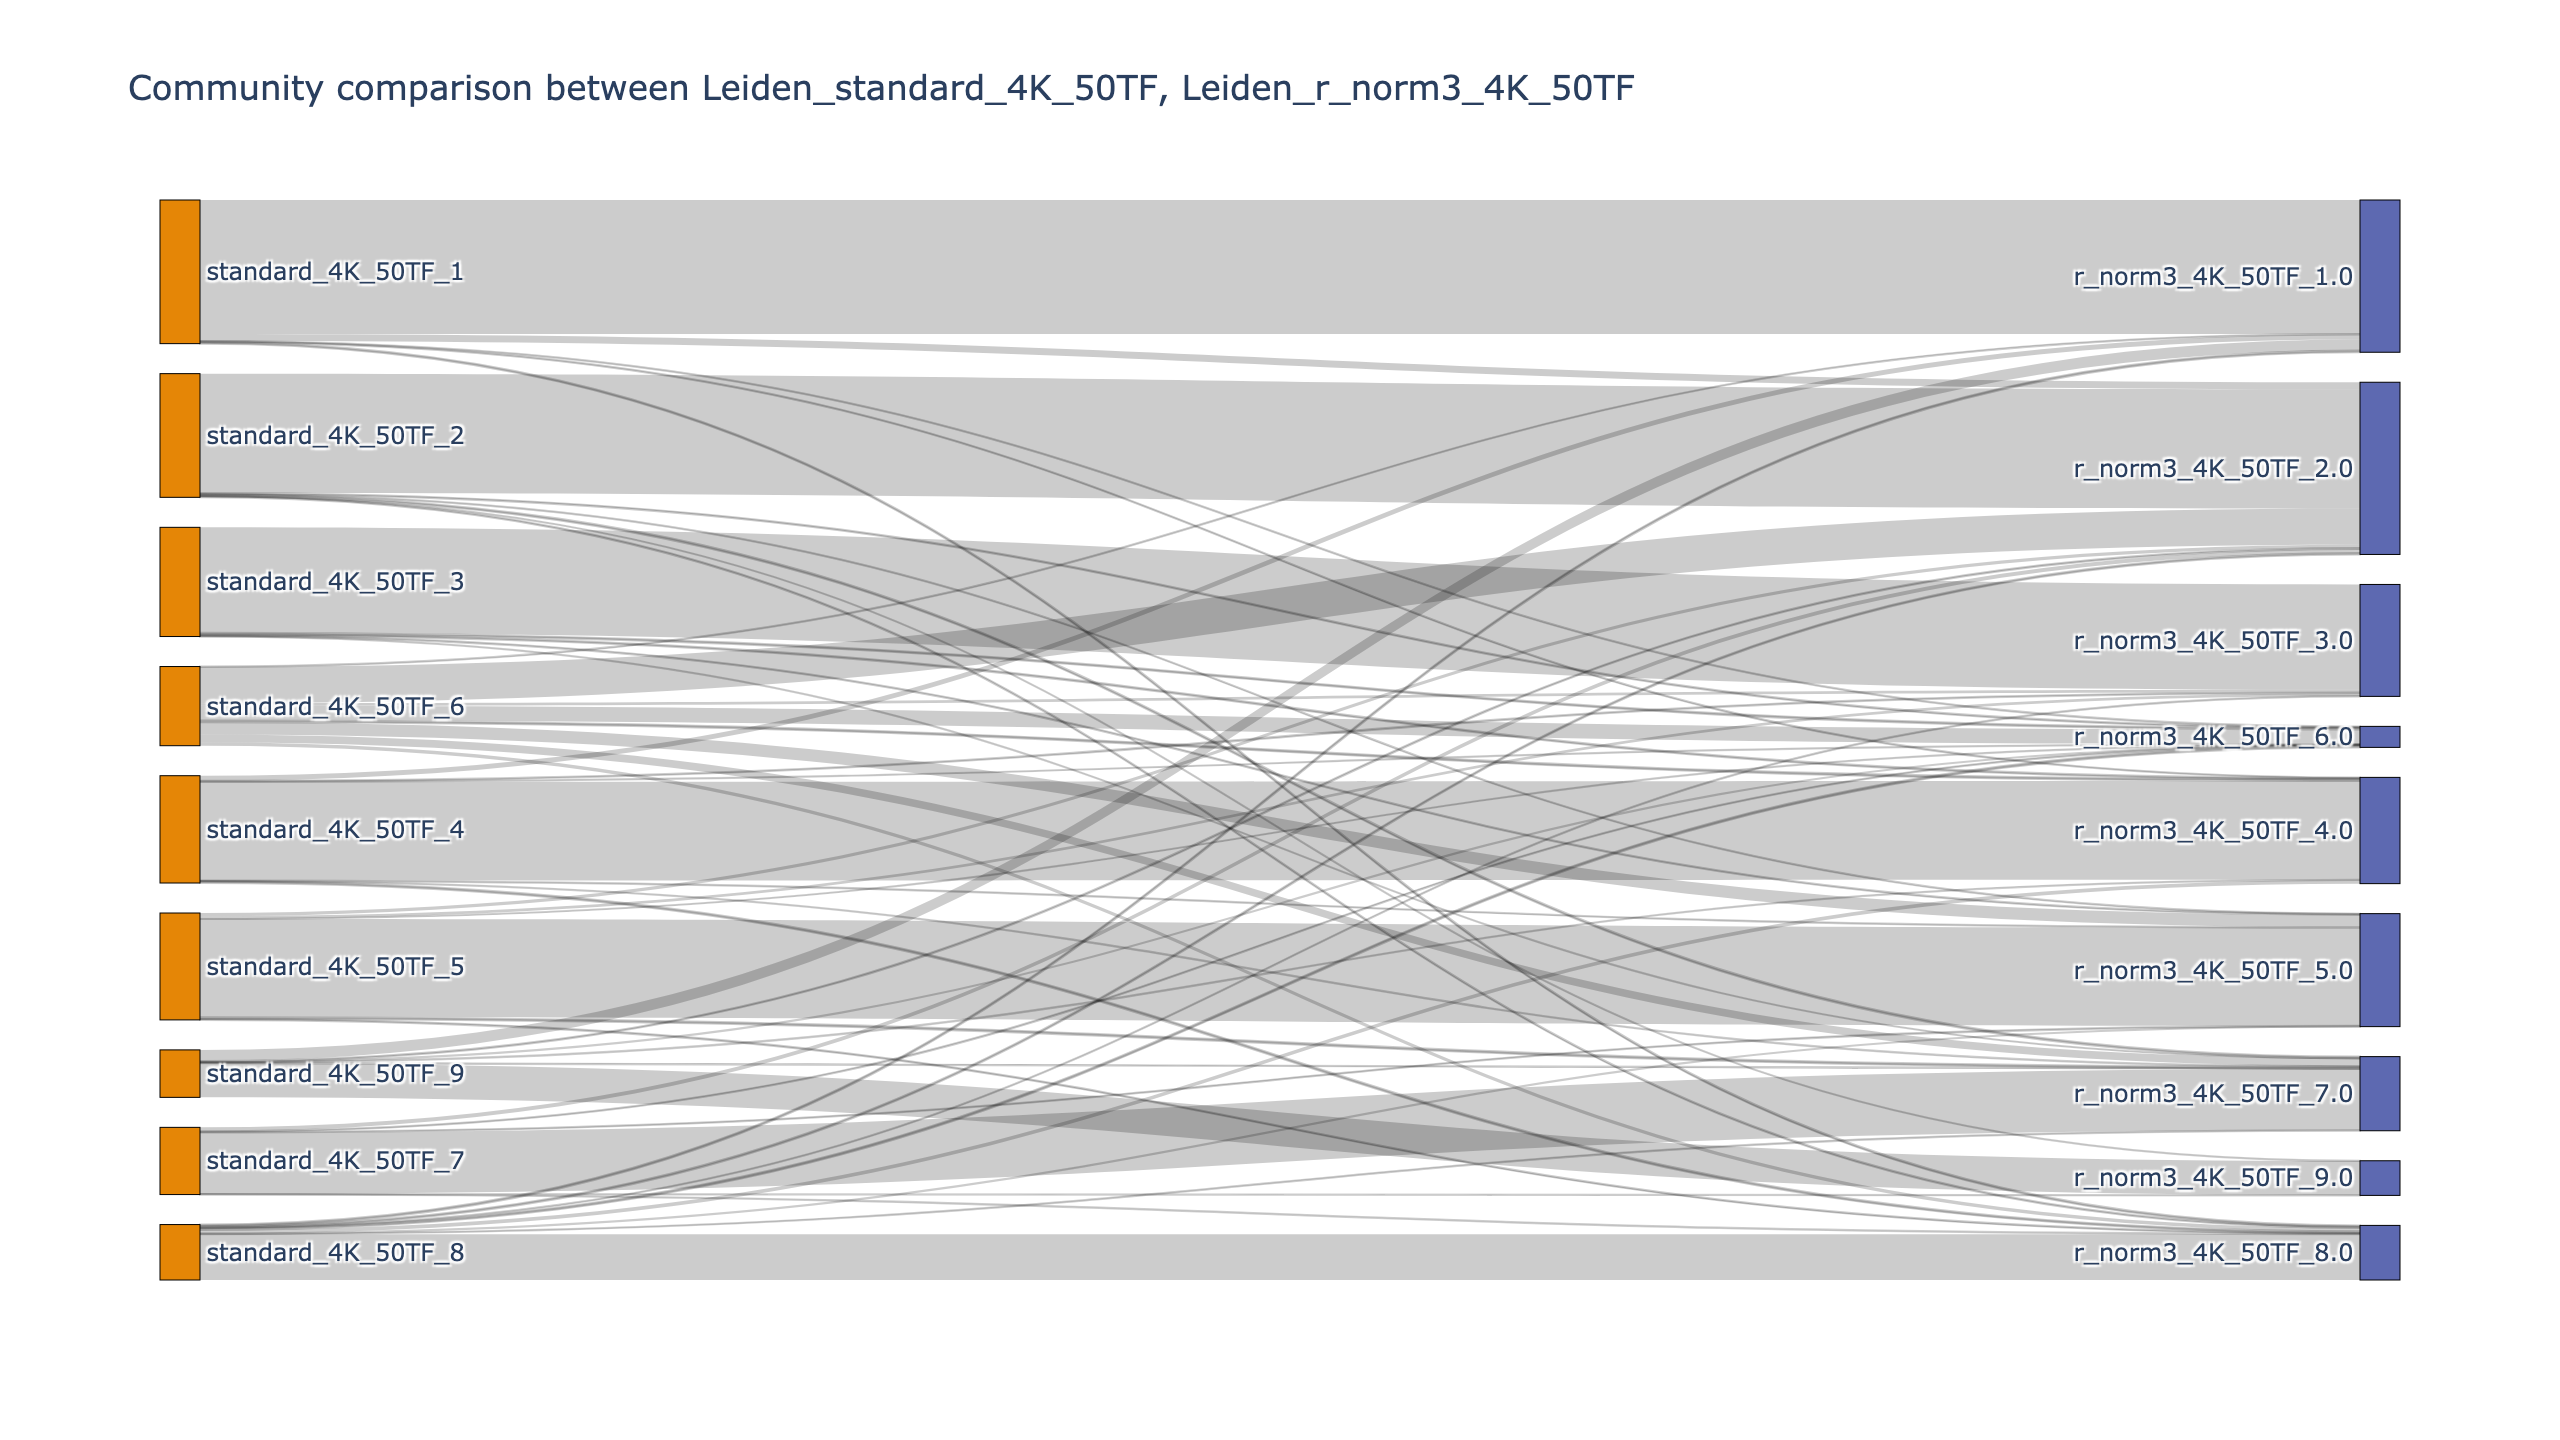
\includegraphics[width=\linewidth]{Images/P0/sankey_standard_4K_50TF_norm3_4K_50TF.png}
        \caption{Sankey between standard and norm3}
    \end{subfigure}\hspace{\fill} % maximize horizontal separation

    \caption{Comparison between Standard and norm3}
    \label{fig:N_I:P0_comp}
\end{figure}



\begin{figure}[!htb]
    \centering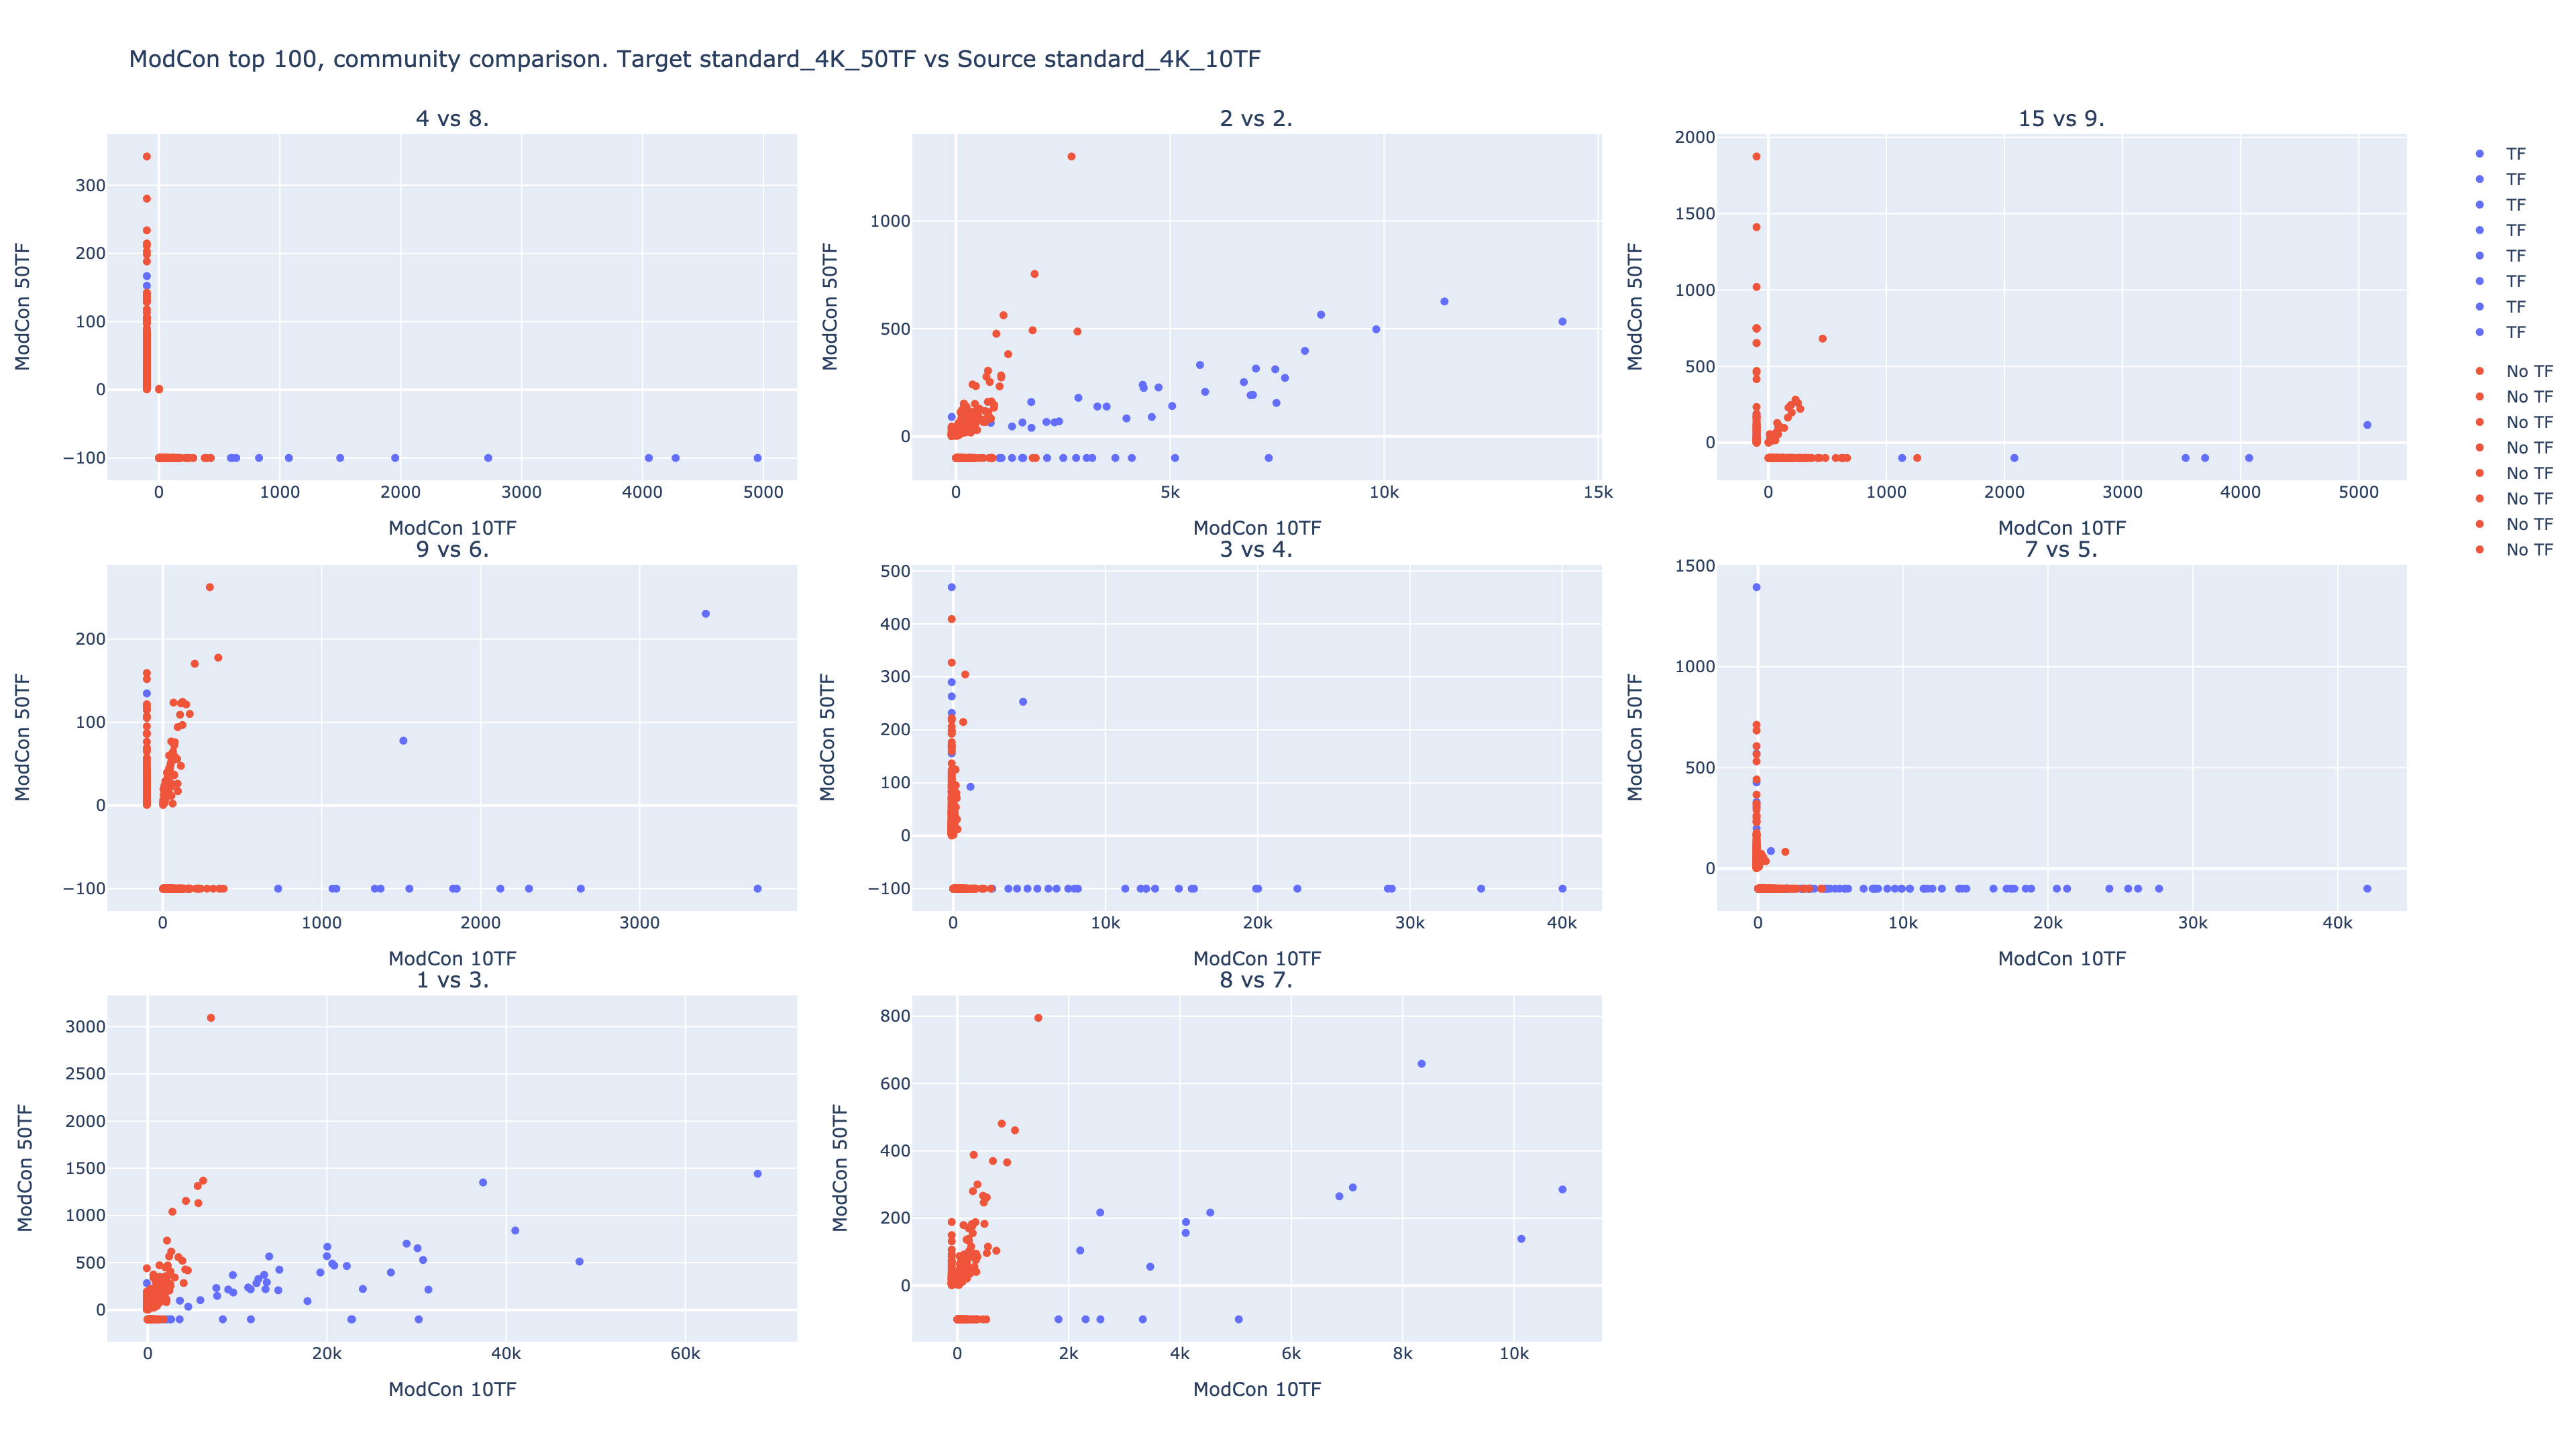
\includegraphics[width=1.0\textwidth,height=1.0\textheight,keepaspectratio]{Images/P0/TF_comp.png}
    \caption{TF Comparison}
    \label{fig:N_1:tf_comp}
\end{figure}

